% ========================================= TEMPLATE INFO ========================================
%
% Author:       P4ntomime
% Version:      1.0.0
% Last updated: 2024-02-18
% Brief:        A LaTeX template for summaries. See README.md for more information.
% 
% ================================================================================================
\documentclass[8pt, a4paper, twoside]{extarticle}
% Font size:    8pt
% Paper size:   A4
% style:        twoside (needed, so odd and even pages have different margins)
% orientation:  portrait. (use 'landscape' for landscape orientation)


% ========================================= DOCUMENT INFO =========================================
\def\title{Analog Microelectronics}                             % title
\def\shorttitle{AnME}                                           % short title (displayed as PDF title)
\def\dozent{Prof. Dr. Paul Zbinden}                             % lecturer
\def\semester{HS 2024}                                          % semester
\def\author{Flurin Brechbühler, Laurin Heitzer, Simone Stitz}   % authors
\def\repo{https://github.com/flurin-b/AnME}                     % repository link
\def\version{1.0.\today}                                        % version
\def\pagelimit{12}                                              % page limit -> causes pages after limit to be red
\def\titleoption{compact}                                       % options: compact, normal
\def\enableToC{true}                                            

% ================================= PACKAGES, SETUP AND COMMANDS ==================================
% =========================================== PACKAGES ============================================
\usepackage[utf8]{inputenc}         % input encoding: UTF-8
\usepackage[T1]{fontenc}            % font encoding: T1
\usepackage{textcomp}               % additional symbols
\usepackage{times}                  % times new roman font
\usepackage{inconsolata}            % use consolas font for ttfamily
\usepackage[main=ngerman]{babel}    % set main language to german


\usepackage{multicol}               % provides multicols environment
\usepackage{geometry}               % set page layout


\usepackage{enumitem}               % list customization
\usepackage[at]{easylist}               % easy lists
\usepackage{dirtree}                % tree style lists
\usepackage{outlines}               % easy nested lists
\usepackage{tabularx}               % some nicer tables with X columns
\usepackage{array}
\usepackage{makecell}               % multi-line cells in tables
\usepackage{multirow}               % multi-row cells in tables
\usepackage{hhline}                 % double lines in tables
\usepackage{booktabs}               % thick and thin lines in tables
\usepackage{boldline}               % bold (vertical) lines in tables
\usepackage{colortbl}               % colored tables


\usepackage{amsmath}                % math symbols
\usepackage{amssymb}                % more math symbols
\usepackage{mathtools}              % more math tools needed for pmatrix modification
\usepackage{mhsetup}                % needed to modify pmatrix environment
\usepackage{txfonts}                % Times math font
% \usepackage[squaren]{SIunits}       % SI-units
\usepackage{siunitx}                % qty for correct units
\sisetup{exponent-product = \cdot}  % set dot as product symbol
\usepackage{bm}                     % bold math symbols
\usepackage{trfsigns}               % needed for "Laplace" symbol (Korrespondenz)
\usepackage{mathrsfs}               % needed for Fourier transform "F"


\usepackage{graphicx}               % include graphics
\usepackage[inkscapelatex=false]{svg} % include svgs
\usepackage{graphbox}               % needed for aligning images in multicol environment
\usepackage{scalerel}               % scale any objects
\usepackage{anyfontsize}            % set any font size
\usepackage[table]{xcolor}          % needed for colors
\usepackage{pdfpages}               % include pdfs (with more options)


\usepackage{tcolorbox}              % colored boxes
\usepackage[outline]{contour}       % contour for text (used in custom underline command)
\usepackage[normalem]{ulem}         % custom underline (used in custom underline command)


\usepackage{tikz}                   % needed for TikZ drawings


\usepackage{listings}               % for nicer code display
% to use nodes inside listing see: https://texample.net/tikz/examples/tikz-listings/


\usepackage{hyperref}               % clickable links
\usepackage{qrcode}                 % QR code generation (also clickable)


\usepackage{ifthen}                 % if-then-else commands
\usepackage{calc}                   % simple arithmetic in LaTeX commands


\usepackage{draftwatermark}         % watermark on pages after a certain limit
\usepackage{fancyhdr}               % custom header and footer
\usepackage[explicit]{titlesec}     % custom section titles


\usepackage{datetime2}              % custom date format for versioning


% ========================================== BASIC SETUP ==========================================

% --------------------------------------- DOCUMENT SETTINGS ---------------------------------------
\hypersetup{hidelinks,
% set pdf metadata
            pdfauthor={\author},
            pdftitle={\shorttitle},
            pdfsubject={\title\ \semester},
            pdfkeywords={Gahn go lerne!!}}

% set style for URLs
\urlstyle{same} % sets url font to the same as the preceeding text

% set page layout
\geometry{left=3mm, 
          right=3mm, 
          top=3mm, 
          bottom=6mm, 
          headheight=0mm, 
          headsep=0mm, 
          footskip=4mm}

\setlength{\columnsep}{1.5mm}       % distance between columns
\setlength{\columnseprule}{0.1pt}   % thickness of column separation line
\setlength{\parindent}{0pt}         % no paragraph indentation

\setcounter{tocdepth}{2}            % only display sections and subsections in toc
% \setcounter{secnumdepth}{0}       % uncomment to disable section numbering

\DeclareMathSizes{8}{8}{6}{5}       % set math font sizes for 8pt document


% --------------------------------------- COLOR DEFINITIONS ---------------------------------------
\definecolor{sectioncolor}{HTML}{ffc81a}
\definecolor{subsectioncolor}{HTML}{ffe697}
\definecolor{sectextcol}{HTML}{000000}
\definecolor{subsectextcol}{HTML}{000000}

\definecolor{backcolour}{HTML}{f5f5f0} % background color for highlighted text

% TODO: define color palette
% color palette: https://colorkit.co/color-palette-generator/FF8552-9e22bd-404E7C-C32E15-225A28/
\definecolor{green}{HTML}{1af430}
\definecolor{red}{HTML}{f90d09}
\definecolor{blue}{HTML}{093ce5}
\definecolor{orange}{HTML}{f7730e}
\definecolor{violet}{HTML}{a516c9}

% colors for listings (code)
\definecolor{commentcolour}{HTML}{6a9955}
\definecolor{keywordcolour}{HTML}{7f0055}
\definecolor{stringcolour}{HTML}{9e22bd}
\definecolor{numbercolour}{HTML}{808080}


% ----------------------------------- LIST AND TABULAR SETTINGS -----------------------------------
\setlist[enumerate]{%
    labelindent=0pt,                                % no indentation for labels
    labelwidth = \widthof{\ref{enum-\EnumitemId}},  % set label width to widest label
    label=\bfseries\arabic*.,                       % label style bold arabic numerals (1., 2., ...)
    itemindent=1ex,                                 % separation between label and item text
    leftmargin=!,                                   % automatically calculate left margin
    after=\label{enum-\EnumitemId}}                 % set label for referencing in labelwidth

\setlist[itemize]{leftmargin=1.5em}                 % left margin for itemize: 1.5em
\setlist[description]{leftmargin=2ex}               % left margin for description: 2ex
\setlist{nosep}                                     % no vertical spacing between list items

\renewcommand{\arraystretch}{1}                     % stretch table rows

\setcounter{MaxMatrixCols}{32}                      % increase max columns in matrix environments

% ----------------------------------------- TIKZ SETTINGS -----------------------------------------
\usetikzlibrary{arrows}
\usetikzlibrary{arrows.meta}
\usetikzlibrary{bending}
\usetikzlibrary{decorations.pathreplacing}
\usetikzlibrary{decorations.markings}
\usetikzlibrary{angles}
\usetikzlibrary{tikzmark}
\usetikzlibrary{petri}
\usetikzlibrary{positioning}
\usetikzlibrary{shapes}
\usetikzlibrary{shapes.arrows}
\usetikzlibrary{calc}
\usetikzlibrary{fit}


% ------------------------------------ OTHER PACKAGE SETTINGS -------------------------------------

% define and set new date style for versioning as YYYYMMDD
\DTMnewdatestyle{vnumdate}{%
    \renewcommand{\DTMdisplaydate}[4]{\number##1\DTMtwodigits{##2}\DTMtwodigits{##3}}%
    \renewcommand{\DTMDisplaydate}{\DTMdisplaydate}%
}
\DTMsetdatestyle{vnumdate}


% setup for ulem and contour packages
\renewcommand{\ULdepth}{1.75pt} % set underline depth
\contourlength{0.7pt}           % set contour length

% use xparse library in tcolorbox (for \DeclareTotalTCBox etc.)
\tcbuselibrary{xparse}

% ====================================== SETUP AND COMMANDS =======================================

% custom font size for paragraph
\newcommand{\semilarge}{\fontsize{9}{8}\selectfont}

\ExplSyntaxOn
% custom underline command for exclusions on lowercase letters such as g, j, p, q, y
\newrobustcmd{\myul}[1]{%
    \if_mode_math:
        \text{%
            \uline{\phantom{$#1$}}%
            \llap{\contour{white}{$#1$}}%
        }
    \else:
        \uline{\phantom{#1}}%
        \llap{\contour{white}{#1}}%
    \fi:
}

\renewrobustcmd{\underline}[1]{%
    \if_mode_math:
        \text{%
            \uline{\phantom{$#1$}}%
            \llap{\contour{white}{$#1$}}%
        }
    \else:
        \uline{\phantom{#1}}%
        \llap{\contour{white}{#1}}%
    \fi:
}
\ExplSyntaxOff

% custom command for straight double quotes
\newcommand{\qts}[1]{\textquotedbl#1\textquotedbl}

% setup header and footer
\pagestyle{fancy}
\fancyhf{}                          % clear all header and footer fields
\renewcommand{\headrulewidth}{0pt}  % remove header rule
\renewcommand{\footrulewidth}{0pt}  % remove footer rule
\fancyfoot[C]{\thepage}             % page number in center of footer


% --------------------------------------- TITLE FORMATTING ----------------------------------------

\titleclass{\part}{straight}
% part formatting
\titleformat{\part}
            {\huge\bfseries}
            {\thepart}
            {1em}
            {#1}

\titleformat{\section}
            % {\fontsize{9}{8}\selectfont\bfseries}
            {\Large\bfseries}
            {}
            {0mm}
            {\tikz{
                \node[fill=sectioncolor,            % fill color:       sectioncolor
                      text=sectextcol,              % text color:       sectextcol
                      text width=\columnwidth-4pt,  % text width:       columnwidth - 2x padding
                      text depth=0pt,               % text depth:       0pt (needed so text stays vertically centered)
                      minimum height=5mm,           % minimum height:   5mm
                      inner sep=2pt,                % inner padding:    2pt
                      align=left]                   % text alignment:   left
                      {\thesection\ #1};}}

\titleformat{numberless, name=\section}
            % {\fontsize{9}{8}\selectfont\bfseries}
            {\Large\bfseries}
            {}
            {0mm}
            {\tikz{
                \node[fill=sectioncolor,            % fill color:       sectioncolor
                      text=sectextcol,              % text color:       sectextcol
                      text width=\columnwidth-4pt,  % text width:       columnwidth - 2x padding
                      text depth=0pt,               % text depth:       0pt (needed so text stays vertically centered)
                      minimum height=5mm,           % minimum height:   5mm
                      inner sep=2pt,                % inner padding:    2pt
                      align=left]                   % text alignment:   left
                      {#1};}}

\titlespacing{\section}
             {0mm}
             {.2ex}
             {.2ex}


% subsection formatting
\titleformat{\subsection}
            {\large\bfseries}
            {}
            {0mm}
            {\phantomsection\tikz{
                \node[fill=subsectioncolor,         % fill color:       subsectioncolor 
                      text=subsectextcol,           % text color:       subsectextcol 
                      text width=\columnwidth-4pt,  % text width:       columnwidth - 2x padding 
                      text depth=0pt,               % text depth:       0pt (needed so text stays vertically centered)
                      minimum height=5mm,           % minimum height:   5mm 
                      inner sep=2pt,                % inner padding:    2pt 
                      align=left]                   % text alignment:   left
                      {\thesubsection\ #1};}}

\titleformat{numberless, name=\subsection}
            {\large\bfseries}
            {}
            {0mm}
            {\phantomsection\tikz{
                \node[fill=subsectioncolor,         % fill color:       subsectioncolor 
                      text=subsectextcol,           % text color:       subsectextcol 
                      text width=\columnwidth-4pt,  % text width:       columnwidth - 2x padding 
                      minimum height=5mm,           % minimum height:   5mm 
                      inner sep=2pt,                % inner padding:    2pt 
                      align=left]                   % text alignment:   left
                      {#1};}}

\titlespacing{\subsection}
             {0mm}
             {1ex}
             {.2ex}


% subsubsection formatting
\titleformat{\subsubsection}
            {\large\bfseries}
            {\myul{\thesubsubsection\ }}
            {0mm}
            {\phantomsection{}\myul{#1}}

\titlespacing{\subsubsection}
             {0mm}
             {1ex}
             {1ex}


% paragraph formatting
\titleformat{\paragraph}
            {\semilarge\bfseries}
            {}
            {0mm}
            {#1\normalfont :\;}

\titlespacing{\paragraph}
             {0mm}
             {1.5ex}
             {0.1ex}


% new alias for paragraph '\para' (shorter than \paragraph)
\let\para\paragraph%

% custom command for examples
\newcommand{\example}[1]{\subsubsection*{Example: #1}}


% ----------------------------------- CUSTOM TABULAR SPECIFIERS -----------------------------------

% centered fixed width column type
\newcolumntype{P}[1]{>{\centering\arraybackslash}p{#1}}

 % centered variable width column type
\newcolumntype{C}{>{\centering\arraybackslash}X}

% centered math column type
\newcolumntype{M}{>{$}c<{$}}

% centered colored column type
\newcolumntype{Q}[3]{>{\footnotesize\color{#1}\columncolor{#2}\centering\arraybackslash}m{#3}}

% custom big strut for vertical spacing in tables
\newcommand{\bigstrut}{\rule[-.3\baselineskip]{0pt}{1.1\baselineskip}}

% inline tikz node for later referencing
\newcommand{\tikznode}[2]{% from https://tex.stackexchange.com/a/402466/121799
	\ifmmode%
	\tikz[remember picture,baseline= (#1.base)] \node[inner sep=0pt, draw=none, minimum width=0mm, minimum height=0mm](#1){$#2$};
	\else
	\tikz[remember picture,baseline= (#1.base)] \node[inner sep=0pt, draw=none, minimum width=0mm, minimum height=0mm](#1){#2};
	\fi}

% inline tikz mark for later referencing (coordinate only)
\newcommand{\tikzcoord}[2][]{%
\tikz[overlay,remember picture]\coordinate[#1](#2);%
}

\DeclareTotalTCBox{\mylstboxx}{ O{columns=fullflexible} v }
                {verbatim,
                on line,
                arc=0pt,
                outer arc=0pt,
                colback=backcolour,
                colframe=backcolour,
                boxsep=0pt,
                left=1pt,
                right=1pt,
                top=1pt,
                bottom=1pt,
                boxrule=0pt,
                left skip=0ex}
                {\lstinline[#1]^#2^}

% custom inline tcolorbox
\newtcbox{\mybox}
            [1]
            [backcolour]
            {on line,
            arc=0pt,
            outer arc=0pt,
            colback=#1,
            colframe=#1,
            boxsep=0pt,
            left=1pt,
            right=1pt,
            top=1pt,
            bottom=1pt,
            boxrule=0pt}


\makeatletter

% ------------------------------- SECTIONING COMMANDS CUSTOMIZATION -------------------------------

% section: add optional argument to command for script page numbers
\let\old@sec\section%
\RenewDocumentCommand{\section}{somg}{%
    \IfBooleanTF{#1}{
        \IfNoValueTF{#2}{
            \IfNoValueTF{#4}{
                \old@sec*{#3}
            }{
                \old@sec*{#3 {\small(S. #4)}}
            }
        }{
            \IfNoValueTF{#4}{
                \old@sec*[#2]{#3}
            }{
                \old@sec*[#2]{#3 {\small(S. #4)}}
            }
        }%
    }{
        \IfNoValueTF{#2}{
            \IfNoValueTF{#4}{
                \old@sec{#3}
            }{
                \old@sec{#3 {\small(S. #4)}}
            }
        }{
            \IfNoValueTF{#4}{
                \old@sec[#2]{#3}
            }{
                \old@sec[#2]{#3 {\small(S. #4)}}
            }
        }%
    }
}


% subsection: add optional argument to command for script page numbers
\let\old@subsec\subsection%
\RenewDocumentCommand{\subsection}{somg}{%
    \IfBooleanTF{#1}{
        \IfNoValueTF{#2}{
            \IfNoValueTF{#4}{
                \old@subsec*{#3}
            }{
                \old@subsec*{#3 {\small(S. #4)}}
            }
        }{
            \IfNoValueTF{#4}{
                \old@subsec*[#2]{#3}
            }{
                \old@subsec*[#2]{#3 {\small(S. #4)}}
            }
        }%
    }{
        \IfNoValueTF{#2}{
            \IfNoValueTF{#4}{
                \old@subsec{#3}
            }{
                \old@subsec{#3 {\small(S. #4)}}
            }
        }{
            \IfNoValueTF{#4}{
                \old@subsec[#2]{#3}
            }{
                \old@subsec[#2]{#3 {\small(S. #4)}}
            }
        }%
    }
}


% subsubsection: add optional argument to command for script page numbers
\let\old@subsubsec\subsubsection%
\RenewDocumentCommand{\subsubsection}{somg}{%
    \IfBooleanTF{#1}{
        \IfNoValueTF{#2}{
            \IfNoValueTF{#4}{
                \old@subsubsec*{#3}
            }{
                \old@subsubsec*{#3 {\small(S. #4)}}
            }
        }{
            \IfNoValueTF{#4}{
                \old@subsubsec*[#2]{#3}
            }{
                \old@subsubsec*[#2]{#3 {\small(S. #4)}}
            }
        }%
    }{
        \IfNoValueTF{#2}{
            \IfNoValueTF{#4}{
                \old@subsubsec{#3}
            }{
                \old@subsubsec{#3 {\small(S. #4)}}
            }
        }{
            \IfNoValueTF{#4}{
                \old@subsubsec[#2]{#3}
            }{
                \old@subsubsec[#2]{#3 {\small(S. #4)}}
            }
        }%
    }
}

% CHECk: I really dislike theese arrows so I removed them and added a new lrarrow. -Flurin
% % custom text rightarrow to match tikz arrows
% \renewrobustcmd{\textrightarrow}{%
%     \raisebox{0.2ex}{%
%         \tikz[line width=0.11ex, >={Stealth[length=1.1ex, inset=0.2ex]}]{%
%             \draw (0,-0.13ex) to (0.55em, -0.13ex);%
%             \draw (0, 0.13ex) to (0.55em,  0.13ex);%
%             \draw[line width=0pt, ->] (0.8em,0) to (0.9em,0);%
%         }%
%     }%
% }%

% % custom text leftrightarrow to match tikz arrows
% \newrobustcmd{\textlrarrow}{%
%     \raisebox{0.2ex}{%
%         \tikz[line width=0.11ex, >={Stealth[length=1.1ex, inset=0.2ex]}]{%
%             \draw (0.35em,-0.13ex) to (0.9em, -0.13ex);%
%             \draw (0.35em, 0.13ex) to (0.9em,  0.13ex);%
%             \draw[line width=0pt, ->] (1.15em,0) to (1.25em,0);%
%             \draw[line width=0pt, <-] (0,0) to (0.1em,0);%
%         }%
%     }%
% }%

\newcommand{\textlrarrow}{$\leftrightarrow$}
\renewcommand{\rightarrow}{\textrightarrow\ }


% renews the pmatrix environment to use \lgroup and \rgroup instead of \left( and \right)
\renewenvironment{pmatrix}{%
    \left\lgroup%
    \matrix@check\pmatrix\env@matrix%
}{
    \endmatrix\right\rgroup%
}

% renews the pmatrix* environment to use \lgroup and \rgroup instead of \left( and \right)
\MHInternalSyntaxOn%
\renewenvironment{pmatrix*}[1][c]
  {\left\lgroup\MT_matrix_begin:N #1}
  {\MT_matrix_end:\right\rgroup}
\MHInternalSyntaxOff%


% new environment for centered tabulars
\NewDocumentEnvironment{ctabular}{m}
                        {\center\tabular{#1}}
                        {\endtabular\endcenter}


% custom command for size matched colored brackets
\newcommand{\bbr}[2]{\colorlet{saved}{.}\color{#1}\left(\color{saved}#2\color{#1}\right)\color{saved}}


% custom command for differential operator d
\newcommand{\diff}{\ensuremath{\mathop{} \! \mathrm{d}}}

% custom command for underset limes operator
\newcommand{\limes}[1]{\ensuremath{\underset{#1}{\lim}}}

% custom command for absolute value
\newcommand{\abs}[1]{\ensuremath{\left|#1\right|}}


% shortcuts for colored text
\newcommand{\cgn}[1]{{\color{green}#1}}
\newcommand{\crd}[1]{{\color{red}#1}}
\newcommand{\cbl}[1]{{\color{blue}#1}}
\newcommand{\cor}[1]{{\color{orange}#1}}
\newcommand{\cvt}[1]{{\color{violet}#1}}



% bullet command for items in tables
\newcommand{\tabitem}{~~\llap{\textbullet}~~}


% customizes watermark and page color after a certain page limit
% colors all pages after the specified limit red
% source: https://stackoverflow.com/questions/2720534/force-a-maximum-number-of-pages-in-latex 
\newcounter{page@count}
\setcounter{page@count}{0}
\gdef\maxpages{\pagelimit}
\ifx\latex@outputpage\@undefined\relax% ChkTeX 21
    \global\let\latex@outputpage\@outputpage% ChkTeX 21
\fi%
\gdef\@outputpage{% ChkTeX 21
    \addtocounter{page@count}{1}%
    \ifnum\value{page@count}>\maxpages\relax%
        % change page background to red and add watermark
        \SetWatermarkText{\pagelimit\ Seiten Limit erreicht!}%
        \SetWatermarkScale{0.35}%
        \pagecolor{red}
        \latex@outputpage%
    \else%
        \SetWatermarkText{}%
        \latex@outputpage%
    \fi%
}


% remove title from table of contents, needed for layout
\renewcommand{\tableofcontents}{%
    \@starttoc{toc}
}


% scale super- and subscript -- not used currently, instead resized math font
% \catcode`_=\active% chktex 41 --> suppress ChkTeX warning
% \catcode`^=\active% chktex 41
% \newcommand_[1]{\ensuremath{\sb{\mathrm{\scaleobj{0.7}{#1}}}}}
% \newcommand^[1]{\ensuremath{\sp{\mathrm{\scaleobj{0.7}{#1}}}}}


\makeatother


% new environment for layout --> automatically adjusts to landscape or portrait
\ExplSyntaxOn
\NewDocumentEnvironment{layout}{}{
    \dim_compare:nNnT{\paperwidth}<{\paperheight}
    {
        % PORTRAIT LAYOUT
        \str_case:en{\str_lowercase:f\titleoption}
        {
            {ultra~compact}
            {
                \str_if_eq:eeTF {\str_lowercase:f\enableToC}{true}
                {
                    \begin{minipage}[t]{0.1\columnwidth} % DigDes-like formatting
                        \raisebox{-.3\columnwidth}{\qrcode[level=L, 
                                version=0,
                                height=0.9\columnwidth]{\repo}}\\[1mm]
                        \normalfont\footnotesize V \version{}
                        \smallskip
                    \end{minipage}\hfill
                    \begin{minipage}[t]{0.89\columnwidth}
                        \raggedright%
                        \normalfont\Huge\bfseries\title{}\\[1mm]
                        \normalfont\Large\semester\ --\ \dozent{}\\
                        \large Autoren:\ \author{}\\[1mm]
                        \myul{\url{\repo}}
                    \end{minipage}\par
                    \section*{\contentsname}
                    \group_begin:
                    \setlength{\columnsep}{5mm}
                    \begin{multicols}{2}
                        \tableofcontents%
                    \end{multicols}
                    \group_end:
                    \hrule
                    \begin{multicols*}{2}
                    \raggedcolumns%
                }
                {
                    \begin{multicols*}{2}
                    \raggedcolumns%
                    \begin{minipage}[t]{0.2\columnwidth} % MathFML-like formatting
                        \vspace{-0.225\columnwidth}
                        \qrcode[level=L, 
                                version=0,
                                height=0.9\columnwidth]{\repo}\\[1mm]
                        \normalfont\footnotesize V \version{}
                        \smallskip
                    \end{minipage}\hfill
                    \begin{minipage}[t]{0.79\columnwidth}
                        \raggedright%
                        \normalfont\Huge\bfseries\title{}\\[1mm]
                        \normalfont\Large\semester\ --\ \dozent{}\\
                        \large Autoren:\ \author{}\\[1mm]
                        \normalsize\myul{\url{\repo}}
                    \end{minipage}\par
                }
            }
            {compact}
            {
                \str_if_eq:eeTF {\str_lowercase:f\enableToC}{true}
                {
                    \begin{minipage}[t]{0.1\columnwidth} % Elo-like formatting
                        \raisebox{-.3\columnwidth}{\qrcode[level=L, 
                                version=0,
                                height=0.9\columnwidth]{\repo}}\\[1mm]
                        \normalfont\footnotesize V \version{}
                        \smallskip
                    \end{minipage}\hfill
                    \begin{minipage}[t]{0.89\columnwidth}
                        \raggedright%
                        \normalfont\Huge\bfseries\title{}\\[1mm]
                        \normalfont\Large\semester\ --\ \dozent{}\\
                        \large Autoren:\ \author{}\\[1mm]
                        \myul{\url{\repo}}
                    \end{minipage}\par
                    \section*{\contentsname}
                    \group_begin:
                    \setlength{\columnsep}{5mm}
                    \begin{multicols}{2}
                        \tableofcontents%
                    \end{multicols}
                    \group_end:
                    \vfill
                    \newpage
                    \begin{multicols*}{2}
                    \raggedcolumns%
                }
                {
                    \begin{multicols*}{2}
                    \raggedcolumns%
                    \begin{minipage}[t]{0.2\columnwidth} % MathFML-like formatting
                        \vspace{-0.225\columnwidth}
                        \qrcode[level=L, 
                                version=0,
                                height=0.9\columnwidth]{\repo}\\[1mm]
                        \normalfont\footnotesize V \version{}
                        \smallskip
                    \end{minipage}\hfill
                    \begin{minipage}[t]{0.79\columnwidth}
                        \raggedright%
                        \normalfont\Huge\bfseries\title{}\\[1mm]
                        \normalfont\Large\semester\ --\ \dozent{}\\
                        \large Autoren:\ \author{}\\[1mm]
                        \normalsize\myul{\url{\repo}}
                    \end{minipage}\par
                }
            }
            {normal}
            {
                \hfill\null\vspace{1cm}
                \begin{center}
                    \normalfont\fontsize{35}{32}\selectfont\bfseries\title{}\\[7.5mm]
                    \normalfont\huge\semester\ --\ \dozent{}\\
                    \Large Autoren:\\
                    \Large\author{}\\[2mm]
                    \large Version:\\
                    \large\version{}\\
                    \normalsize\myul{\url{\repo}}\\[2mm]
                    \qrcode[level=L, 
                            version=0,
                            height=2cm]{\repo}
                \end{center}
                \vfill
                \thispagestyle{empty}
                \str_if_eq:eeT {\str_lowercase:f\enableToC}{true}
                {
                    \section*{\contentsname}
                    \group_begin:
                    \setlength{\columnsep}{5mm}
                    \begin{multicols}{2}
                        \tableofcontents%
                    \end{multicols}
                    \group_end:
                    \vfill
                }
                \newpage
                \begin{multicols*}{2}
                \raggedcolumns%
            }
        }
    }
    
    \dim_compare:nNnT{\paperwidth}>{\paperheight}
    {
        % LANDSCAPE LAYOUT
        \begin{multicols*}{3}
        \raggedcolumns%            
        \begin{minipage}[t]{0.18\columnwidth}
            \vspace{-0.225\columnwidth}
            \qrcode[level=L, 
                    version=0,
                    height=0.9\columnwidth]{\repo}\\[1mm]
            \normalfont\footnotesize V \version{}
            \smallskip
        \end{minipage}\hfill
        \begin{minipage}[t]{0.81\columnwidth}
            \raggedright%
            \normalfont\Huge\bfseries\title{}\\
            \normalfont\Large\semester\ --\ \dozent{}\\
            \large Autoren:\ \author{}\\
            \normalsize\myul{\url{\repo}}
        \end{minipage}\par % \par needed or else there is an underfull hbox warning
        \str_if_eq:eeT {\str_lowercase:f\enableToC}{true}
        {
            \section*{\contentsname}
            \resizebox{\columnwidth}{!}{%
                \begin{minipage}[t]{1.2\columnwidth}
                    \begin{multicols}{2}
                        \tableofcontents%
                    \end{multicols}
                \end{minipage}
            }\par
        }
    }%
}
{\end{multicols*}}
\ExplSyntaxOff

% ---------------------------------------- LISTINGS SETUP -----------------------------------------

% hack to fix asterisk in lstlisting. Otherwise it would be centered vertically
\makeatletter
\lst@CCPutMacro%
    \lst@ProcessOther{"2A}{% ChkTeX 18
         {\raisebox{0.125pt}{*}}}
    \@empty\z@\@empty% ChkTeX 21
\makeatother


% % inline lst tikz node for later referencing
% \newcommand{\lstnode}[2][0.5ex]{
% 	\tikz[overlay, remember picture, inner sep=0pt, yshift=#1, minimum width=0mm]\node(#2){};
% }


% custom inline listings with box around them
\newcommand{\mylstbox}[2][columns=fullflexible]{%
    \mybox{%
        \lstinline[#1]{#2}}}
\newcommand{\mytclstbox}[2][black]{%
    \mybox{%
        \lstinline[basicstyle=\sffamily\footnotesize\color{#1}, columns=fullflexible]{#2}}}


% basic listings style
\lstdefinestyle{basestyle}{
%   === Text Formatting (font, style and color) ===
    basicstyle=\ttfamily,               % Monospaced font for code
    commentstyle=\color{commentcolour}, % Only change color for comments
    keywordstyle=\bfseries\color{keywordcolour},    % Bold and color for keywords
    numberstyle=\ttfamily\tiny\color{numbercolour}, % Monospaced (tiny) font for line numbers
    stringstyle=\color{stringcolour},   % Only change color for strings
%   === Code Formatting (spacing, line breaks, etc.) ===
    breakatwhitespace=false,    % Don't break only at whitespace
    breaklines=true,            % Enable automatic line breaks (when lines are too long)
    keepspaces=true,            % TODO: Check if it would be better without this
    showspaces=false,           % Spaces set to invisible
    showstringspaces=false,     % Spaces in strings set to invisible
    showtabs=false,             % Don't show tab characters
    tabsize=2,                  % Tab size set to 2 spaces (this refers to the spaces used for tabs inside the code)
    columns=[l]fullflexible,    % Column formatting, see listings manual for more information
%   === Frame and Background Formatting (borders, padding, etc.) ===
    frame=single,           % Single frame around code
    framexleftmargin=0.5ex, % Padding from left frame to code
    framesep=0pt,           % Padding between frame and code
    framerule=0pt,          % Thickness of frame (set to 0pt for no frame)
    backgroundcolor=\color{backcolour}, % Background color
    captionpos=b,           % Caption at the bottom
%   === Size and Margin Setup ===
    linewidth=\columnwidth, % Line width set to column width
    xleftmargin=2.5ex,      % Left margin set to 2.5ex          % XXX: xleftmargin needs to be extended if line numbers reach 100
%   === Line Number Formatting ===
    numbers=left,   % Line numbers on the left
    numbersep=4pt,  % Separation between line numbers and code
%   === Encoding Setup ===
    extendedchars=true,     % Allow for extended characters
    inputencoding=cp1252,   % Windows-1252 encoding, as utf-8 is somewhat broken :(
}

% Define new if and new command for coloring angle brackets in listings after a # directive (e.g. #include <iostream>)
\newif\ifcoloranglebrackets
\coloranglebracketsfalse
\newcommand{\coloroncondition}[1][stringcolour]{\ifcoloranglebrackets\color{#1}\fi}

% C++ style for listings
\lstdefinestyle{cppstyle}{%
	language=[11]C++,   % Set language to C++ 11
%   === Additional Default Keywords ===
    morekeywords={% For some odd reason, these keywords are not included in the default C++ 11 keyword list
        final,%
        override,%
    },
%   === Additional Types ===
    keywordstyle={[2]\color{keywordcolour}}, % [2] generates a second keyword style group
    morekeywords={[2]%
%       === cstdint (stdint.h) ===
        intmax_t,%
        int8_t,%
        int16_t,%
        int32_t,%
        int64_t,%
        int_least8_t,%
        int_least16_t,%
        int_least32_t,%
        int_least64_t,%
        int_fast8_t,%
        int_fast16_t,%
        int_fast32_t,%
        int_fast64_t,%
        intptr_t,%
        uintmax_t,%
        uint8_t,%
        uint16_t,%
        uint32_t,%
        uint64_t,%
        uint_least8_t,%
        uint_least16_t,%
        uint_least32_t,%
        uint_least64_t,%
        uint_fast8_t,%
        uint_fast16_t,%
        uint_fast32_t,%
        uint_fast64_t,%
        uintptr_t,%
%       === cstddef (stddef.h) ===
        ptrdiff_t,%
        size_t,%
        max_align_t,%
        nullptr_t
    },
    keywordstyle={[3]\color{green!70!blue}},
%   following code is used to colorize includes between angle brackets < >
%   source: https://tex.stackexchange.com/questions/409859/listings-how-to-colorize-strings-between-angle-brackets 
    moredelim=**[directive][\coloranglebracketstrue]\#, % directive is not documented, but only affects directives such as '#'
    moredelim=**[s][\coloroncondition]{<}{>} % Add a string delimiter that is colored if \coloranglebrackets is true
}


% VHDL style for listings
\lstdefinestyle{vhdlstyle}{%
    language=VHDL,  % Set language to VHDL
    % upquote=false,  % TODO: Check if this is needed
    keywordstyle={[2]\color{orange}},
%   === Additional Types ===
    morekeywords={[2],%
        bit,%
        bit_vector,%
        boolean,%
        integer,%
        string,%
        std_logic,%
        std_logic_vector,%
        std_ulogic,%
        std_ulogic_vector,%
        time,%
        unsigned,%
        signed,%
        natural,%
        sfixed,%
        ufixed,%
        note,%
        warning,%
        error,%
        failure,%
        real,%
        line,%
        text%
    },
    keywordstyle={[3]\color{green!70!blue}},
%   === Additional Default Functions ===
    keywordstyle={[4]\color{blue!80!black}},
    morekeywords={[4],%
        rising_edge,%
        falling_edge,%
        ceil,%
        floor,%
        log2,%
        to_integer,%
        to_unsigned,%
        to_signed,%
        to_bit,%
        to_bitvector,%
        to_stdlogic,%
        to_stdulogic,%
        to_stdlogicvector,%
        to_stdulogicvector,%
        resize,%
        real,%
    },
%   === Additional String Delimiter ' ===
    morestring=[m]',
}

\lstdefinestyle{digdesvars}{%
    keywordstyle={[3]\color{green!70!blue}},
    morekeywords={[3],%
        in_top,%
        out_top,%
        int_sig,%
        rst,%
        rst_tb,%
        reset,%
        cnt_present,%
        cnt_next,%
        tick_present,%
        tick_next,%
        count,%
        count0,%
        count1,%
        carry,%
        carry0,%
        carry1,%
        carry_next,%
        clk,%
        clk_out,%
        ena,%
        clk_tb,%
        st_reset,%
        st_present,%
        st_next,%
        x0,%
        x1,%
        y,%
        Y,%
        en1,%
        en2,%
        d1,%
        d2,%
        sel,%
        data_out,%
        my_bus,%
        data_in,%
        present_state,%
        next_state,%
        inp,%
        inp_tb,%
        oup,%
        oup1,%
        oup2,%
        oup1_tb,%
        oup2_tb,%
        s0,%
        s1,%
        s2,%
        s3,%
        a,%
        A,%
        A_usig,%
        b,%
        B,%
        B_sig,%
        d,%
        q,%
        clk0,%
        clk1,%
        tb_s0,%
        tb_s1,%
        XYZ,%
    },
}

\lstset{
    style=basestyle,    % base style for listings (styles are cumulative)
    % style=cppstyle,     % C++ style for listings (builds on top of base style)
    style=vhdlstyle,    % VHDL style for listings (builds on top of base style)
    keywordstyle={[5]\color{blue!40!black}},
    morecomment=[n][\color{blue!65!white}]{<}{>},
    % morecomment={[s][\color{blue!70!black}]{[}{]}}, % add '[' and ']' as comment delimiters (formatting); ignore linter warning
    morestring=[m]',
    moredelim=[is][\color{black}]{¦}{¦}, % add '¦' as delimiter to remove formatting
    moredelim=[is][\color{red}]{§}{§}, % add '§' as delimiter to remove formatting
    moredelim=[is][\color{green!70!blue}]{¬}{¬}, % add '§' as delimiter to remove formatting
}


% % custom inline listings with box around them
% \newcommand{\mylstbox}[2][columns=fullflexible]{%
%     \mybox{%
%         \lstinline[#1]|#2|}}
% \newcommand{\mytclstbox}[2][black]{%
%     \mybox{%
%         \lstinline[basicstyle=\ttfamily\footnotesize\color{#1}, columns=fullflexible]{#2}}}



% % listings style (code)
% \lstdefinestyle{mystyle}{
%     backgroundcolor=\color{backcolour},   
%     commentstyle=\color{commentcolour},
%     keywordstyle=\bfseries\color{keywordcolour},
%     numberstyle=\ttfamily\tiny\color{numbercolour},
%     stringstyle=\color{stringcolour},
%     % identifierstyle=\color{red},
%     % emphstyle=\color{blue},
%     basicstyle=\ttfamily,
%     breakatwhitespace=false,
%     breaklines=true,
%     captionpos=b,
%     keepspaces=true,    
%     frame=single,
%     framexleftmargin=0.5ex,
%     framesep=0pt,
%     framerule=0pt,
%     linewidth=\columnwidth,
%     numbers=left,
%     numbersep=4pt,
%     showspaces=false,
%     showstringspaces=false,
%     showtabs=false,
%     tabsize=2,
% 	xleftmargin=2.5ex,
% 	language=VHDL,
%     extendedchars=true,
%     inputencoding=cp1252,
% 	columns=[l]fullflexible	% see: https://tex.stackexchange.com/questions/99416/latex-source-code-listing-with-less-space-between-characters or manual
% }


% % custom lstinline command with custom colors
% \def\purplst{\begingroup\color{violet}}
% \def\greenlst{\begingroup\color{green}}
% \def\redlst{\begingroup\color{red}}
% \def\ywlst{\begingroup\color{orange}}
% \def\bluelst{\begingroup\color{blue}}
% \def\endlstcol{\endgroup}


% % basic lstinline style without colors
% \lstdefinestyle{basestyle}{
%     backgroundcolor=\color{backcolour},
%     keywordstyle=\bfseries,
%     numberstyle=\tiny\color{numbercolour},
%     basicstyle=\ttfamily\footnotesize,
%     breakatwhitespace=false,     
%     breaklines=true,
%     captionpos=b,
%     keepspaces=true,
%     numbers=none,
%     numbersep=2pt,
%     showspaces=false,
%     showstringspaces=false,
%     showtabs=false,
%     tabsize=4,
%     xleftmargin=0em,
%     language=VHDL,
%     columns=flexible,	% see: https://tex.stackexchange.com/questions/99416/latex-source-code-listing-with-less-space-between-characters or manual
% }


% \lstset{
%     style=mystyle,
%     upquote=true,
%     morekeywords={[2],%
%     bit,%
%     bit_vector,%
%     boolean,%
%     integer,%
%     string,%
%     std_logic,%
%     std_logic_vector,%
%     std_ulogic,%
%     std_ulogic_vector,%
%     time,%
%     unsigned,%
%     signed,%
%     natural,%
%     note,%
%     warning,%
%     error,%
%     failure%
%     },
%     % morekeywords={[4]<=},
%     keywordstyle={[2]\color{orange}},
%     morekeywords={[3],%
%     in_top,%
%     out_top,%
%     int_sig,%
%     rst,%
%     rst_tb,%
%     reset,%
%     cnt_present,%
%     cnt_next,%
%     tick_present,%
%     tick_next,%
%     count,%
%     count0,%
%     count1,%
%     carry,%
%     carry0,%
%     carry1,%
%     carry_next,%
%     clk,%
%     clk_out,%
%     ena,%
%     clk_tb,%
%     st_reset,%
%     st_present,%
%     st_next,%
%     x0,%
%     x1,%
%     y,%
%     Y,%
%     en1,%
%     en2,%
%     d1,%
%     d2,%
%     sel,%
%     data_out,%
%     my_bus,%
%     data_in,%
%     present_state,%
%     next_state,%
%     inp,%
%     inp_tb,%
%     oup,%
%     oup1,%
%     oup2,%
%     oup1_tb,%
%     oup2_tb,%
%     s0,%
%     s1,%
%     s2,%
%     s3,%
%     a,%
%     A,%
%     A_unsig,%
%     b,%
%     B,%
%     B_sig,%
%     d,%
%     q,%
%     clk0,%
%     clk1,%
%     tb_s0,%
%     tb_s1,%
%     XYZ},
%     keywordstyle={[3]\color{green!70!blue}},
%     morekeywords={[5],%
%     rising_edge,%
%     falling_edge,%
%     ceil,%
%     floor,%
%     log2,%
%     to_integer,%
%     to_unsigned,%
%     to_signed,%
%     to_bit,%
%     to_bitvector,%
%     to_stdlogic,%
%     to_stdulogic,%
%     to_stdlogicvector,%
%     to_stdulogicvector,%
%     resize,%
%     real},
%     keywordstyle={[5]\color{blue!40!black}},
%     morecomment=[n][\color{blue!65!white}]{<}{>},
%     % morecomment={[s][\color{blue!70!black}]{[}{]}}, % add '[' and ']' as comment delimiters (formatting); ignore linter warning
%     morestring=[m]',
%     moredelim=[is][\color{black}]{¦}{¦}, % add '¦' as delimiter to remove formatting
%     moredelim=[is][\color{red}]{§}{§}, % add '§' as delimiter to remove formatting
%     moredelim=[is][\color{green!70!blue}]{¬}{¬}, % add '§' as delimiter to remove formatting
%     % morecomment=[s][\color{red}]{<=}{\space}
% }



\newcommand{\mytext}[1]{\quad\text{#1}\quad}

% =========================================== DOCUMENT ============================================
\begin{document}
    \begin{layout}
        \part{AnME}
        % CHECK: Lernziele
% • Sie können mindestens zwei Bereiche nennen, in
% denen Analogschaltungen heute in integrierten
% Schaltungen zur Anwendung kommen.
% • Sie kennen die Hauptschritte der Herstellung von
% integrierten Schaltungen in CMOS-Technologie.
% • Sie können die wichtigsten aktiven und passiven
% Bauelemente nennen und beschreiben, die in einem
% CMOS-Prozess standardmässig zur Verfügung
% stehen.

\section{CMOS Technologie}

% NOTE: outcommented due to space issues
% \subsection{Geschichte} 
% \begin{description}
%     \item[1926] Julius E. Lilienfeld: Erster Vorschlag zur Realisierung eines SperrschichtFET
    
%     \item[1934] Oskar Heil: Erster Vorschlag eines Feldeffektverstärkers (Vorläufer vom MOSFET)
%     \item[1947] W. H. Brattain, J. Bardeen (und William B.Shockley): Erfindung des ersten Bipolartransistors
%     \item[1958] Jack S. Kilby: Erste Gedanken zur Realisierung einer integrierten Schaltung
%     \item[1961] Robert W. Noyce: Erhält Patent für die integrierte Schaltung
%     \item[1947] W. Shockley, J. Bardeen und W. Brattain: Erster funktionierender Bipolartransistor \rightarrow Physik-Nobellpreis
%     \item[1958] Jack S. Kilby: Erstes IC mit 1 Transistor, \qty{17.76}{\square\milli\meter}, Realisiert RC-Oszillator
%     \item[2024] Intel: Arrow Lake, >123\,Mio.Tr./mm$^2$
%     \item[2024] Apple: M4max, >92\,Mio.Tr./mm$^2$
% \end{description}

% \paragraph{Moores Law}
% 1965 hat G.E. Moore in einem Paper prognostiziert, dass sich die Transistorzahl pro chip in nächsten 10 Jahren jährlich verdoppeln wird. 
% 1975 wurde die Prognose revidiert auf eine Verdoppelung alle zwei Jahre.


\subsection{Prozessüberblick -- Herstellung integrierter Schaltungen}
Die Herstellung integrierter Schaltungen zeichnet sich durch folgende Besonderheiten aus:
\begin{itemize}
    \item Komplexe Logistik aufgrund einer Vielzahl an Prozessschritten
    \item Hochgradige Standardisierung
    \item Teure Infrastruktur und teure Prozesse
\end{itemize}

\smallskip

Der Prozess läuft in groben Zügen wie folgt ab:
\begin{enumerate}
    \item Sand wird geschmolzen und gereinigt. Daraus wird ein Silizium-Einkristall gezogen.
    \item Der Einkristall wird in Wafer geschnitten / gesägt.
    \item Durch wiederholte Oberflächenbeschichtung, Fotolithografie, Ätzen und Dotierung wird der Wafer strukturiert. Dazwischen muss der Wafer jeweils gesäubert werden.
    \item Die einzelnen Chips auf dem Wafer werden vereinzelt.
    \item Zur Konfektion werden die Chips in Gehäuse verbaut.
    \item Um die ICs in Systemen einzusetzen, werden diese auf Leiterplatten verbaut.
\end{enumerate}

\medskip

% TODO: [Flurin] I hate this image. I'll see if i get round to find a better one.

\begin{minipage}[t]{0.5\columnwidth}
    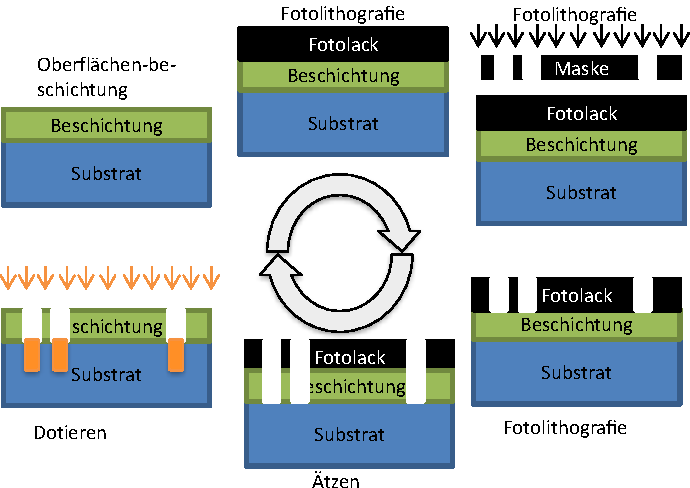
\includegraphics[width=\columnwidth, align=t]{images/01_technologie_grundprozess_skript.pdf}
\end{minipage}
\hfill
\begin{minipage}[t]{0.48\columnwidth}
    \paragraph{Lithographie}
    Lichtempfindlicher Lack (Photoresist) wird durch eine Lichtquelle löslich (positiver Photoresist) oder unlöslich (negativer Photoresist) gemacht.
    Durch Lösen des löslichen Photoresists kann die Oberfläche lokal geschützt werden und so gezielt regionen des Chips geätzt oder beschichtet werden.
    Zum Ende wird der übrige Lack entfernt und der Vorgang beliebig oft wiederholt.
\end{minipage}


% \paragraph{Lithographie}
% Das Prinzip der Lithographie basiert auf einem lichtempfindlichen Lack, dem sogenannten Photoresist.
% Dieser wird durch eine Lichtquelle löslich (positiver Photoresist) oder unlöslich (negativer Photoresist) gemacht.
% Durch lösen des löslichen Photoresists kann die Oberfläche lokal geschützt werden und so gezielt regionen des Chips geätzt oder beschichtet werden.
% Zum Ende wird der übrige Lack entfernt und der Vorgang beliebig oft wiederholt.


\paragraph{Ätzen}
Durch Ätzen kann gezielt Material von freiliegenden Flächen des Wafers entfernt werden.
Dabei werden folgende Verfahren unterschieden:
\begin{description}
    \item[Isotrop (Nass oder Plasma):] Gleichförmiges Ätzen in alle Richtungen \rightarrow Bringt die Gefahr des Unterätzens
    \item[Anisotrop (Reactive Ion Etching, KOH oder Plasma):] Ätzen entlang Kristallrichtungen, z.B. KOH greift die (111)-Ebene kaum an \rightarrow Ermöglicht steiliere Gräben, MEMS
    \item[Selektiv:] Selektives Ätzen bestimmter Materialien, z.B. HF ätzt SiO$_2$ aber nicht Si \\
        \rightarrow Erlaubt das Ätzen einer Lage ohne beschädigung unterliegender Strukturen
\end{description}

\paragraph{Dotieren}
Beim Dotieren werden gezielt Fremdatome in den Siliziumkristall eingebracht.
\begin{description}
    \item[Donatoren,] also Atome mit einem Valenzelektron mehr als der Halbleiter, verursachen einen Elektronenüberschuss, der Kristall wird \textbf{n-dotiert}.
    \item[Akzeptoren,] also Atome mit einem Valenzelektron weniger als der Halbleiter, verursachen einen Lochüberschuss, der Kristall wird \textbf{p-dotiert}.
\end{description}


\subsubsection{Backend Prozesse}

\paragraph{Wafer Sort}
Die Chips werden auf dem Wafer einzeln getestet (Kontaktierung mit Nadeln). 
Dies ist oft zeitaufwendig \rightarrow Durch gutes Design sollte diese Zeit minimiert werden.

Der Yield, (prozentualer Anteil funktionaler Chips) hängt dabei von der Chipgrösse ab.
Dies, da jeder Defekt bei grossen Chips eine grosse Fläche beeinträchtigt, da jeweils nur ganze Chips funktionsfähig oder defekt sein können.

Yields von \qty{90}{\percent} sind meist notwendig, um Profit zu machen.

\paragraph{Assembly and Test}
Die Wafer werden in einzelne Chips getrennt und die funktionierenden Chips in Gehäuse verbaut. Im Gehäuse erfolgt ein Final-Test.


\subsection{Arten von Toleranzen}
Bei der Herstellung von Wafern werden verschiedene Toleranzen unterschieden:
\begin{description}
    \item[Devicetoleranz] Toleranzen betreffend der Strukturen auf gleichem Chip
    \item[Prozesstoleranzen] Toleranzen betreffend der Strukturen auf einem Wafer
    \item[Lostoleranz] Toleranzen innerhalb eines Batches bzw. Los (meist 25, selten bis 50 Wafer)
\end{description}

\subsection{CMOS Bauelemente}
Mögliche Strukturen und Elemente wie auch die Materialeigenschaften werden im \textbf{Technologiehandbuch} gegeben.


\subsubsection{Bipolartransistoren}
\begin{center}
    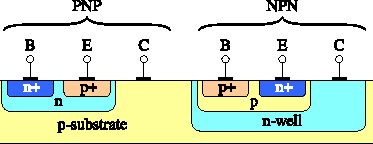
\includegraphics[width=0.5\columnwidth, align=t]{images/01_BJT.pdf}
\end{center}


\subsubsection{Kapazitäten (pro Fläche)}

\vspace{-0.3cm}

\[ 
    \boxed{ C = \varepsilon \cdot  \frac{A}{d} = \varepsilon_0 \cdot \varepsilon_r \cdot \frac{W \cdot L}{d} =  C'' \cdot A } \qquad \qquad
    \boxed{ C'' = \frac{\varepsilon}{d} = \frac{\varepsilon_0 \cdot \varepsilon_r}{d} }
\]

\begin{minipage}[t]{0.44\columnwidth}
    \begin{tabular}{l@{}}
        $\varepsilon_0 = \qty{8.85e-12}{\farad\per\meter}$                      \\
        $\varepsilon_{r, \text{Si, SiO$_2$}} \approx 3.9$                       \\
        $\varepsilon_{r, \text{Dielektrikum}} \approx 2.9$ (möglichst klein)   
    \end{tabular}   
\end{minipage}
\hfill
\begin{minipage}[t]{0.55\columnwidth}
    \begin{tabular}{lll@{}}
        $C''$   & Spezifische Kapazität & $[C''] = \qty{}{\farad\per\square\meter}$ \\
        $A$     & Fläche der Kapazität  & $[A] = \qty{}{\square\meter}$             \\
        $d$     & Abstand (fix)         & $[d] = \qty{}{\meter}$
    \end{tabular}
\end{minipage}


% \[
%     \epsilon_0 = \qty{8.85e-12}{\farad\per\meter}
% \]
% \[
%     \epsilon_{r, \text{Si, SiO$_2$}} \approx 3.9
% \]
% \[
%     \epsilon_{r, \text{Dielektrikum}} \approx 2.9 \text{\ (Typisch, so klein wie möglich)}
% \]
% \[
%     C''\text{: Spezifische Kapazität}
% \]

\paragraph{MIM}
Metal-Interconnect-Metal-Kondensatoren produzieren \textbf{sehr kleine Kapazitäten}, da die Interconnect-Layers relativ dick sind ($d \sim \qty{2.5e-7}{\meter}$) und absichtlich aus 'schlechtem' Dielektrikum ($\varepsilon_r \approx 2.9$) bestehen.
Die Spannungsfestigkeit ist jedoch höher.

\paragraph{MOS}
Da Oxidschichten sehr dünn realisiert werden können ($d \sim \qty{2.33e-9}{\meter}$) und ein höheres $\varepsilon_r \approx 3.9$ besitzen, benötigen MOS-Kondensatoren im Vergleich zu MIM-Kondensatoren bedeutend weniger Fläche.
Somit können grössere Kapazitäts-Werte realisiert werden.
Sie besitzen jedoch eine kleinere Spannungsfestigkeit.


\subsubsection{Spulen}
Spulen sind nur planar möglich und beanspruchen oft viel Platz.


\subsubsection{Widerstände (pro quadr. Flächeneinheit)}

\begin{minipage}[c]{0.44\columnwidth}
    \[ \boxed{ R = \rho \frac{L}{A} = \rho \frac{L}{t \cdot W} = R_\square \frac{L}{W} = R_\square \cdot n_\square } \]
    \[ \boxed{ R_\square = \frac{\rho}{t} } \]
\end{minipage}
\hfill
\begin{minipage}[c]{0.54\columnwidth}
    \paragraph{Typische Werte}

    \resizebox{\columnwidth}{!}
    {
    \begin{tabular}{@{}l l@{}}
            Metall              & $R_\square \approx 0.02 \dots \qty{0.08}{\ohm}/\square$                           \\
            Poly (salicide)     & $R_\square \approx \qty{10}{\ohm}/\square$                                        \\
            Poly (non-salicide) & $R_\square \approx \qty{100}{\ohm}/\square$ (n+ Poly)                             \\
                                & $R_\square \approx \qty{400}{\ohm}/\square$ (p+ Poly)                             \\
            n- / p-Diffusion    & $R_\square \approx \qty{100}{\ohm}/\square$ \, / \,  $\qty{150}{\ohm}/\square$    \\
            n- / p-Well         & $R_\square \approx \qty{400}{\ohm}/\square$ \, / \,  $\qty{1600}{\ohm}/\square$   \\
        \end{tabular}
    }
\end{minipage}


% \begin{center}
%     \boxed{
%         R = \rho \frac{L}{A} = \rho \frac{L}{t \cdot W} = R_\square \frac{L}{W}
%     }
% \end{center}
% \begin{center}
%     \boxed{
%         R_\square = \frac{\rho}{t}
%     }
% \end{center}


\subsubsection{Parasitäre Effekte}

Jedes Bauteil ist von parasitären Effekten betroffen. 
Diese sind:
\begin{itemize}
    \item Streukapazitäten und ungewollte Kapazitäten zu anderen Layern
    \item Wiederstandsbelag des Leitermaterials
    \item Induktivitätsbelag von 'langen' Leitern
    \item Toleranzen
    \item Nichtlinearitäten z.B. die Spannungsabhängigkeit der Kapazitäten von PN-Übergängen
\end{itemize}

\smallskip

\textbf{\rightarrow\ Empfehlung: Verhältnisse verwenden, nicht Absolutwerte!}


        \section{MOS Transistoren}

\subsection{Dotierung}
\begin{center}
    \begin{tabular}{lll}
        \textbf{Dotierung:}          & N-dotiert            & P-dotiert \\
        \textbf{Unreinheit:}         & Aluminium (HG III)   & Phosphor / Arsen (HG V) \\
        \textbf{Majoritätsträger:}   & Elektronen           & Löcher \\
        \textbf{Minoritätsträger:}   & Löcher               & Elektronen \\
    \end{tabular}
\end{center}


\subsection{MOS-Kapazität}
\begin{minipage}[t]{0.5\columnwidth}
    Minoritätsträger werden an das Gate gezogen.
    Die entstandene Raumladungszone weist bei ausreichend hoher Gate-Spannung einen Minoritätsträgerüberschuss auf, ist also in der Funktion \textbf{komplementär} zum Substrat dotiert.
\end{minipage}
\hfill
\begin{minipage}[t]{0.48\columnwidth}
    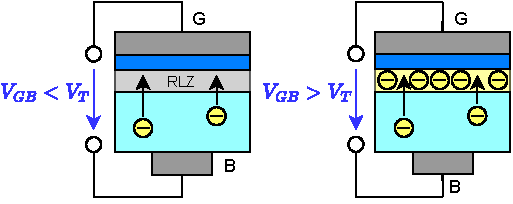
\includegraphics[width=\columnwidth, align=t]{images/02_MOS_kapazitaet.pdf}
\end{minipage}


\subsection{MOS-Transistoren}
Werden links und rechts vom MOS-Kondensator komplementär zum Substrat dotierte Regionen (Drain und Source) erstellt, so kann ohne Gatespannung aufgrund der PN-Übergänge kein Strom vom Drain zur Source (oder umgekehrt) fliessen.
Wird nun eine Spannung am Gate angelegt, so entsteht die Minoritätsträger-Leitende Raumladungszone - der Kanal.
Dieser verbindet Drain und Source, es kann also ein Strom fliessen.

\vspace{-0.2cm}

\begin{center}
    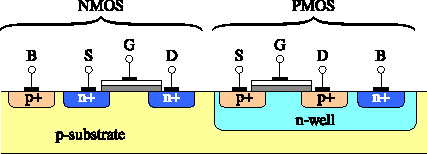
\includegraphics[width=0.5\columnwidth, align=t]{images/02_CMOS.pdf}
\end{center}


\subsubsection{Übersicht und Symbole}

\begin{minipage}[t]{0.48\columnwidth}
    Durch Vordotierung des Kanals kann der Transistor ohne Gate-Spannung leitend gemacht werden (Verarmungstyp, selbstleitend).
    Eine negative Gate-Spannung kann den Kanal dann abschnüren. \\
    \rightarrow\ hier nicht weiter behandelt

    \smallskip

    \textbf{Der Bulk wird nur eingezeichnet, wenn dieser \myul{nicht} mit $\bm{V_{\rm DD}}$ bzw. $\bm{V_{\rm SS}}$ verbunden ist.}
    Deshalb werden meist die vereinfachten Symbole verwendet:

    \vspace{-0.3cm}

    \begin{center}
        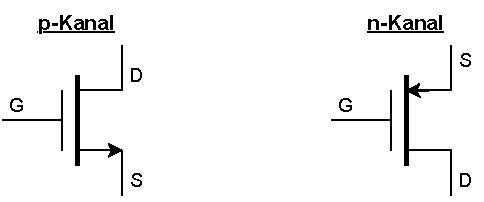
\includegraphics[width=0.8\columnwidth, align=t]{images/02_MOSFET_symbole_vereinfacht.pdf}
    \end{center}
\end{minipage}
\hfill
\begin{minipage}[t]{0.5\columnwidth}
    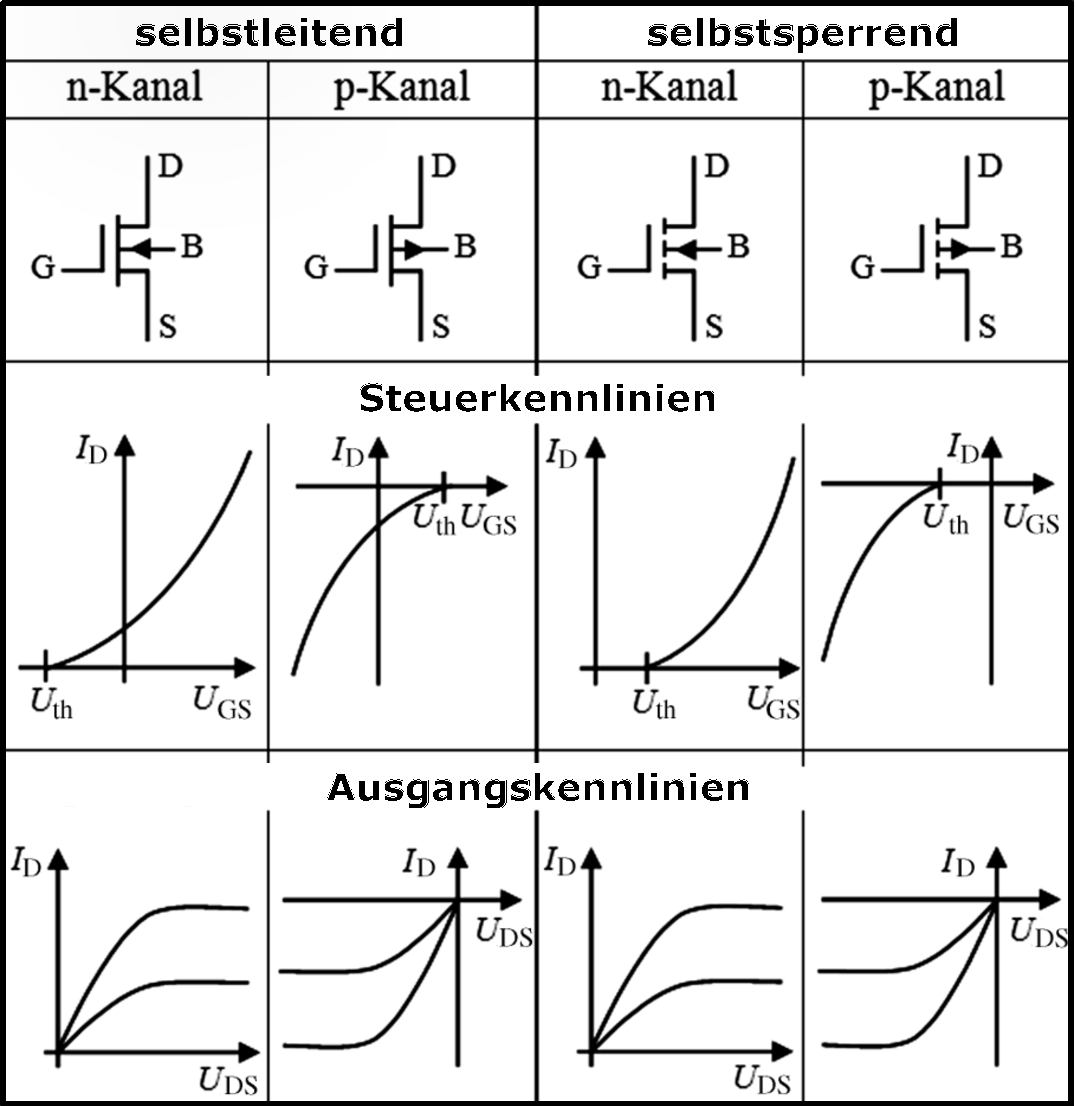
\includegraphics[width=\columnwidth, align=t]{images/02_MOSFET_uebersicht.pdf}
\end{minipage}



\subsubsection{Modelle}
In Cadence sind verschiedene Modelle hinterlegt:

\textbf{Spice Modell 11:} Das Modell 11 beinhaltet ca. 100 Parameter und ist entsprechend genau.

\textbf{Spice Modell 1:} Vergleichbar mit dem Handrechenmodell, welches zwar weniger genau, dafür aber viel einfacher ist. Dennoch beinhaltet es bereits 40 Parameter.

\subsection{Ausgangskennlinie -- Arbeitsbereiche}
 
Die Ausgangskennlinie beschreibt den Zusammenhang $I_D = f(V_{DS}) \big|_{V_{GS} = \text{konst}}$

\begin{minipage}[t]{0.5\columnwidth}
    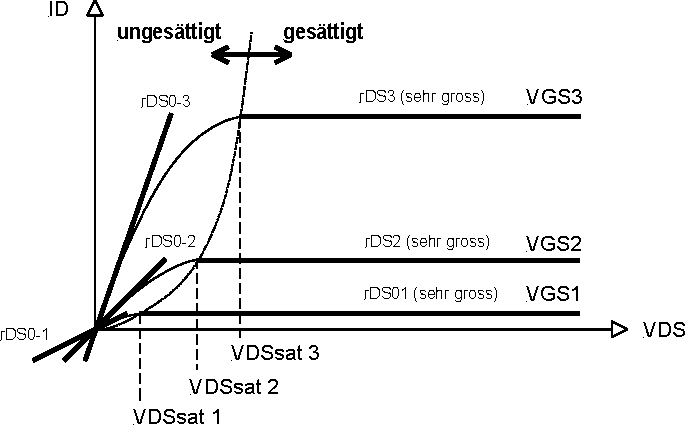
\includegraphics[width=\columnwidth, align=t]{images/02_MOSFET_ausgangskennlinien.pdf}
\end{minipage}
\hfill
\begin{minipage}[t]{0.48\columnwidth}
    Zwei Arbeitsbereiche: 

    \begin{outline}
        \1 ungesättig (gesteuerter Widerstand)
        \1 gesättigt (Stromquelle)
    \end{outline}

    \medskip

    Die Sättigungsgrenze $V_{\rm DS, sat}$ ist abhängig vom \textbf{Kanalzustand}:

    \begin{outline}
        \1 \textbf{weak inversion:} \\
            $V_{\rm DS, sat} = V_{\rm eff} \approx 5 \cdot V_{\rm temp} \approx \qty{130}{\milli \volt}$ 
        \1 \textbf{strong inversion:} \\
            $V_{\rm DS, sat} = V_{\rm eff} = V_{GS} - V_T$ 
    \end{outline}
\end{minipage}



\subsection{Transferkennlinie -- Ausgangsstrombereiche}


\begin{minipage}[t]{0.55\columnwidth}
    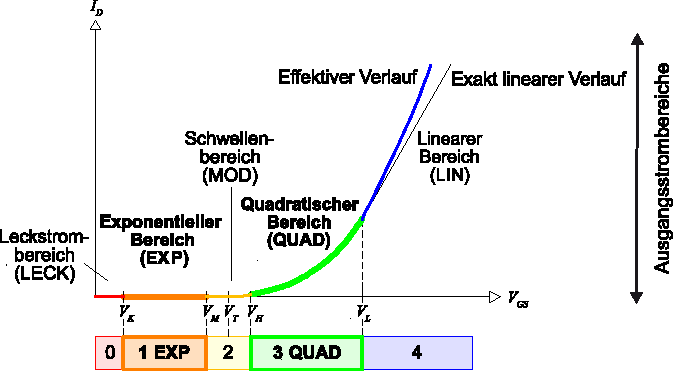
\includegraphics[width=\columnwidth, align=t]{images/02_MOSFET_transferkennlinie.pdf}
\end{minipage}
\hfill
\begin{minipage}[t]{0.42\columnwidth}
    Die Transferkennlinie beschreibt den Zusammenhang $I_D = f(V_{GS})$ 

    \smallskip

    Dabei werden \textbf{5 Ausgangsstombereiche} unterschieden. Diese hängen mit dem \textbf{Kanalzustand} zusammen.

    \smallskip

    Des Weiteren gibt es die Bereiche:

    \begin{outline}
        \1 Sub Threshold: $V_{GS} < V_T$
        \1 Above Threshold: $V_{GS} > V_T$
    \end{outline}
\end{minipage}


\para{Ausgangsstrombereiche}

\scalebox{0.8}{
\begin{tabular}{|l|l|l|}
    \hline
    \textbf{Bereich}                    & \textbf{Mathem. Charakterisierung}            & \textbf{Zugrundeliegender phys. Effekt}                       \\  
    \hline
    \rowcolor[HTML]{F4CCCC} 
    LECK                                & $I_D$ erreicht Minimalwert, der nicht         & Drain- und Source-Substratdiode haben                         \\
    \rowcolor[HTML]{F4CCCC} 
                                        & weiter unterschritten werden kann             & Leckströme ins Subsstrat                                      \\
    \hline
    \rowcolor[HTML]{FFE5BB} 
    EXP                                 & $I_D$ steigt exponentiell mit $V_{GS}$        & Kanal zeigt \textbf{weak inversion}                           \\
    \hline
    \rowcolor[HTML]{FFF2CC} 
    MOD                                 & Keine 'handliche' Formel für $I_D$            & Kanal zeigt \textbf{moderate inversion}                       \\
    \hline
    \rowcolor[HTML]{D9EAD3} 
    QUAD                                & $I_D$ steigt quadratisch mit $V_{GS}$         & Kanal zeigt \textbf{strong inversion}                         \\
    \hline
    \rowcolor[HTML]{CFE2F3} 
    LIN                                 & $I_D$ steigt annähernd linear mit $V_{GS}$    & Geschwindigkeitssättigung der Ladungsträger im Kanal          \\
    \rowcolor[HTML]{CFE2F3} 
                                        & (halb QUAD, halb LIN)                         & im Kanal (nicht weiter beschleunigbar)                        \\
    \hline
\end{tabular}
}

\smallskip

\textbf{Hinweis:} Die Inversion des Kanals beschreibt, wie sehr sich die Polarität geändert ('invertiert') hat. 
Bei einem n-Kanal FET ist der Kanal ursprünglich p-leidend.
Wird der Kanal invertiert, so wird er (schwach, moderat oder start) n-leitend. 

%NOTE [Simi] Kommt später bei Pi-Ersatzschaltung verallgemeinert dran und ist daher hier auskommentiert
% \subsection{Ersatzschaltungen}

% Je nach Arbeitsbereich (gesättigt / ungesättigt) müssen verschiedene Ersatzschaltungen verwendet werden.

% \begin{minipage}[t]{0.48\columnwidth}
%     \raggedright

%     \subsubsection*{Ungesättigt}

%     Gesteuerter Widerstand \rightarrow\ $I_D = f(V_{DS})$
    
%     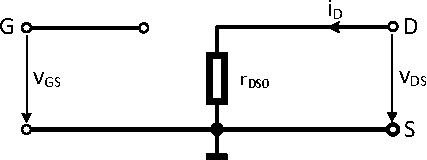
\includegraphics[width=\columnwidth, align=t]{images/02_MOSFET_ersatzschaltung_ungesaettigt.pdf}

%     \smallskip
%     Je kleiner $r_{\rm DS0}$, desto steiler die Geraden links im Ausgangskennlinienfeld

% \end{minipage}
% \hfill
% \begin{minipage}[t]{0.48\columnwidth}
%     \raggedright

%     \subsubsection*{Gesättigt}

%     Stromquelle \rightarrow\ $I_D = f(V_{GS})$

%     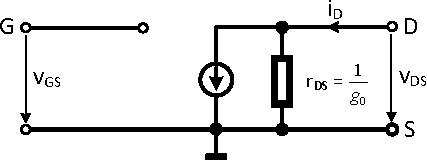
\includegraphics[width=\columnwidth, align=t]{images/02_MOSFET_ersatzschaltung_gesaettigt.pdf}

%     \smallskip
%     Je grösser $r_{\rm DS}$, desto flacher die Geraden rechts im Ausgangskennlinienfeld
% \end{minipage}


\subsection{Berechnung des Drainstroms}

Die Berechnung des Drainstroms hängt sowohl von Arbeitsbereich (gesättigt / ungesättig), als auch vom Ausgangsstrombereich (bzw. der Kanaliversion) ab!


\subsubsection{Strong Inversion}
\label{Strong Inversion}

\vspace{-0.3cm}

% $$ \boxed{ \text{QUAD-Bereich: } V_H(I_D) < V_{GS} < V_L(I_D) } \qquad \qquad \beta = \mu \cdot C_{\text{OX}} \cdot \frac{W}{L} $$
\[ \boxed{ \text{QUAD-Bereich:} \quad |V_H(I_D)| \leq |V_{GS}| < |V_L(I_D)| \quad \text{bzw.} \quad |I_H'| \leq |I_D'| < |I_L'| } \]  %NOTE: Bedingung für Ströme aus Ü3, 3.6.4 1)

\resizebox{\columnwidth}{!}
{
    \renewcommand{\arraystretch}{1.5}
    \begin{tabular}{@{}l c | c@{}}
                & \textbf{Ungesättigt:} \quad $\bm{| V_{DS} | < | V_{GS} - V_T |}$                                                              & \textbf{Gesättigt:} \quad $\bm{| V_{DS} | \geq | V_{GS} - V_T |}$                         \\
        NMOS:   & $I_D = \beta \cdot \bigg[ (V_{GS} - V_T) V_{DS} - \frac{V_{DS}^2}{2} \bigg] \cbl{\cdot (1 + \lambda \cdot \Delta V_{DS})}$    & $I_D = \frac{\beta}{2} (V_{GS} - V_T)^2 \cbl{\cdot (1 + \lambda \cdot \Delta V_{DS})}$    \\
        \midrule
        PMOS:   & $I_D = - \beta \cdot \bigg[ (V_{GS} - V_T) V_{DS} - \frac{V_{DS}^2}{2} \bigg] \cbl{\cdot (1 - \lambda \cdot \Delta V_{DS})}$  & $I_{D} = - \frac{\beta}{2} (V_{GS} - V_T)^2 \cbl{\cdot (1 - \lambda \cdot \Delta V_{DS})}$
    \end{tabular}
    \renewcommand{\arraystretch}{1}
}

\medskip

\textbf{Ohne} Berücksichtigung der \textbf{Kanallängenmodulation:} \cbl{blauen Term $=1$} bzw $\lambda = 0$ setzen



% NOTE [Simi] @Flurin: Hier noch dein Vorschlag der Darstellung (mit NMOS / PMOS Ergänzung):
% Jetzt können wir streiten, welchen wir nehmen wollen :P

% \resizebox{\columnwidth}{!}
% {
%     \renewcommand{\arraystretch}{1.5}
%     \begin{tabular}{l c|c}
%                 & \textbf{Ungesättigt:} \quad $\bm{| V_{\rm DS} | < | V_{GS} - V_T |}$                          & \textbf{Gesättigt:} \quad $\bm{| V_{\rm DS} | \geq | V_{GS} - V_T |}$             \\
%         NMOS:   & $I_{\rm D, ideal} = \beta \cdot \bigg[ (V_{GS} - V_T) V_{DS} - \frac{V_{DS}^2}{2} \bigg]$     & $I_{\rm D, ideal} = \frac{\beta}{2} (V_{GS} - V_T)^2 $                            \\
%         NMOS:   & $I_{\rm D, real} = I_{\rm D, ideal} \cdot (1 + \lambda \cdot \Delta V_{DS})$                  & $I_{\rm D, real} = I_{\rm D, ideal} \cdot (1 + \lambda \cdot \Delta V_{DS})$      \\
%         \midrule
%         PMOS:   & $I_{\rm D, ideal} = - \beta \cdot \bigg[ (V_{GS} - V_T) V_{DS} - \frac{V_{DS}^2}{2} \bigg]$   & $I_{\rm D, ideal} = - \frac{\beta}{2} (V_{GS} - V_T)^2$                           \\
%         PMOS:   & $I_{\rm D, real} = I_{\rm D, ideal} \cdot (1 - \lambda \cdot \Delta V_{DS})$                  & $I_{\rm D, real} = I_{\rm D, ideal} \cdot (1 - \lambda \cdot \Delta V_{DS})$      
%     \end{tabular}
%     \renewcommand{\arraystretch}{1}
% }



\paragraph{Transkonduktanz-Parameter $\bm{\beta}$}

\begin{minipage}[c]{0.78\columnwidth}
    $\beta$ ist abhängig davon, ob der Transistor gesättigt ist. 
    In der Praxis wird diese Unterscheidung jedoch \textbf{nicht} gemacht. 
    Im \textbf{Design} kann $\beta$ durch das Verhältnis von Kanalbreite $W$ und -länge $L$ beeinflusst werden.
\end{minipage}
\hfill
\begin{minipage}[c]{0.2\columnwidth}
    \[ \beta = \underbrace{ \mu C_{\rm OX} }_{\beta_0} \frac{W}{L} \]
\end{minipage}


%TODO: [Flurin] NMOSI und PMOSI V2S12
% NOTE: [Simi] @ Flurin: Bist du sicher, dass du diese Slide meinst...? 



%TODO: [Flurin] V3S9 nochmal studieren, macht iwie noch nicht so sinn.
\paragraph{Kanallängenmodulation $\bm{\lambda$} und Early-Spannung $\bm{V_E}$}

% Die Early-Spannung $V_E = a_E \cdot L$ setzt sich zusammen aus dem technologieabhängigen Early-Faktor $a_E$ und der Kanallänge $L$.
Die Kanallängenmodulation beschreibt die Nichtidealität der spannungsgesteurten Stromquelle (im Sättigungsbetrieb).

$$ \lambda = \frac{1}{V_E + V_{DS, \rm sat}} \approx \frac{1}{V_E} \approx \frac{1}{a_E \cdot L} \qquad \text{Idealfall: } \lambda = 0 \text{ \rightarrow\ } L = \infty $$ 

\textbf{Achtung:} $\bm{V_E}$ ist typischerweise negativ, wird jedoch \textbf{immer positiv angegeben}. 
Grafisch entspricht $V_E$ der Spannung $V_{DS}$, bei welcher die Verlängerung der Ausgangskennlinie (Sättigung) die $V_{DS}$-Achse schneidet.


%CHECK: [Flurin] Ich finde die Herleitung aus V3S9 überflüssig. Evtl. macht die Grafik zur Early-Spannung sinn? Braucht halt viel platz...
% [Simi] @Flurin: Ja, auf die Herleitung würde ich auch verzichten. Das Bild wäre allenfalls sinnvoll. 
% Aus Platzgründen habe ich etws 'Prosa' zur Early-Spannung geschrieben... Wirklich toll ist der Text aber auch nicht...


\paragraph{Body-Effekt}
Der Body-Effekt beschreibt die \textbf{Abhängigkeit der Schwellenspannung} $\bm{V_T}$ von der Source-Bulk-Spannung $V_{SB}$ als
\[ 
    V_T = V_{T0} \pm \Delta V_T 
    \quad \text{mit} \quad 
    \Delta V_T = \gamma\left(\sqrt{\abs{V_{SB}} + \abs{2\Phi_F}}-\sqrt{\abs{2\Phi_F}}\right)
\]

\rightarrow\ \textbf{Body-Effekt nur wirksam, wenn} $\mathbf{V_{SB} \neq \qty{0}{\volt}}$ \\
\rightarrow\ Reminder: Bulk nur gezeichnet, wenn nicht auf $V_{DD}$ oder $V_{SS}$

\medskip

Das Fermi-Potential $\Phi_F$ ist prozess- wie auch temperaturabhängig. Zudem ist es abhängig von der Dotierungsstärke.

%NOTE: [Simi] Wenn kein Platz: folgende Tabelle weglassen (diese Formeln sind uns gemäss Zbinden egal)
\begin{minipage}[c]{0.3\columnwidth}
    \[ \Phi_F = \frac{kT}{q} \ln \left( \frac{N_A}{n_i} \right) \]
    \[ \gamma_N \overset{n-Dotierung}{\approx} \qty{1.46}{\sqrt{\volt}} \]
    \[ \gamma_P \overset{p-Dotierung}{\approx} \qty{1.08}{\sqrt{\volt}} \]
\end{minipage}
\hfill
\begin{minipage}[c]{0.68\columnwidth}
    \begin{tabular}{rl}
        $n_i$       & Intrinsische ladungsdichte von Silizium   \\
        $N_A$       & Ladungsdichte der Akzeptoren              \\
        $\gamma$    & Body-Effekt-Konstante                     \\
        $T$         & \textbf{Absolute} Temperatur              \\
        $k$         & Boltzmann-Konstante $\qty{1.380649 e-23}{\joule\per\kelvin}$  \\
        $q$         & Elementarladung $\qty{1.602 e-19}{\coulomb}$
    \end{tabular}
\end{minipage}


\subsubsection{Weak Inversion}

\vspace{-0.3cm}

% $$ \boxed{ \text{EXP-Bereich: } V_K(I_D) < V_{GS} < V_M(I_D) \qquad \qquad V_M(I_D) = V_T(I_D) - x_M(I_D) } $$
\[ \boxed{ \text{EXP-Bereich: } |V_K(I_D)| < |V_{GS}| \leq |V_M(I_D)| \quad \text{bzw.} \quad |I_K'| < |I_D'| \leq |I_M'| } \]  %NOTE: Bedingung für Ströme aus Ü3, 3.6.5 1)


\resizebox{\columnwidth}{!}
{
    \renewcommand{\arraystretch}{1.5}
    \begin{tabular}{@{}l c | c@{}}
                & \textbf{Ungesättigt:} \quad $\bm{| V_{DS} | < | V_{GS} - V_T |}$                                                                                                  & \textbf{Gesättigt:} \quad $\bm{| V_{DS} | \geq | V_{GS} - V_T |}$                                                     \\
        NMOS:   & $I_D = I_M \cdot \e^{\frac{V_{GS} - V_M}{n_M \cdot V_\text{temp}}} \cdot (1 - \e^{-\frac{V_{DS}}{V_\text{temp}}}) \cbl{\cdot (1 + \lambda \cdot \Delta V_{DS})}$  & $I_D = I_M \cdot \e^{\frac{V_{GS} - V_M}{n_M \cdot V_\text{temp}}} \cbl{\cdot (1 + \lambda \cdot \Delta V_{DS})}$     \\
        \midrule
        PMOS:   & $I_D = I_M \cdot \e^{- \frac{V_{GS} - V_M}{n_M \cdot V_\text{temp}}} \cdot (1 - \e^{\frac{V_{DS}}{V_\text{temp}}}) \cbl{\cdot (1 - \lambda \cdot \Delta V_{DS})}$ & $I_D = I_M \cdot \e^{- \frac{V_{GS} - V_M}{n_M \cdot V_\text{temp}}} \cbl{\cdot (1 - \lambda \cdot \Delta V_{DS})}$   \\
    \end{tabular}
    \renewcommand{\arraystretch}{1}
}

\medskip

\textbf{Ohne} Berücksichtigung der \textbf{Kanallängenmodulation:} \cbl{blauen Term $=1$} bzw $\lambda = 0$ setzen





% NOTE [Simi] @Flurin: Hier noch dein Vorschlag der Darstellung (mit NMOS / PMOS Ergänzung):
% Jetzt können wir streiten, welchen wir nehmen wollen :P

% \resizebox{\columnwidth}{!}
% {
%     \renewcommand{\arraystretch}{1.5}
%     \begin{tabular}{l c|c}
%                 & \textbf{Ungesättigt:} \quad $\bm{| V_{\rm DS} | < | V_{GS} - V_T |}$                          & \textbf{Gesättigt:} \quad $\bm{| V_{\rm DS} | \geq | V_{GS} - V_T |}$                   \\
%         NMOS:   & $I_{\rm D, ideal} = I_M \cdot \e^{\frac{V_{GS} - V_M}{n_M \cdot V_\text{temp}}}$              & $I_{\rm D, ideal} = I_M \cdot \e^{\frac{V_{GS} - V_M}{n_M \cdot V_\text{temp}}}$        \\
%         NMOS:   & $I_{\rm D, real} = I_{\rm D, ideal} \cdot (1 + \lambda \cdot \Delta V_{DS})$                  & $I_{\rm D, real} = I_{\rm D, ideal} \cdot (1 + \lambda \cdot \Delta V_{DS})$            \\
%         \midrule
%         PMOS:   & $I_{\rm D, ideal} = I_M \cdot \e^{- \frac{V_{GS} - V_M}{n_M \cdot V_\text{temp}}}$            & $I_{\rm D, ideal} = - I_M \cdot \e^{- \frac{V_{GS} - V_M}{n_M \cdot V_\text{temp}}}$    \\
%         PMOS:   & $I_{\rm D, real} = I_{\rm D, ideal} \cdot (1 - \lambda \cdot \Delta V_{DS})$                  & $I_{\rm D, real} = I_{\rm D, ideal} \cdot (1 - \lambda \cdot \Delta V_{DS})$      
%     \end{tabular}
%     \renewcommand{\arraystretch}{1}
% }





%NOTE [Simi] @Flruin Würde ich gemäss aktuellem Inhalt der Zusammenfassung nicht mehr so drauf nehmen. Alle Informationen stehen weiter oben / unten
% Zu den 130 mV: Das ist eine Approximation für: V_{DS, sat} = 5 \cdot  V_{\rm temp} (siehe Abschnitt 2.4) -> das kam so im Quiz dran

% Dabei wird $V_{\rm temp}$ oft vom Technologiehandbuch gegeben. 

% Alternativ kann sie als 

% \begin{minipage}{0.4\columnwidth}
%     \[
%         V_{\rm temp} = \frac{kT}{q} \approx \qty{130}{\milli\volt}    % TODO: @Flurin: Falls das doch wieder einkommentiert wird,, 130 mV korrigieren
%     \]
% \end{minipage}
% \hfill
% \begin{minipage}{0.5\columnwidth}
%     \begin{tabular}{rl}
%         $k$: & Boltzmann-Konstante \\
%         $q$: & Elementarladung \\
%         $T$: & Temperatur in Kelvin \\
%     \end{tabular}
% \end{minipage}

% CHECK: [Flurin] Ist das tatsächlich eine approximation? Was stimmt nicht daran?
% approximativ berechnet werden.



%CHECK [Simi] @Flurin: Soll der Transkonduktanzparameter wieder rein? In der Vorlesung wurde er erwähnt, jedoch kommt er in der weak inversion Formel nicht vor...
% Ich habe ihn daher einmal auskommentiert...

\paragraph{Parameter der Formel}

\renewcommand{\arraystretch}{1.5}
\begin{tabular}{ll}
    % Transkonduktanzparameter      & $\beta = \beta_0 \frac{W}{L} = \mu C_{OX} \, \frac{W}{L}$ \\
    Temparaturspannung              & $V_{\rm temp} = \frac{k T}{q} \approx \qty{86.2}{\micro\volt\per\kelvin} \cdot T$                             \\
    (Spezifischer Drainstrom)       & $ I_M = \frac{W}{L} I_{M}' = \frac{W}{L} I_{M, 0}$                                                                                 \\
    Subthreshold Slope Factor       & $n_M = 1 + \frac{\gamma}{2\sqrt{V_{SB}+\Phi_0}}$ \quad mit \quad $\Phi_0 = 2 \Phi_F \approx \qty{0.6}{\volt}$ \\
    Kanallängenmodulation           & $\lambda = \frac{1}{V_E} \approx \frac{1}{a_E L}$
\end{tabular}
\renewcommand{\arraystretch}{1}

% \paragraph{Temparaturspannung}
% \[
%     V_{temp} = \frac{k T}{q} \approx \qty{86.2}{\micro\volt\per\kelvin} \cdot T
% \]

% \paragraph{Spezifischer Drainstrom}
% \[
%     I_M = \frac{W}{L} I_{M, 0}
% \]

% \paragraph{Subthreshold Slope Factor}
% \[
%     n_M = 1 + \frac{\gamma}{2\sqrt{V_{SB}+\Phi_0}} \quad \text{mit} \quad \Phi_0 = 2 \Phi_F \approx \qty{0.6}{\volt}
% \]

% \paragraph{Kanallängenmodulation}
% \[
%     \lambda = \frac{1}{V_E} \approx \frac{1}{a_E L}
% \]

% \paragraph{Transkonduktanz-Parameter}
% \[
%     \beta = \frac{W}{L}\beta_0 = \mu C_{OX}
% \]
% (unter Vernachlässigun
% \paragrag der Abhängigkeit von der Sättigung.)







\subsubsection{Bereiche ohne Berechnungsformeln}

In den drei verbleibenden Bereichen sind \textbf{keine Berechnungsformeln für} $\bm{I_D}$ vorhanden.

\smallskip

\begin{minipage}[c]{0.48\columnwidth}
    \renewcommand{\arraystretch}{1.2}
    \begin{ctabular}{lll}
        \textbf{Bereich}    & \textbf{Grenzen}                  \\
        LECK                & $V_K(I_D) < V_{GS} < V_M(I_D)$    \\ 
        MOD                 & $V_M(I_D) < V_{GS} < V_H(I_D)$    \\ 
                            & $V_H(I_D) = V_T(I_D) + x_H(I_D)$  \\
        LIN                 & $V_L(I_D) < V_{GS}$               \\ 
    \end{ctabular}
\end{minipage}
\hfill
\begin{minipage}[c]{0.48\columnwidth}
    Im MOD-Bereich (moderate inversion) liefern die Formeln der weak bzw. strong inversion katastrophal falsche Resultate!

    \smallskip

    Es ist daher enorm wichtig, den Arbeitsbereich des Transistors korrekt zu bestimmen.
\end{minipage}


\subsection{Modellierung eines MOS-FET in einem Arbeitspunkt}

Der Transistor ist sehr komplex.
Daher wird er \textbf{in einem Arbeitspunkt} folgendermassen vereinfacht  und modelliert:

\begin{enumerate}
    \item Definieren des Arbeitspunkts mittels \textbf{Grosssignalersatzschaltung} (\ref{Grosssignalersatzschaltung})
    \item Linearisierung im Arbeitspunkt mittels \textbf{Kleinsignalersatzschaltung} (\ref{Niederfrequenz (Pi-Ersatzschaltung)} / \ref{Kleinsignalersatzschaltung})
    \item Linearisierte \textbf{Kleinsignalparameter} bestimmen (\ref{Kleinsignalparameter}) und damit weiterrechnen
\end{enumerate}


\subsubsection{Bestimmung des Arbeitspunkts}
\label{Bestimmung des Arbeitspunkts}
Um den 'Zustand' eines MOS-FET zu bestimmen, wird wie folgt vorgegangen:

\begin{minipage}[t]{0.44\columnwidth}
    \raggedright
    \begin{enumerate}
        \item $V_{GS}$ bestimmen 
        \item Ausgangsstrombereich mittels $V_{GS}$ bestimmen \\
            $|V_{GS}| \geq |V_H|$ \rightarrow\ strong inversion \\
            $|V_{GS}| \leq |V_M|$ \rightarrow\ weak inversion
        \item $V_{DS}$ ermitteln
    \end{enumerate}
\end{minipage}
\hfill
\begin{minipage}[t]{0.54\columnwidth}
    \raggedright
    \begin{enumerate}
        \setcounter{enumi}{3}
        \item $V_{DS, \rm sat}$ ausrechnen (Strombereich beachten)  \\
            strong inversion: $V_{DS, \rm sat} = V_{GS} - V_T$  \\
            weak inversion: $V_{DS, \rm sat} \approx 5 \cdot V_{\rm temp} \approx \qty{130}{\milli \volt}$ 
        \item Ausgangsspannungsbereich durch vergleich von $|V_{DS}|$ mit $|V_{DS, \rm sat}|$ ermitteln  \\
            $|V_{DS}| < |V_{DS, \rm sat}|$ \rightarrow\ ungesättigt \\
            $|V_{DS}| > |V_{DS, \rm sat}|$ \rightarrow\ gesättigt
    \end{enumerate}
\end{minipage}


% \begin{enumerate}
%     \item $V_{GS}$ bestimmen 
%     % \item Ausgangsstrombereich (weak inversion, strong inversion, \ldots) anhand von Vergleich von $V_{GS}$ mit $V_K$, $V_M$, $V_T$, $V_H$ und $V_L$ bestimmen
%     \item Ausgangsstrombereich mittels $V_{GS}$ bestimmen \\
%         $|V_{GS}| \geq V_H$ \rightarrow\ strong inversion \\
%         $|V_{GS}| \leq V_M$ \rightarrow\ weak inversion
%     \item $V_{DS}$ ermitteln
%     \item $V_{DS, \rm sat}$ ausrechnen (Ausgangsstrombereich beachten)  \\
%         strong inversion: $V_{DS, \rm sat} = V_{GS} - V_T$  \\
%         weak inversion: $V_{DS, \rm sat} \approx 5 \cdot V_{\rm temp} \approx \qty{130}{\milli \volt}$ 
%     \item Ausgangsspannungsbereich durch vergleich von $|V_{DS}|$ mit $|V_{DS, \rm sat}|$ ermitteln  \\
%         $|V_{DS}| < |V_{DS, \rm sat}|$ \rightarrow\ ungesättigt \\
%         $|V_{DS}| > |V_{DS, \rm sat}|$ \rightarrow\ gesättigt
% \end{enumerate}


\subsubsection{Kleinsignalersatzschlatungen des FET}

\paragraph{Niederfrequenz (Pi-Ersatzschaltung)}
\label{Niederfrequenz (Pi-Ersatzschaltung)}

\begin{minipage}[t]{0.48\columnwidth}
    % 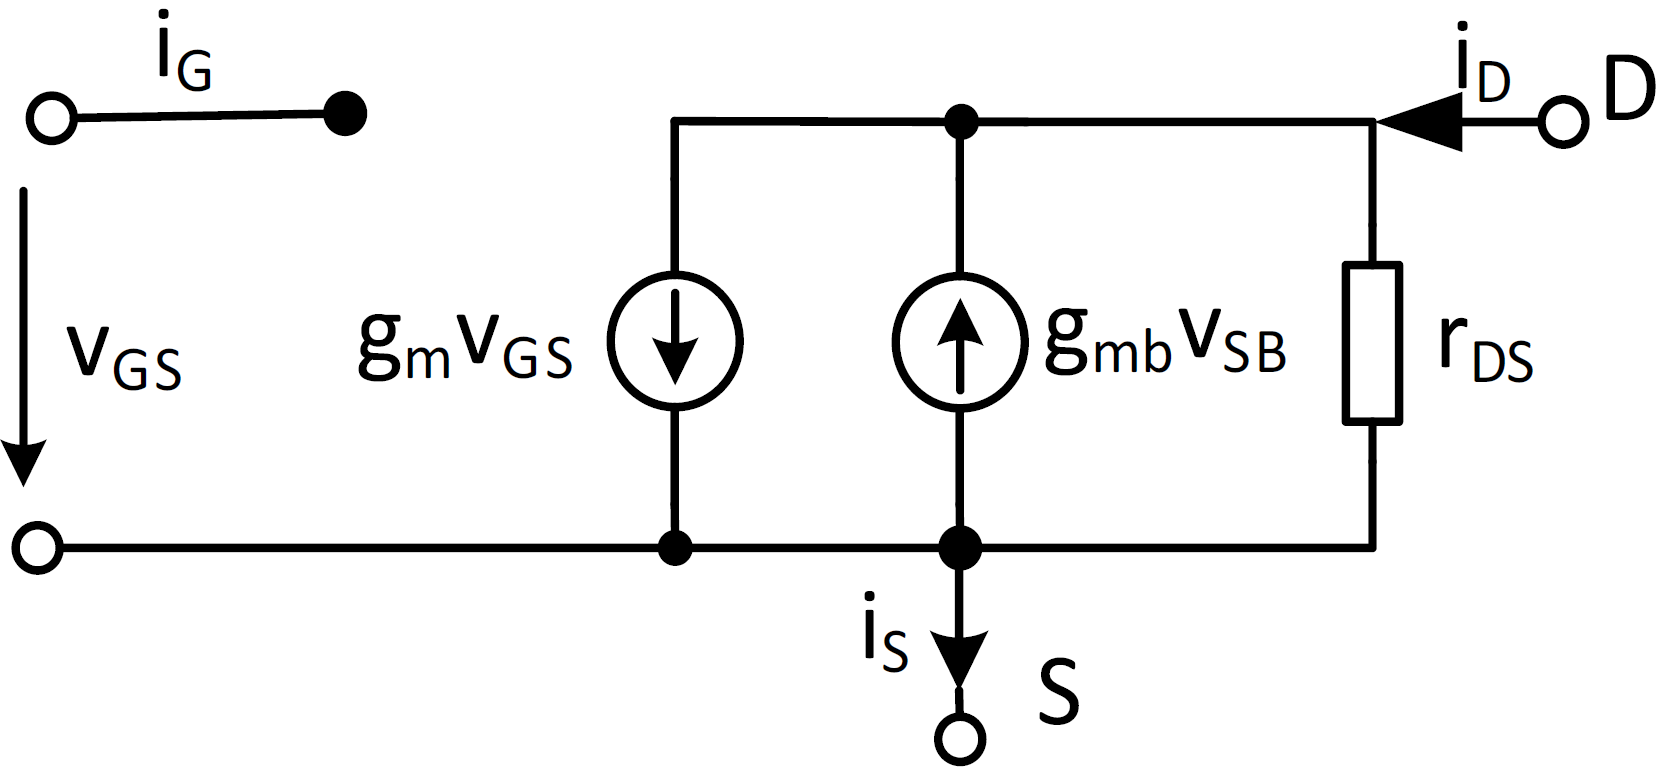
\includegraphics[width=\columnwidth, align=t]{images/02_MOSFET_Pi_Ersatzschaltung.png} Variante aus Skript
    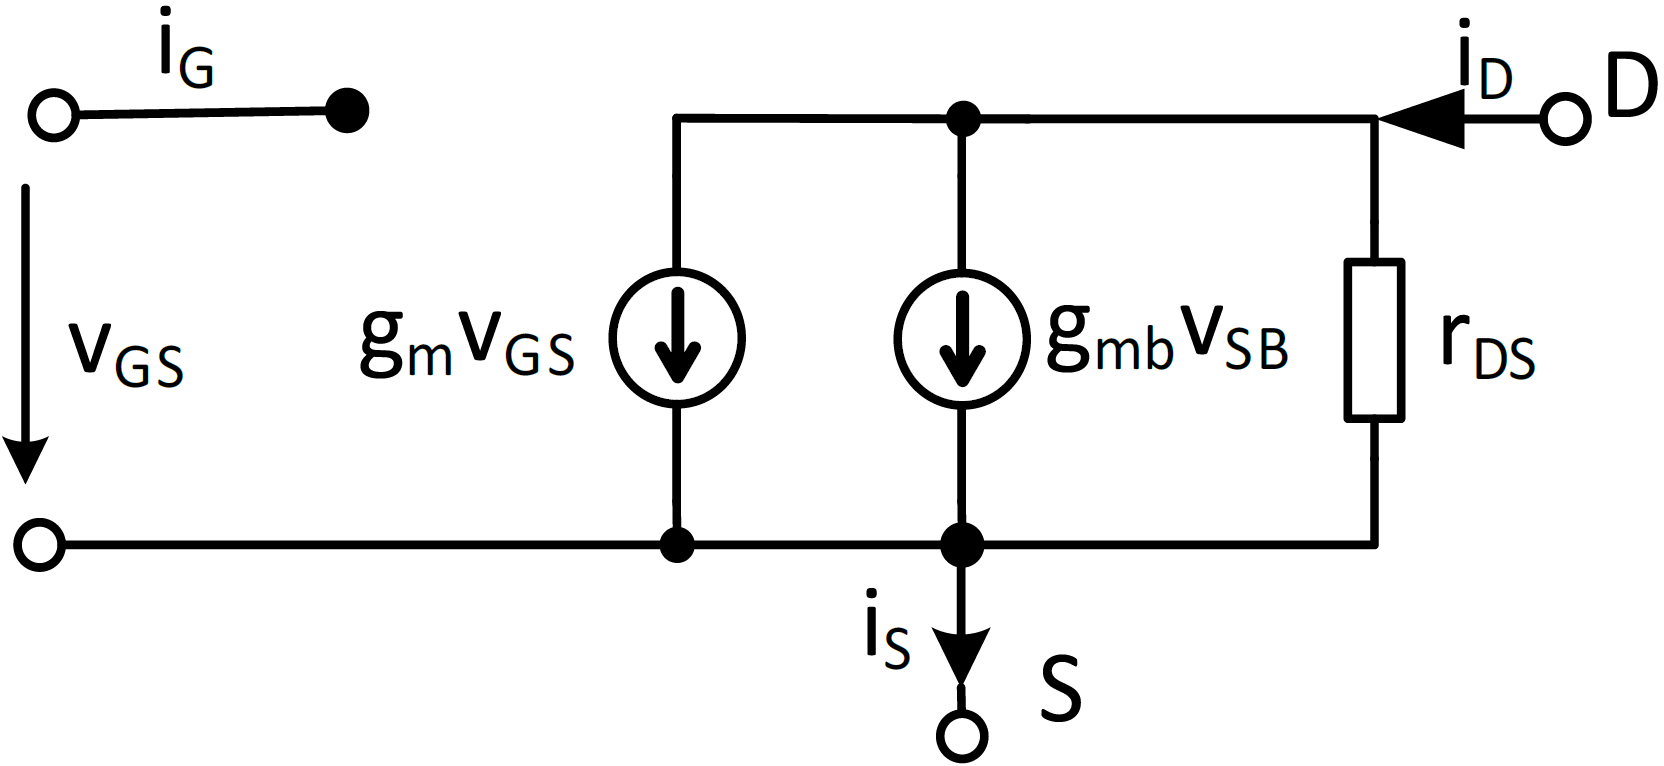
\includegraphics[width=\columnwidth, align=t]{images/02_MOSFET_Pi_Ersatzschaltung_angepasste_Stromrichtung.png}
\end{minipage}
\hfill
\begin{minipage}[t]{0.48\columnwidth}
    \raggedright
    \begin{itemize}
        \item Ideale spannungsgesteurte Stromquelle: $I_D = f(V_{GS})$
        \item Berücksichtigung von Kanallängenmodulation: $g_o$ bzw. $r_{DS}$
        \item Berücksichtigung von Body-Effekt: $g_{mb} \cdot V_{SB}$
    \end{itemize}
\end{minipage}


\paragraph{Hochfrequenz}
\label{Hochfrequenz}

\begin{minipage}[t]{0.48\columnwidth}
    % 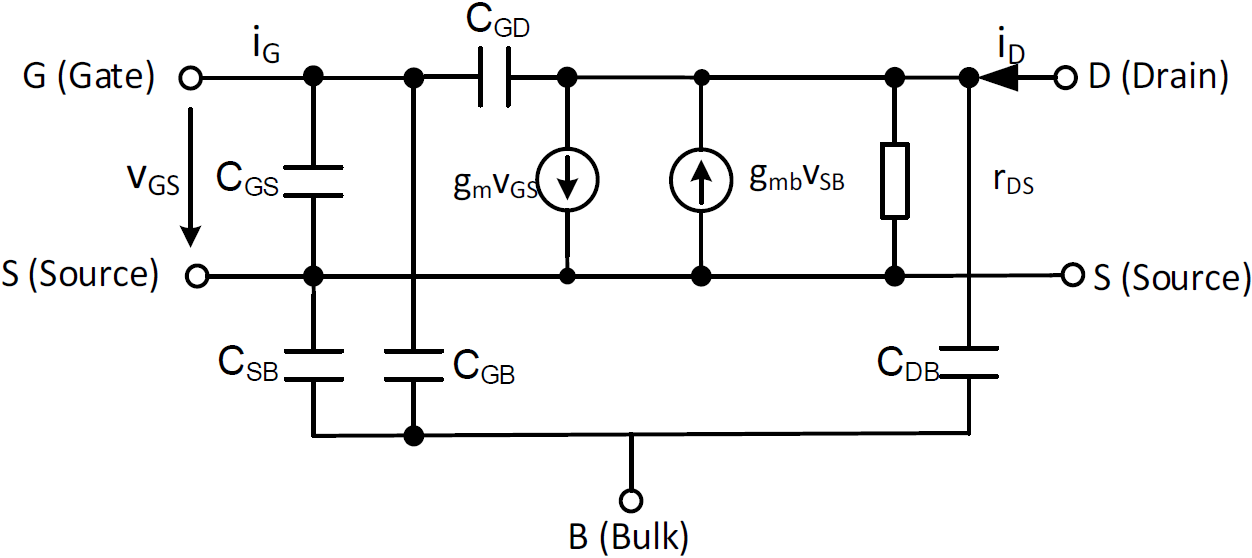
\includegraphics[width=\columnwidth, align=t]{images/02_MOSFET_Kleinsignalersatzschaltung_hochfrequent.png}   Variante aus Skript
    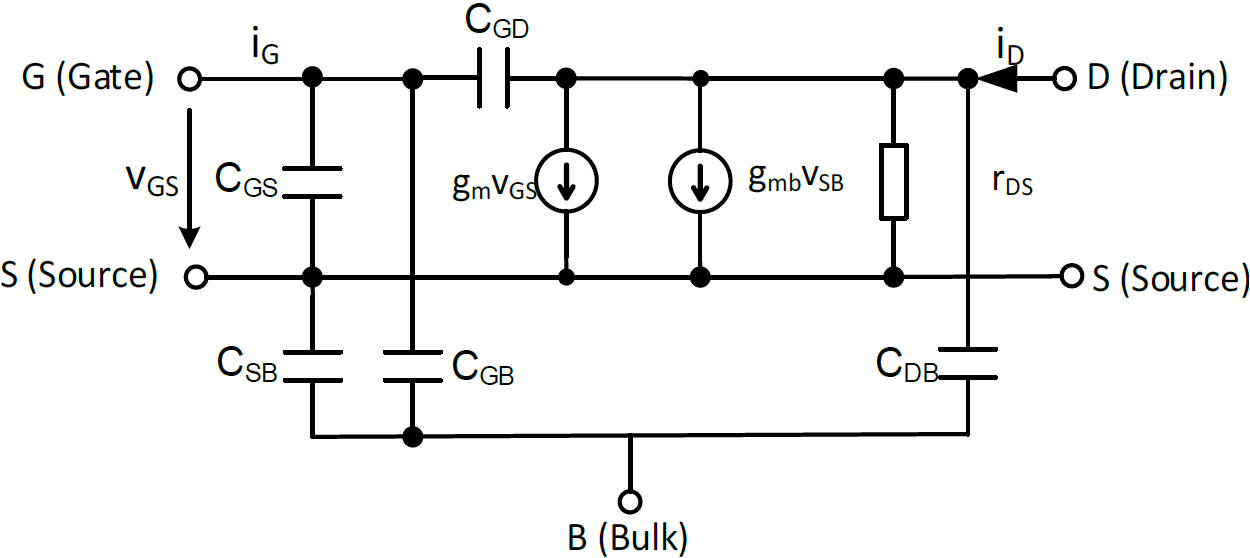
\includegraphics[width=\columnwidth, align=t]{images/02_MOSFET_Kleinsignalersatzschaltung_hochfrequent_angepasste_Stromrichtung.png}
\end{minipage}
\hfill
\begin{minipage}[t]{0.48\columnwidth}
    \raggedright
    Wenn Source und Bulk verbunden sind werden
    \begin{itemize}
        \item $C_{GB}$ und $C_{GS}$ parallel geschaltet und
        \item $C_{SB}$ kurzgeschlossen.
    \end{itemize}
\end{minipage}


\subsection{Kleinsignalparameter}
\label{Kleinsignalparameter}

Die Kleinsignalparameter bilden eine Vereinfachung (\textbf{Linearisierung}) in einem Arbeitspunkt. 
Sie berechnen sich daher allgemein folgendermassen aus der Ableitung
\[
    g_m          = \frac{\diff}{\diff V_{GS}} I_D \qquad
    g_o = r_{DS} = \frac{\diff}{\diff V_{DS}} I_D \qquad
    g_{mb}       = \frac{\diff}{\diff V_{SB}} I_D
\]

Für die beiden Kanalzustände, in welchen Formeln für die Handrechnung verfügbar sind, gibt es auch hier handliche Formeln für die Berechnung der Kleinsignalparameter.

\smallskip

Die Bezeichnung der einzelnen Parameter gilt sowohl für strong inversion als auch für weak inversion.

\medskip

\begin{tabular}{@{}ll@{}}
    $g_m$               & Transkonduktanz (Stromquellenbetrieb) \textrightarrow\ Mass für Verstärkung des Transistors   \\
    $g_{mb}$            & Body-Transkonduktanz \textrightarrow\ Beschreibt Wirkung des Body-Effekts                     \\
    $g_o$               & Ausgangsleitwert (Stromquellenbetrieb) \textrightarrow\ beschreibt Kanallängenmodulation      \\
    $r_{DS \crd{0}}$    & Kleinstmöglicher Ausgangswiderstand bzw. \textbf{Einschaltwiderstand bei} $\bm{V_{DS} = 0}$   \\
                        & \textrightarrow\ Nur im Widerstandsbetrieb interessant
\end{tabular}

\medskip

\textbf{Hinweis:} Folgende Formel gelten für nMOS Transistoren.
Für pMOS Transistoren müssen jeweils \textbf{überall Beträge eingesetzt werden} \textbf{(ausser bei Technologieparametern)} und bei Bedarf beim Gesamtresultat ein Minus ergänzt werden.


\subsubsection{Strong Inversion}

\vspace{-0.3cm}

\[
    \underbrace{ g_m = \mu C_{ox} \frac{W}{L} (V_{GS} - V_T) }_{\text{AP durch } V_{GS} \text{ bestimmt}} \qquad \qquad \qquad
    \underbrace{ g_m = \sqrt{2 \mu C_{ox} \frac{W}{L} I_D} }_{\text{AP durch } I_D \text{ bestimmt}} 
\]

% \[
%     g_{mb} = -g_m \frac{\gamma}{2 \sqrt{\abs{V_{SB}} + \abs{2 \Phi_F}}} = - g_m (n_M - 1)
% \]
% Ungesättigt:
% \[
%     g_o = \frac{1}{r_{DS}} = \mu C_{ox} \frac{W}{L} ((V_{GS} - V_T) - V_{DS})
% \]
% % Gesättigt:
% \[
%     g_o =  \frac{1}{r_{DS}} = \lambda I_{DS, sat} = \frac{I_D}{V_E + V_{DS}} \approx \frac{I_D}{a_E L + V_{DS}}
% \]

\vspace{-0.15cm}

\begin{align*}
                                         g_{mb} &= -g_m \frac{\gamma}{2 \sqrt{\abs{V_{SB}} + \abs{2 \Phi_F}}} = - g_m (n_M - 1)                                     \\
    \text{ \textbf{Ungesättigt:}} \quad     g_o &= \frac{1}{r_{DS}} = \mu C_{ox} \frac{W}{L} ((V_{GS} - V_T) - V_{DS})                                              \\
    \text{ \textbf{Gesättigt:}} \quad       g_o &=  \frac{1}{r_{DS}} = \lambda \cdot I_{DS, \rm sat} = \frac{I_D}{V_E + V_{DS}} \approx \frac{I_D}{a_E \cdot L + V_{DS}}
\end{align*}


\subsubsection{Weak Inversion}

\vspace{-0.3cm}

\[
    g_m = \frac{I_D}{n_M \cdot V_\text{temp}} \quad \text{ \textrightarrow\ Unabhängig von der Geometrie des Transistors!}
\]
% {
%     \raggedleft
%     \textrightarrow\ Unabhängig von der Geometrie des Transistors! \phantom{M}

% }

\vspace{-0.15cm}

\begin{align*}
                                         g_{mb} &= -g_m \frac{\gamma}{2 \sqrt{\abs{V_{SB}} + \abs{2 \Phi_F}}} = - g_m (n_M - 1)                                             \\
    \text{ \textbf{Ungesättigt:}} \quad     g_o &= \frac{1}{r_{DS}} = \frac{V_{\text{temp}}}{I_{D \infty}} \quad \text{ \textrightarrow\ wird meist simuliert}              \\
    \text{ \textbf{Gesättigt:}} \quad       g_o &=  \frac{1}{r_{DS}} = \lambda \cdot  I_{DS, \rm sat} = \frac{I_D}{V_E + V_{DS}}  \approx \frac{I_D}{a_E \cdot L + V_{DS}}
\end{align*}


% \[
%     g_{mb} = -g_m \frac{\gamma}{2 \sqrt{\abs{V_{SB}} + \abs{2 \Phi_F}}} = - g_m (n_M - 1)
% \]
% Ungesättigt:
% \[
%     g_o: \text{Wird üblicherweise simuliert}
% \]
% Gesättigt:
% \[
%     g_o = \frac{1}{r_{DS}} = \lambda I_{DS, sat} = \frac{I_D}{V_E + V_{DS}}
% \]

\subsection{Zusammenhänge}
%TODO: [Flurin] This seems important but I don't know how to integrate this in a logical way
% [Simi] @Flurin: Leave it here for the moment... maybe we can fit in in somewhere late or we just leave it here :) 

$g_m$ ist in der Weak Inversion unabhängig der Geometrie. 
Es ist für einen gegebenen Drainstrom möglich, Transistoren, die in Weak Inversion wie auch welche, die in Strong Inversion sind herzustellen.
Das $g_m$ steigt beim Transistor in Strong Inversion 

\subsection{Bestimmung von Ersatzschaltbildern -- Allgemein}
\subsubsection{Grosssignalersatzschaltung}
\label{Grosssignalersatzschaltung}

Zur Bestimmung des \textbf{Arbeitspunkts} bzw.\ aller Gleichspannungen.
\begin{description}
    \item[AC-Spannungsquellen] durch Kurzschlüsse ersetzen.
    \item[AC-Stromquellen] durch Unterbrüche ersetzen. 
    \item[Kondensatoren] durch Unterbrüche ersetzen.
    \item[Spulen] durch Kurzschlüsse ersetzen.  
\end{description}

\subsubsection{Kleinsignalersatzschaltung}
\label{Kleinsignalersatzschaltung}
Zur Berechnung von Verstärkungsfaktoren und Eingangswiderständen für AC-Signale.

\begin{description}
    \item[DC-Spannungsquellen] durch Kurzschlüsse ersetzen.
    \item[DC-Stromquellen] durch Unterbrüche ersetzen. 
    \item[Nichtlineare Bauteile] durch deren Kleinsignalersatzschaltbild ersetzen.
    \item[Koppel- und Bypass-Kondensatoren] durch Kurzschlüsse ersetzen.  
\end{description}


\subsection{Vorgehen: Verstärker dimensionieren}
\begin{itemize}
    \item Arbeitspunkt bestimmen.
    \item $I_D$ wählen, sodass der Transistor \textbf{gesättigt} ist.   %CHECK [Simi] @Flurin Hier stand zuvor UNgesättigt -> gemäss Beispiel von V4 S15 haben wir aber gesagt, der Transistor muss gesättigt sein...?
    \item Kleinsignalersatzschaltung zeichnen.
    \item Parameter der Ersatzschaltung bestimmen.
\end{itemize}
        \section{MOSFET Grundschaltungen}
Es werden drei Grundschaltungen unterschieden. 
Diese werden jeweils durch deren Common-Anschluss benannt.

\begin{center}
    \begingroup\rowcolors{1}{white}{gray!25}
    \begin{tabular}{|c|ccc|}
        \hline
        Schaltung   & Source-Schaltung & Gate-Schaltung & Drain-Schaltung \\
        \hline
        Common      & Source    & Gate      & Drain     \\
        Eingang     & Gate      & Source    & Gate      \\
        Ausgang     & Drain     & Drain     & Source    \\
        \hline
    \end{tabular}\endgroup
\end{center}

\textbf{Hinweis:} Die Drain-Schaltung wird auch Source-Follower genannt.


\subsection{Einsatzgebiete und Eigenschaften}

\begin{center}
    \begingroup\rowcolors{1}{white}{gray!25}
    \begin{tabular}{|c|ccc|}
        \hline
        Grundschaltung  & Anwendung                                 & $r_{\rm in}$  & $r_{\rm out}$ \\
        \hline
        Source          & Verstärker: Tiefe -- mittlere Frequenzen  & gross         & gross         \\
        Gate            & Verstärker: Hohe Freqenzen                & klein         & gross         \\
        Drain           & Spannungsfolger, Treiber, Impedanzwandler & gross         & klein         \\
        \hline
    \end{tabular}\endgroup
\end{center}

\subsection{Dimensionierung einer Grundschaltung -- Vorgehen}
\begin{easylist}
    \ListProperties(Style1*=\bfseries,Numbers2=l,Mark1={},Mark2={)},Indent2=1em)
    @ Arbeitspunkt mittels Grosssignalersatzschaltung bestimmen (\ref{Grosssignalersatzschaltung} / \ref{Bestimmung des Arbeitspunkts})
    @ Kleinsignalersatzschaltung 
    @@ Beschaltung umzeichnen
    @@ Transistor durch Ersatzschaltbild ersetzen (\ref{Kleinsignalersatzschaltung})
    @ Durch lineare Analyse Verstärkung $a$ und Ausgangswiderstand $r_{\rm out}$ berechnen
\end{easylist}

\subsection{Source-Schaltung}
\label{Source-Schaltung}

Die Source-Schaltung ist eine \textbf{invertierende Verstärkerschaltung.}

\smallskip

\begin{minipage}[t]{0.4\columnwidth}
    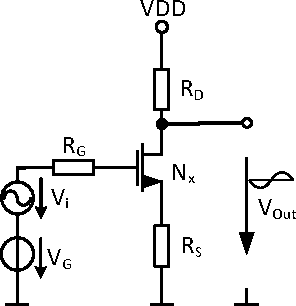
\includegraphics[width=\columnwidth, align=t]{images/03_source_schaltung.pdf}
\end{minipage}
\hfill
\begin{minipage}[t]{0.58\columnwidth}
    \subsubsection{Verstärkung}

    \vspace{-0.2cm}
    \[
        a = \frac{v_{\rm out}}{v_{\rm in}} = - \frac{R_D}{R_S + \frac{1}{g_m} + \frac{g_o}{g_m}(R_D + R_S)} 
    \]


    \paragraph{Spezialfall}

    \vspace{-0.5cm}

    \[
        \boldsymbol{ R_S = 0 \qquad  a \approx - g_m \cdot r_{\rm out} \underbrace{= - g_m (r_{\rm DS} \parallel R_D) }_{\text{Mikroelektronik}} }
    \]
    

    % $$g_m \gg g_o$ \& $R_D \ll r_{\rm DS} \qquad a \approx - g_m \frac{R_D}{g_m R_D + 1} $$   % NOTE: Aus Skript (nicht in Vorlesung), macht Formatierung kaputt daher weggelassen, da allg. Formel immer gültig

    \vspace{-0.2cm}

    \paragraph{Optimierung}

    \begin{itemize}
        \item Maximierung der Verstärkung: \\
            $R_D \to \infty$ (so gross wie möglich) und $R_S \to 0$
        \item Chipplatz sparen: $R_S$ und $R_D$ weglassen
    \end{itemize}
\end{minipage}


\subsubsection{Designpraxis -- Strong Inversion}

Die \textbf{\myul{theoretisch}} maximal mögliche Verstärkung in strong inversion ergibt sich als

\vspace{-0.2cm}

\[
    a_{\rm max} = - \frac{g_m}{g_o} = -g_m r_{\rm DS} = -\frac{2\cdot a_E \cdot L}{V_{\rm GS} - V_T}
\]
% \[
%     r_{\rm DS} = \frac{a_E \cdot L}{I_D} \qquad g_m = \mu C_{\rm ox} \frac{W}{L} (V_{\rm GS} - V_T) = \frac{2 I_D}{V_{\rm GS}-V_T}
% \]


Damit der Wert $a_{\rm max}$ maximal wird, folgt as obiger Formel:

\smallskip

\begin{minipage}[t]{0.35\columnwidth}
    \begin{itemize}
        \item $g_m$ so gross wie möglich
        \item $r_{\rm DS}$ so gross wie möglich
    \end{itemize}
\end{minipage}
\hfill
\begin{minipage}[t]{0.62\columnwidth}
    \begin{itemize}
        \item $V_{\rm GS}$ so tief wie möglich  ($V_{\rm GS}-V_T \approx 150 - \qty{200}{\milli\volt}$).
        \item $L$ möglichst gross \textrightarrow\ grosser Lastwiderstand
    \end{itemize}
\end{minipage}



\subsubsection{Designpraxis -- Weak Inversion}

Die \textbf{\myul{theoretisch}} maximal mögliche Verstärkung in weak inversion ergibt sich als

\vspace{-0.2cm}

\[
    a_{\rm max} = - \frac{g_m}{g_o} = -g_m r_{\rm DS} = -\frac{a_E \cdot L}{n_m - V_{\rm temp}}
\]

% \[
%     g_{m} = \frac{I_D}{n_m V_{temp}} \qquad r_{\rm DS} \approx \frac{a_E \cdot L}{I_D}
% \]

\begin{itemize}
    \item In weak inversion erreicht der Transistor seine maximale Verstärkung.
    \item Sie wird durch Technologieparameter sowie $L$ bestimmt.
    \item Da in weak inversion mit Nähreungsformeln gerechnet wird, muss simuliert werden.
\end{itemize}



\subsection{Gate-Schaltung}

Die Gate-Schaltung ist eine \textbf{nichtinvertierende Verstärkerschaltung.}

\smallskip

\begin{minipage}[t]{0.4\columnwidth}
    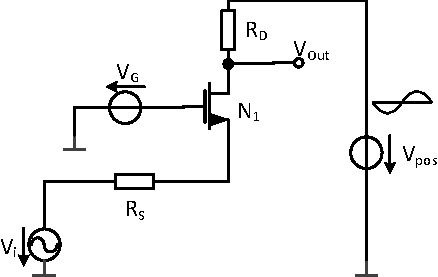
\includegraphics[width=\columnwidth, align=t]{images/03_gate_schaltung.pdf}
\end{minipage}
\hfill
\begin{minipage}[t]{0.58\columnwidth}
    \subsubsection{Verstärkung}

    \vspace{-0.2cm}

    \[
        a = \frac{v_{\rm out}}{v_{\rm in}} = \frac{R_D (1+\frac{g_o}{g_m})}{R_S + \frac{1}{g_m} + \frac{g_o}{g_m} (R_D + R_S)}
    \]

    \paragraph{Spezialfall}
    
    \vspace{-0.5cm}

    \[
        \bm{R_S = 0 \qquad  a \approx g_m \cdot r_{\rm out} \underbrace{= g_m (r_{\rm DS} \parallel R_D) }_{\text{Mikroelektronik}} }
    \]
\end{minipage}

\smallskip

Für $R_S = 0$ und $R_D \ll r_{\rm DS}$ gilt (ebenfalls in \textbf{strong inversion}) weiter: 
\[
    a \overset{R_D \text{klein}}{\approx} g_m R_D \qquad \text{bzw.} \qquad a \overset{R_D \text{gross}}{\approx} \frac{g_m}{g_o} \approx a_{\rm max}
\]

\subsubsection{Bemerkungen}
\begin{itemize}
    \item Bei den gegebenen Formeln wurde der \textbf{Body-Effekt vernachlässigt!}
    \item Ohne Body-Effekt erreicht die Gate-Schaltung die gleiche theoretisch maximal mögliche Verstärkung $a_{\rm max}$ wie die Source-Schaltung.
        Allerdings ist das Frequenzverhalten der Gate-Schaltung besser.
    \item Bei der Gate-Schaltung wird der Body-Effekt schnell zum Problem.
\end{itemize}



\subsection{Drain-Schaltung (Source-Follower)}

Die Drain-Schaltung ist eine \textbf{nichtinvertierende Verstärkerschaltung.}

\smallskip

\begin{minipage}[t]{0.4\columnwidth}
    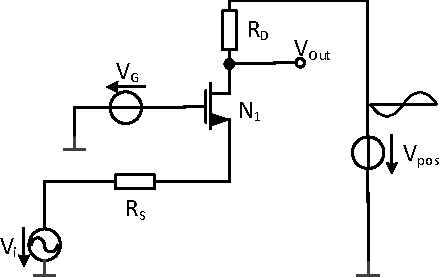
\includegraphics[width=\columnwidth, align=t]{images/03_drain_schaltung.pdf}
\end{minipage}
\hfill
\begin{minipage}[t]{0.58\columnwidth}
    \subsubsection{Verstärkung}

    \vspace{-0.2cm}
    \[
        a = \frac{v_{\rm out}}{v_{\rm in}} = \frac{R_S}{R_S + \frac{1}{g_m} + \frac{g_o}{g_m} (R_D + R_S)}
    \]

    \paragraph{Maximale Verstärkung}

    Für die \textbf{theoretisch} maximal mögliche Verstärkung $a_{\rm max}$ gilt für
    $g_m \ll g_o$ und $r_{\rm DS} \ll R_D$

    \vspace{-0.2cm}

    \[
        a_{\rm max} = \lim_{R_S \to \infty} a = \lim_{R_S \to \infty} g_m \frac{R_S}{g_m R_S + 1} = 1
    \]
\end{minipage}


\subsubsection{Level-Shift}
Die Drain-Schaltung reduziert den DC-Pegel des Ausgangssignals um die Spannung $V_{\rm GS}$. Somit ergibt sich der Zusammenhang:
\[
    V_{\rm in} - V_{\rm out} =  V_{\rm GS} = V_T + \sqrt{\frac{2 I_D}{\mu C_{\rm ox} \frac{W}{L}}} \qquad \Leftrightarrow\ \quad  V_{\rm out} = V_{\rm in} - \left( V_T + \sqrt{\frac{2 I_D}{\mu C_{\rm ox} \frac{W}{L}}} \right)
\]
Damit der Level-Shift möglichst klein ist, wird $L$ möglichst gross gewählt.


\paragraph{Body Effekt}
Da die Source nicht auf Bulk-Potential ist, muss die Veränderung der Threshold Spannung $V_T$ aufgrund des Body-Effekts berücksichtigt werden (\ref{Strong Inversion}).


\subsubsection{Bemerkungen}
\begin{itemize}
    \item Der Source-Follower hat immer eine Verstärkung $a \leq 1$
    \item Der Source-Follower bewirkt immer einen Level-Shift um $V_{\rm GS}$.
\end{itemize}



\subsection{Eingangs- und Ausgangswiderstände}

\subsubsection{Generelles Vorgehen}

\begin{itemize}
    \item Fiktive Spannungsquelle an entsprechenden Anschluss (z.B. Source) im Kleinsignalersatzschaltbild anschliessen.
    \item Strom, der über den Anschluss (z.B. Source) in den in den Transistor fliesst, messen.
    \item Widerstand als $r_i = \abs{ \frac{u_i}{i_i} }$ berechnen.
\end{itemize}


\subsubsection{Eingangs- und Ausgangswiderstände berechnen}

\paragraph{Gate $\bm{r_{i,G}}$}

\vspace{-0.2cm}

\[
    r_{i, G} \to\ \infty
\]


\paragraph{Source $\bm{r_{i,S}}$}

\vspace{-0.3cm}

\begin{align*}
    \text{Allgemein}            & \qquad r_{i, S} = \left( \frac{1}{g_m} \parallel r_{\rm DS} \right) \left( 1 + \frac{R_D}{r_{\rm DS}} \right) = \frac{1}{g_m + g_o} (1 + g_o R_D) \\
    \text{Für } r_{\rm DS} \gg R_D  & \qquad r_{i, S} \approx \frac{1}{g_m} \parallel r_{\rm DS} = \frac{1}{g_m + g_o} \\
    \text{Für } g_m \gg g_o     & \qquad r_{i, S} \approx \frac{1}{g_m}
\end{align*}


\paragraph{Drain $\bm{r_{i,D}}$}

\vspace{-0.3cm}

\begin{align*}
    \text{Allgemein}            & \qquad r_{i, D} = r_{\rm DS} \left( 1 + g_m R_S + \frac{R_S}{r_{\rm DS}} \right) = \frac{1}{g_o} (1+g_m R_S) + R_S \\
    \text{Für } r_{\rm DS} \gg R_S  & \qquad r_{i, D} \approx r_{\rm DS} \left( 1 + g_m R_S \right) = \frac{1}{g_o} (1+g_m R_S) + R_S \\
    \text{Für } R_S = 0         & \qquad r_{i, D} \approx r_{\rm DS} = \frac{1}{g_o}
\end{align*}


        \section{MOS Diode}
\subsection{Gegenüberstellung Diodentypen}

\begin{tabularx}{\columnwidth}{@{}c c c c@{}}
    Ideale Diode ($V_F = V_{F0}$) & Reale Diode & \multicolumn{2}{c}{MOS-Diode}\\
    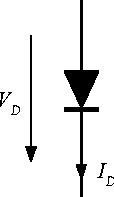
\includegraphics[height=1.75cm]{images/04_diode_ideal_symbol.pdf} & 
    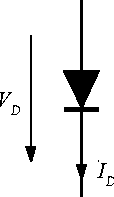
\includegraphics[height=1.75cm]{images/04_diode_real_symbol.pdf} & 
    \parbox[t]{\widthof{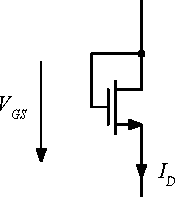
\includegraphics[height=1.75cm]{images/04_diode_nmos_symbol.pdf}}}{%
        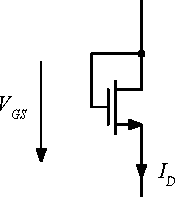
\includegraphics[height=1.75cm]{images/04_diode_nmos_symbol.pdf}\\
        \phantom{------} NMOS} & % this \phantom{------} is a bit of a hacky way to get the text to where it should be... maybe we'll change it later on
    \parbox[t]{\widthof{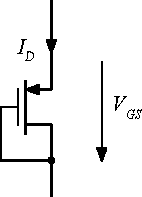
\includegraphics[height=1.75cm]{images/04_diode_pmos_symbol.pdf}}}{%
        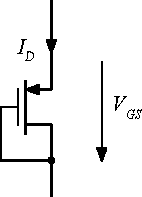
\includegraphics[height=1.75cm]{images/04_diode_pmos_symbol.pdf}\\
        PMOS} \\
    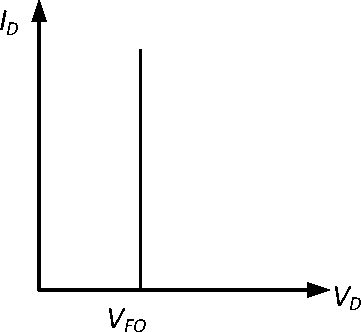
\includegraphics[width=.3\columnwidth]{images/04_diode_ideal_kennlinie.pdf} & 
    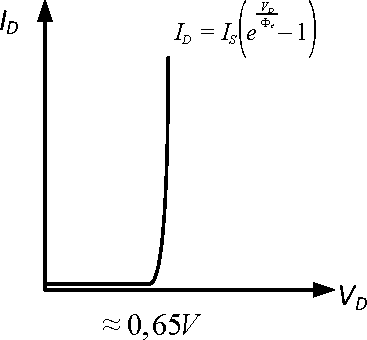
\includegraphics[width=.3\columnwidth]{images/04_diode_real_kennlinie.pdf} & 
    \multicolumn{2}{c}{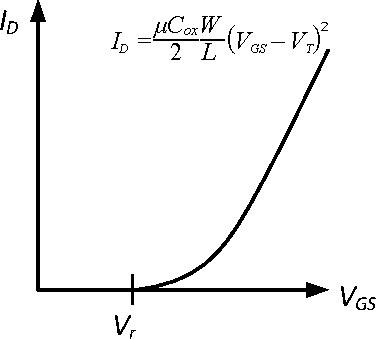
\includegraphics[width=.3\columnwidth]{images/04_diode_mos_kennlinie.pdf}} \\ 
\end{tabularx}


\subsection{Arbeitsbereich der MOS Diode}

Die MOS Diode arbeitet \textbf{(in strong inversion) immer in Sättigung}, da die Sättigungsbedingung aufgrund der Verbindung der Gate- und Source-Anschlüsse immer erfüllt ist:
\[
    V_\text{DS} = V_\text{GS} > V_\text{GS} - V_\text{T}
\]
\textbf{Hinweis:} Die Forwardspannung bestimmt, ob die MOS Diode in strong- oder weak inversion betrieben wird.
\textbf{Der 'Normalfall' ist strong inversion.}


\subsection{Arbeitspunkteinstellung}

\subsubsection{Arbeitspunkteinstellung mittels Drainstrom}

\begin{minipage}[t]{0.3\columnwidth}
    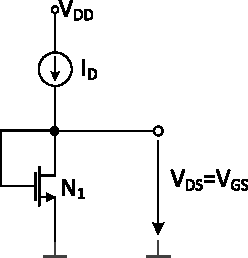
\includegraphics[width=\columnwidth, align=t]{images/04_MOS_diode_mit_stromquelle.pdf}
\end{minipage}
\hfill
\begin{minipage}[t]{0.66\columnwidth}
    Aus der Drainstrom-Gleichung (strong inversion, Sättigung) lässt sich die Spannung über der Diode als Funktion des Eingangsstroms berechnen:
    \[
        V_\text{DS} = V_\text{GS} = V_T + \sqrt{\frac{2 I_\text{D}}{\mu C_\text{ox} \frac{W}{L}}}
    \]

    \[
        V_{\rm GS} = V_\text{M} + n_{\rm M} V_\text{temp} \ln\left(\frac{I_\text{D}}{I_{\rm M}' \frac{W}{L}}\right)
    \]
\end{minipage}


\subsubsection{Arbeitspunkteinstellung mittels Seriewiderstand}

\begin{minipage}[t]{0.3\columnwidth}
    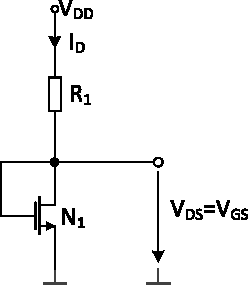
\includegraphics[width=\columnwidth, align=t]{images/04_MOS_diode_mit_widerstand.pdf}
\end{minipage}
\hfill
\begin{minipage}[t]{0.66\columnwidth}
    Der Arbeitspunkt kann auf zwei Arten ermittelt werden:

    \smallskip
    
    \begin{outline}
        \1 Grafisch durch Einzeichnen der Lastgerade des Drainwiderstands $R_1$ in der Kennlinie $I_D = f(V_{\rm GS})$
            \2 Leerlaufspannung: $V_{\rm GS,0} = V_{\rm DD}$
            \2 Kurzschluss-Strom: $I_{D, 0} = \frac{V_{\rm DD}}{R_1}$ \\
            \textrightarrow\ Schnittpunkt entspricht Arbeitspunkt
            \smallskip
        \1 Rechnerisch mittels folgender Formel
        $$ I_D = \frac{V_{\rm DD} - V_{\rm GS}}{R_1} = \frac{\mu C_{\rm ox}}{2} \frac{W}{L} (V_{\rm GS} - V_T)^2 $$
    \end{outline}
\end{minipage}


\subsection{Kleinsignalersatzschaltung}

\begin{minipage}[t]{0.3\columnwidth}
    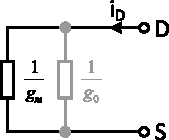
\includegraphics[width=\columnwidth, align=t]{images/04_MOS_diode_ersatzschaltung_vereinfacht.pdf}
\end{minipage}
\hfill
\begin{minipage}[t]{0.65\columnwidth}
    Die Kleinsignalersatzschaltung kann (leicht angepasst) vom MOS Transistor übernommen werden.
    \begin{align*}
        \text{Allgemein:} \quad             r_\text{\rm MD}  &= \frac{1}{g_m + g_o} = \frac{1}{g_m} \parallel r_{\rm DS} \\
        \text{\textbf{Praxis:}} \quad       r_\text{\rm MD} &\approx \frac{1}{g_m} = \frac{1}{\sqrt{2 \mu C_\text{ox} \frac{W}{L} I_\text{D}}}
    \end{align*}

\end{minipage}


\subsection{Anwendungen}

\subsubsection{Spannungsreferenz}
\label{Spannungsreferenz}

\begin{minipage}[t]{0.44\columnwidth}
    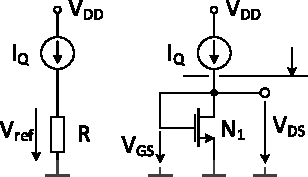
\includegraphics[width=\columnwidth, align=t]{images/04_MOS_diode_spannungsreferenz.pdf}
\end{minipage}
\hfill
\begin{minipage}[t]{0.52\columnwidth}
    \textbf{Voraussetzung: } Referenzstrom $I_Q$
    \smallskip

    \begin{itemize}
        \item[+] Kleinerer Flächenanspruch als Widerstand
        \item[+] Eingangsspannung wird durch relativ tiefen $\Delta r_{\rm MD}$ geglättet
        \item[-] Genauer als mit Widerstand, jedoch noch immer eher ungenau
        \item[-] $r_{\rm MD}$ kann nur schlecht verändert werden
    \end{itemize}
\end{minipage}


\subsubsection{Spannungsstabilisator}

\begin{minipage}[t]{0.48\columnwidth}
    \begin{outline}
        \1 MOS-Dioden Schaltung aus Abschnitt \ref{Spannungsreferenz} mit Widerstand statt Stromquelle
        \1 AC-Störung wird oberhalb von $R$ eingespeist (gegenüber GND)
    \end{outline}
\end{minipage}
\hfill
\begin{minipage}[t]{0.48\columnwidth}
    \raggedright
    
    \begin{outline}
        \1 Kleinsignalersatzschaltung des beschriebenen Aufbaus:
            \2 Spannungsteiler aus $R$ (gross) und $r_{\rm MD}$ (klein) \\
            \textrightarrow\ AC-Störspannung $v_0$ am Ausgang ($V_{\rm DS} + v_0$) sehr klein
    \end{outline}
\end{minipage}



\subsubsection{Spannungsteiler}

Spannungsteiler könnten auf mehrere Arten realisiert werden. \textrightarrow\ \textbf{Variante (b) am Besten!}

\vspace{-0.2cm}

\begin{ctabular}{@{}c cc cc cc@{}}
    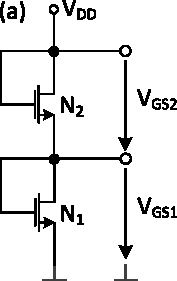
\includegraphics[height=3cm, align=t]{images/04_MOS_diode_spannungsteiler_a.pdf}    & &
    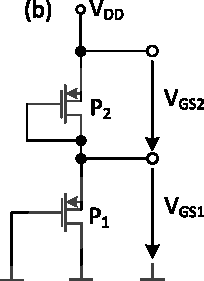
\includegraphics[height=3cm, align=t]{images/04_MOS_diode_spannungsteiler_b.pdf}    & & 
    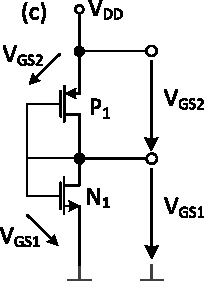
\includegraphics[height=3cm, align=t]{images/04_MOS_diode_spannungsteiler_c.pdf}    & &
    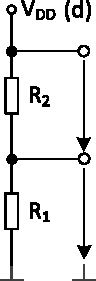
\includegraphics[height=3cm, align=t]{images/04_MOS_diode_spannungsteiler_d.pdf}    \\
\end{ctabular}


\begin{minipage}[t]{0.36\columnwidth}
    Schaltung (a)
    \begin{itemize}
        \item[+] Gleiche Elemente (nMOS)
        \item[-] Body-Effekt bei $N_2$
    \end{itemize}
   
    \smallskip

    \textbf{Schaltung (b)}
    \begin{itemize}
        \item[+] Gleiche Elemente (pMOS) \\
            \textrightarrow\ gutes Matching
        \item[+] Kein Body-Effekt
    \end{itemize}
\end{minipage}
\hfill
\begin{minipage}[t]{0.6\columnwidth}
    Schaltung (c)
    \begin{itemize}
        \item[+] Kein Body-Effekt
        \item[-] Komplementäre Elemente
            \textrightarrow\ schlechtes Matching
    \end{itemize}
   
    \smallskip

    Schaltung (d)
    \begin{itemize}
        \item[+] Gute \textbf{relative} Genauigkeit
        \item[-] Schlechte \textbf{absolute} Genauigkeit
        \item[-] Braucht viel Platz 
    \end{itemize}
\end{minipage}

\smallskip

\begin{minipage}[c]{0.55\columnwidth}
    Weil für die Ströme gilt, dass $I_{D1} = I_{D2}$ ergibt sich das das Spannungsverhältnis
\end{minipage}
\hfill
\begin{minipage}[c]{0.4\columnwidth}
    \[
        \frac{\abs{V_{\rm GS1} - V_{\rm T1}}}{\abs{V_{\rm GS2} - V_{\rm T2}}} = \sqrt{\frac{(W / L)_2}{(W / L)_1}}
    \]
\end{minipage}
        \section{MOS Stromquelle}
Bei der Einstellung des Arbeitspunkts mittels Widerstand resultiert eine quadratische Gleichung für den Strom und so die Ausgangsspannung eines Verstärkers.
Abhilfe kann eine Stromquelle anstelle des Widerstands schaffen.

MOS Transistoren sind bereits spannungsgesteuerte Stromquellen.
Durch einfügen eines $R_S$ kann der Innenwiderstand der Stromquelle \textbf{maximiert} werden. \textrightarrow\ Quelle wird 'idealer'

\subsection{Stromquelle -- Grundschaltungen}

\begin{minipage}[t]{0.44\columnwidth}
    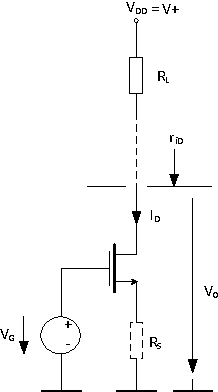
\includegraphics[width=0.48\columnwidth, align=t]{images/05_stromquelle_einfach_NMOS.pdf}
    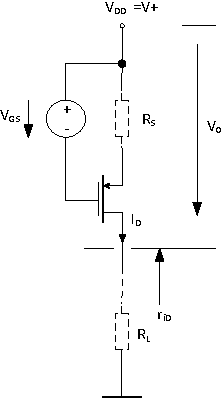
\includegraphics[width=0.48\columnwidth, align=t]{images/05_stromquelle_einfach_PMOS.pdf}
\end{minipage}
\hfill
\begin{minipage}[t]{0.5\columnwidth}
    \paragraph{Ausgangswiderstand}

    \vspace{-0.4cm}
    % \[
    %     r_{\rm iD} = r_{\rm DS} \left( 1 + g_m R_S + \frac{R_S}{r_{\rm DS}} \right) = r_{\rm DS} (1 + g_m R_S) + R_S 
    % \]

    \begin{align*}
         r_{\rm iD} &= r_{\rm DS} \left( 1 + g_m R_S + \frac{R_S}{r_{\rm DS}} \right) \\ 
                    &= r_{\rm DS} (1 + g_m R_S) + R_S
    \end{align*}
            

    \paragraph{Minimale Ausgangsspannung}

    \vspace{-0.2cm}

    \[
        V_{\rm out} = V_O > V_{O , \rm min} = R_S I_D + D_{\rm DS, sat}
    \]
\end{minipage}


\subsection{Kaskoden}
Damit für die Stromquelle kein Widerstand verwendet werden muss, kann ein weiterer Transistor verwendet werden. Diese Schaltung wird Kaskode genannt.

Dabei wird der maximale Ausgangsstrom jedoch leicht reduziert.


\subsubsection{Kaskode -- Grundschaltung}
\label{Kaskode -- Grundschaltung}

\begin{minipage}[t]{0.3\columnwidth}
    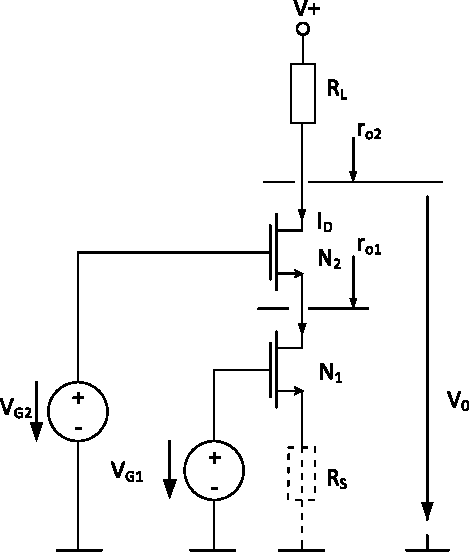
\includegraphics[width=\columnwidth, align=t]{images/05_stromquelle_kaskode.pdf}
\end{minipage}
\hfill
\begin{minipage}[t]{0.62\columnwidth}
    \paragraph{Ausgangswiderstand}

    \vspace{-0.2cm}
    \[
        r_{\rm out} = r_{\rm o2} \approx g_{m2} \cdot r_{\rm DS}^2 = a_{\rm max} \cdot r_{\rm DS}
    \]
            

    \paragraph{Minimale Ausgangsspannung}

    \vspace{-0.5cm}
    \[
        V_{O, \rm min} = V_{\rm G2} - V_{\rm GS2} + V_{\rm DS2, sat} =  V_{\rm DS1, sat} + V_{\rm DS2, sat}
    \]


    \paragraph{Strom}

    \vspace{-0.4cm}
    \[
        I_D = \frac{\mu C_{\rm ox}}{2} \left( \frac{W}{L}\right)_{N1} (V_{\rm GS\_N1} - V_T)^2 \cdot \cbl{(1 + \lambda V_{\rm DS\_N1})}
    \]
\end{minipage}


\subsubsection{Geregelte Kaskode}
Um die Kaskodenschaltung weiter zu \textbf{verbessern}, kann die $V_\text{GS}$ Spannung des oberen Transistors auf die Referenzspannung geregelt werden.
Durch das Stabilisieren der Spannung wird der Arbeitspunkt des Transistors stabilisiert (indem $I_D$ konstant ist) und der \textbf{Ausgangswiderstand noch grösser}.

\smallskip

\begin{minipage}[t]{0.55\columnwidth}
    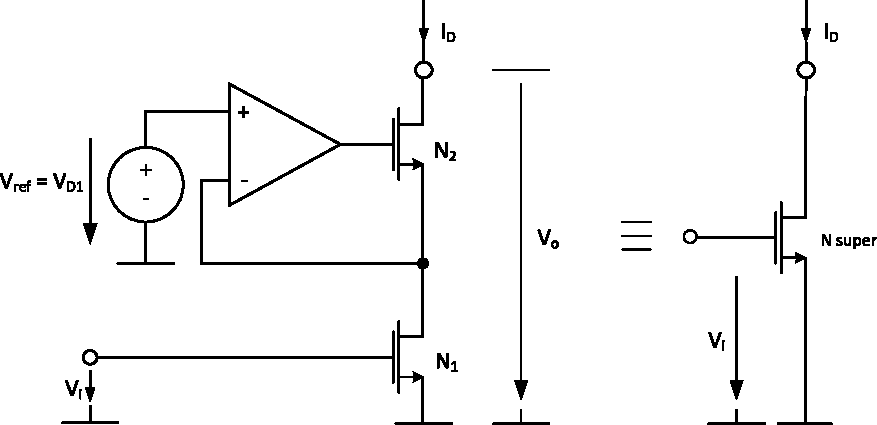
\includegraphics[width=\columnwidth, align=t]{images/05_stromquelle_geregelte_kaskode_opamp.pdf}
\end{minipage}
\hfill
\begin{minipage}[t]{0.42\columnwidth}

    \paragraph{Transkonduktanz}

    \vspace{-0.3cm}
    \[
        g_{m,\rm super} = g_{m1}
    \]            

    \paragraph{Minimale Ausgangsspannung}

    \vspace{-0.2cm}
    \[
        V_{O, \rm min} =  V_{\rm ref} + V_{\rm DS2, sat}
    \]

    \paragraph{Strom}

    \textrightarrow\ Siehe Grundschaltung (\ref{Kaskode -- Grundschaltung})
\end{minipage}


\paragraph{Ausgangswiderstand}

\vspace{-0.3cm}
\[
    r_{\rm out} \approx r_{\rm DS1} \cdot g_{m2} \cdot r_{\rm DS2} \cdot (a + 1) = \frac{1}{g_{o1}} \cdot \frac{g_{m2}}{g_{o2}} \cdot (a + 1)
\]


\subsubsection{Säckinger Kaskode}
Die Säckinger Kaskode ersetzt den komplexen OpAmp mit einem einzelnen Transistor ($\rm N_3$) in \textbf{Source-Schaltung}.

\smallskip

\begin{minipage}[t]{0.55\columnwidth}
    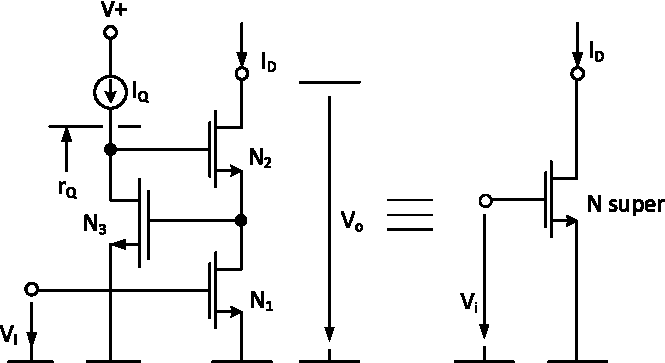
\includegraphics[width=\columnwidth, align=t]{images/05_stromquelle_geregelte_kaskode_FET.pdf}
\end{minipage}
\hfill
\begin{minipage}[t]{0.42\columnwidth}

    \paragraph{Transkonduktanz}

    \vspace{-0.3cm}
    \[
        g_{m,\rm super} = g_{m1}
    \]            

    \paragraph{Minimale Ausgangsspannung}

    \vspace{-0.2cm}
    \[
        V_{O, \rm min} =  V_{\rm GS3} + V_{\rm DS2, sat}
    \]

    \paragraph{Strom}

    \textrightarrow\ Siehe Grundschaltung (\ref{Kaskode -- Grundschaltung})
\end{minipage}


\paragraph{Ausgangswiderstand}

\vspace{-0.3cm}
\[
    r_{\rm out} \approx r_{\rm DS1} \cdot g_{m2} r_{\rm DS2} \cdot g_{m3} r_{\rm DS3} = \frac{1}{g_{o1}} \cdot \frac{g_{m2}}{g_{o2}} \cdot \frac{g_{m3}}{g_{o3}}
\]


        \section{MOS Stromspiegel}

\begin{minipage}[t]{0.48\columnwidth}
    Stromspiegel werden in \textbf{jeder} analogen integrierten Schaltung eingesetzt.
    Die möglichen Anwendungen sind:
\end{minipage}
\hfill
\begin{minipage}[t]{0.48\columnwidth}
    \begin{itemize}
        \item um Arbeitspunkte einzustellen
        \item als Eingangsstufen von OpAmps
        \item als grosse Lastwiderstände in Verstärkerschaltungen
    \end{itemize}
\end{minipage}


\subsection{Widlar Stromspiegel (Einfache Stromspiegel)}

\begin{minipage}[c]{0.35\columnwidth}
    \raggedright
    \begin{outline}
        \1 Drei Anschlüsse: \\
            SUPPLY, IN, OUT
        \1 Eingangstransistor als \textbf{Diode} beschaltet
        \1 \textbf{Ausgangstransistor muss in Sättigung bleiben}
        \1 $V_{\rm GS,1} = V_{\rm GS,2}$
    \end{outline}
\end{minipage}
\hfill
\begin{minipage}[c]{0.64\columnwidth}
    % \begin{tabular}{c c@{}}
    %     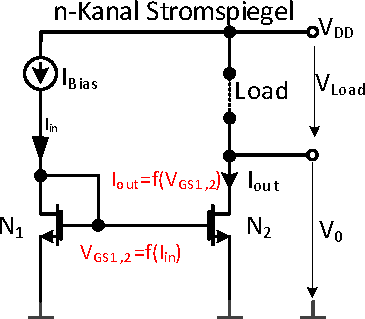
\includegraphics[height=2.3cm]{images/06_stormspiegel_nKanal.pdf} & 
    %     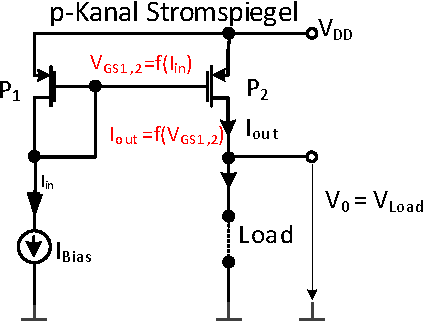
\includegraphics[height=2.3cm]{images/06_stormspiegel_pKanal.pdf}
    % \end{tabular}

     \begin{tabular}{c c@{}}
        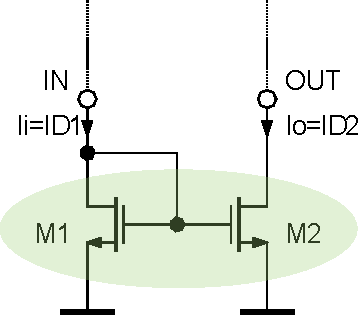
\includegraphics[height=2.2cm]{images/06_stormspiegel_widlar_nKanal.pdf} & 
        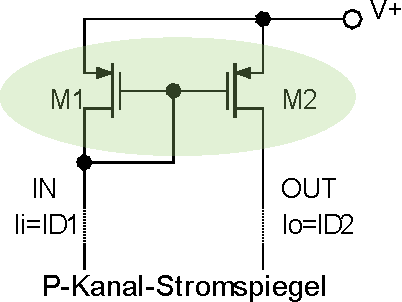
\includegraphics[height=2.2cm]{images/06_stormspiegel_widlar_pKanal.pdf}
    \end{tabular}
    
\end{minipage}


\paragraph{Wichtige Parameter}  % CHECK [Simi]: Ich weiss nicht so recht wo hin mit diesem Zeug...

\begin{minipage}[t]{0.48\columnwidth}
    \begin{outline}
        \1 Ausgangsstom $I_\text{out}$ berechnet sich aus Stromspiegelverhältnis $k$
    \end{outline}
\end{minipage}
\hfill
\begin{minipage}[t]{0.48\columnwidth}
    \begin{outline}
        \1 Eingangsimpedanz (real): $r_i = \qty{0}{\ohm}$
        \1 Ausgangsimpedanz (real): $r_o = \infty \, \qty{}{\ohm}$
    \end{outline}
\end{minipage}



\subsubsection{Arbeitspunkt festlegen}

\paragraph{Eingangsseite}

Referenzstrom aus Stromquelle oder Einstellung über Widerstand $R$

\vspace{-0.2cm}

\[
    I_\text{in} = I_\text{ref} \qquad \text{oder} \qquad I_\text{in} = \frac{V_{DD} - V_{\rm in}}{R}
\]

wobei sich die Eingangsspannung $V_{\rm in} = V_{\rm GS,1}$ aus dem Eingangsstrom berechnet als

\vspace{-0.2cm}

\[
    V_\text{in} = V_{\rm GS,1} = V_{\text{T, N}_1} + \sqrt{\frac{2 I_\text{in}}{\mu C_\text{ox}\frac{W_{\rm in}}{L_{\rm in}}}}
\]



\paragraph{Ausgangsseite}

Für Eingangs- und Ausgangstransistor soll unbedingt \textbf{das gleiche $\bm{L}$} verwendet werden.
Bei verschiedenen $L$ muss die \cbl{Kanallängenmodulation} berücksichtigt werden!

\vspace{-0.2cm}

\[
    k = \frac{I_\text{out}}{I_\text{in}} = \frac{W_\text{out}/L_\text{out}}{W_\text{in}/L_\text{in}} \cbl{ \cdot \frac{1 + \lambda_{\rm out} \cdot V_{\rm DS,out}}{1 + \lambda_{\rm in} \cdot V_{\rm DS,in}} }   \qquad \quad
    V_\text{out} \geq V_\text{DS, sat $\text{N}_2$} = \sqrt{\frac{2 I_\text{out}}{\mu C_\text{ox}\frac{W_{\rm out}}{L_{\rm out}}}}
\]

\subsubsection{Kleinsignalersatzschaltung / Kleinsignalparameter}

\begin{minipage}[t]{0.48\columnwidth}
    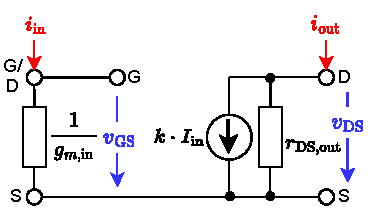
\includegraphics[width=\columnwidth, align=t]{images/06_stromspiegel_kleinsignalersatzschaltung.pdf}
\end{minipage}
\hfill
\begin{minipage}[t]{0.48\columnwidth}

    \begin{align*}
        r_{\rm in}  &\approx \frac{1}{g_{\rm m, in}} = \frac{1}{\sqrt{2 \mu C_{ox} \frac{W_{\rm in}}{L_{\rm in}} I_{\rm in}}} \\
        r_{\rm out} &= \frac{1}{g_{o1}} \approx \frac{V_{E2}}{I_{\rm out}} = \frac{a_E \cdot L}{I_{\rm out}}
    \end{align*}
    

\end{minipage}


\subsubsection{Optimierungen für kleinstmögliche Toleranzen}

\begin{tabular}{cl}
    $V_{\rm T1} = V_{\rm T2}$               & \textrightarrow\ Beide Transistoren brauchen dieselbe konstante Temperatur    \\
    $\mu C_\text{ox1} = \mu C_\text{ox2}$   & \textrightarrow\ Matching durch gute Platzierung (Common Centroid Layout)     \\
    $\lambda_1 = \lambda_2$                 & \textrightarrow\ Identische Länge $L$ (und möglichst gross) 
\end{tabular}

\smallskip

Grundsätzlich können Stromspiegel auch in Weak- und Moderate-Inversion betrieben werden.
Dabei leidet jedoch die Genauigkeit.


\subsection{Anwendungen von Stromspiegeln}

\begin{outline}
    \1 Senken-Quellen-Inversion
    \1 Verbesserung Power Supply Rejection; DC-Level Shifting \\
        \textrightarrow\ Umlenkung von $R_L$ nach GND statt Laststrom von $V_{\rm DD}$ zu Last   % NOTE: [Simi] Bild würde ich aktuell weglassen
    \1 Stromquellenlast bei Differenzstufe (siehe Abschnitt XXX) %TODO [Simi]: Referenz auf OpAmp Abschnitt, sobald existent
    \1 Erzielen eines hohen Lastwiderstands
\end{outline}


% Da $V_\text{T}$ Temperaturabhängig ist, sollten die Transistoren jeweils dieselbe Temperatur haben.

% Ebenfalls ist das Teilverhältnis von $\mu C_\text{ox}$ abhängig.
% Durch kontrolliertes Platzieren der Transistoren (Common Centroid Layout) und gute Temperaturkontrolle beim Herstellen können diese Werte relativ genau gehalten werden.

% Zu guter Letzt sollten die $\lambda$ gleich gross sein.
% Dazu müssen die Transistoren dieselbe Länge $L$ (und in einem nächsten Schritt möglichst gross) sein.


\subsection{Mehrfachstromspiegel}

%NOTE: [Simi] Wenn mehr Platz benötigt wird, Bild weglassen und nur Text verwenden

\begin{minipage}[t]{0.48\columnwidth}
    Mit einem Referenzstrom werden mehrere Ausgangsströme generiert. 
    Die Grösse der vom Stromspiegel erzeugten Ströme kann durch die Länge und Breite der Transistoren eingestellt werden.
\end{minipage}
\hfill
\begin{minipage}[t]{0.48\columnwidth}
    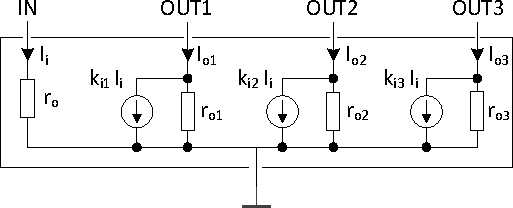
\includegraphics[width=\columnwidth, align=t]{images/06_mehrfachstromspiegel.pdf}
\end{minipage}



\subsection{Wilson-Stromspiegel (3-Transistor-Schaltung)}
Im Vergleich zum Widlar-Stromspiegel besitzt der Wilson-Stromspiegel eine \textbf{grössere Ausgangsimpedanz}.
$\text{N}_3$ bildet dabei eine Rückkopplung zur Regelung von $I_\text{o}$ auf $I_\text{i}$.
% TODO: [Flurin] How does this work? idgi...

\begin{minipage}[c]{0.35\columnwidth}
    \raggedright
    \begin{outline}
        \1 Eingangstransistor als Stromquelle beschaltet
        \1 Ausgangstransistor als \textbf{Diode} beschaltet
        \1 \textbf{T3 muss in Sättigung bleiben}
        \1 Bei gleicher Geometrie: $V_{\rm GS,2} = V_{\rm GS,3}$
    \end{outline}
\end{minipage}
\hfill
\begin{minipage}[c]{0.64\columnwidth}
     \begin{tabular}{c c@{}}
        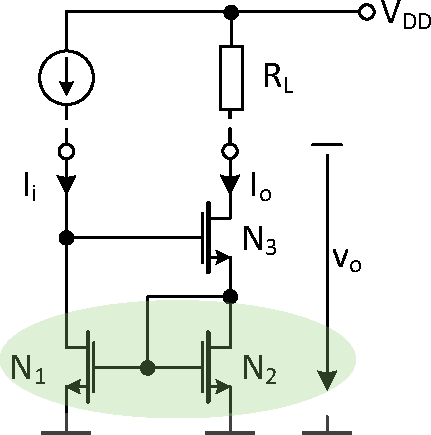
\includegraphics[height=2.9cm, align=t]{images/06_stormspiegel_wilson_nKanal.pdf} & 
        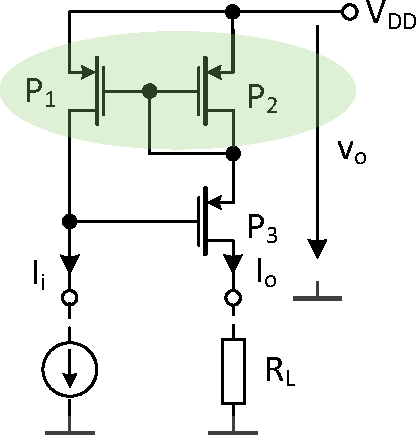
\includegraphics[height=2.9cm, align=t]{images/06_stormspiegel_wilson_pKanal.pdf}
    \end{tabular}
    
\end{minipage}


\subsubsection{Kenngrössen}
\label{Kenngrössen Wilson}

\vspace{-0.4cm}

\begin{align*}
    V_0         &\geq V_{\rm GS,2} + V_{\rm DS,sat3} = 2 V_{\rm GS} - V_T = V_T + 2 \sqrt{ \frac{2 I_O}{\mu C_{\rm OX} \frac{W_{\rm out}}{L_{\rm out}}} }                                                                                           \\
    V_I         &= 2 V_{\rm GS} = 2 V_T + 2 \sqrt{ \frac{2 I_I}{\mu C_{\rm OX} \frac{W_{\rm in}}{L_{\rm in}}} }                                                                                                                                     \\
    r_{\rm out} &\approx \frac{1}{g_{o3}} \left( 1 + \frac{g_{m3}}{g_{m2}} + \frac{1}{g_{o1}} \cdot \frac{g_{m3} g_{m1}}{g_{m2}} \right) \underset{\rm N1 = N2}{=} \frac{1}{g_o} \left( 2 + \frac{g_m}{g_o} \right) = r_{\rm DS} \cdot (2 + g_m \cdot r_{\rm DS})
\end{align*}



\subsection{Verbesserter Wilson-Stromspiegel / Kaskoden-Stromspiegel}

\begin{minipage}[t]{0.35\columnwidth}
    \begin{center}
        \textbf{\myul{Verbesserter Wilson}}

        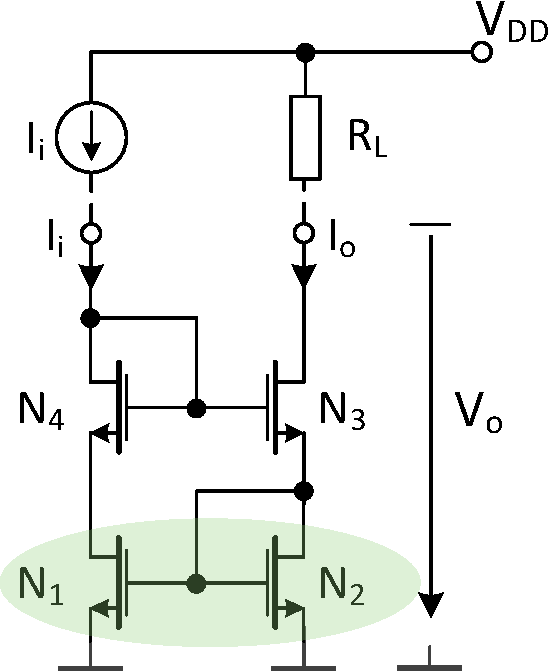
\includegraphics[width=\columnwidth, align=t]{images/06_stormspiegel_wilson_verbessert.pdf}
    \end{center}
\end{minipage}
\hfill
\begin{minipage}[t]{0.35\columnwidth}
    \begin{center}
        \textbf{\myul{Kaskode}}

        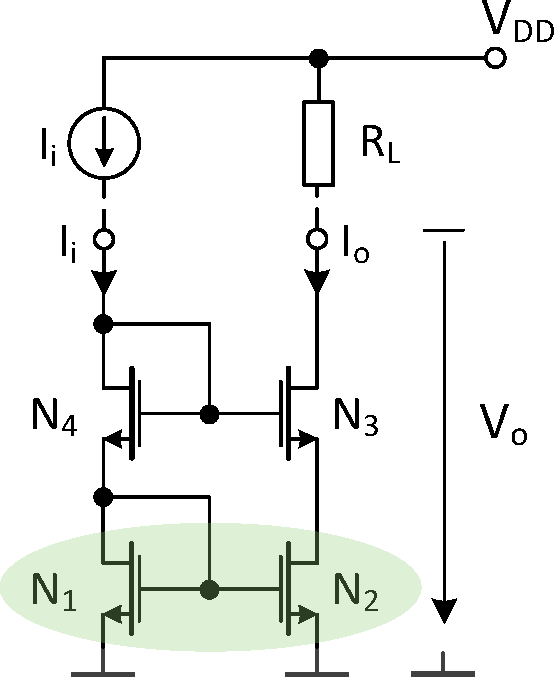
\includegraphics[width=\columnwidth, align=t]{images/06_stormspiegel_kaskode.pdf}
    \end{center}
\end{minipage}


\subsubsection{Kenngrössen}

Die Kenngrössen für beide Stromspiegel berechnen sich gleich wie diejenigen des Wilson-Stromspigels.
\textrightarrow\ Siehe Abschnitt \ref{Kenngrössen Wilson}

\columnbreak


\subsection{Stromspiegel mit geregelter Kaskode}

Durch M4 und M5 wird die Spannung am Gate von M2 konstant gehalten. % CHECK[Simi] @Flurin: Stimmt das? Auf V7 S24 steht V_{DS2} wird konstant gehalten
So wird die Ausgangsimpedanz bedeutend erhöht.


\begin{minipage}[t]{0.42\columnwidth}
    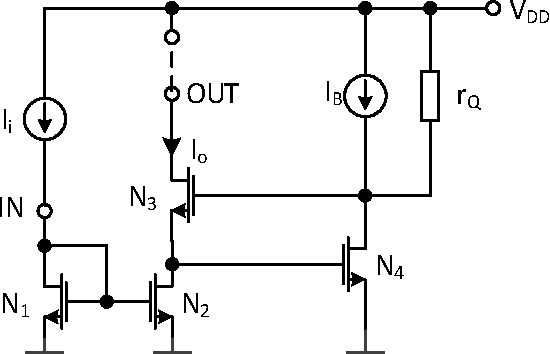
\includegraphics[width=\columnwidth, align=t]{images/06_stormspiegel_geregelte_kaskode.pdf}

\end{minipage}
\hfill
\begin{minipage}[t]{0.56\columnwidth}
    % \subsubsection{Kenngrössen}

    \vspace{-0.4cm}

    \begin{align*}
        V_0         &\geq V_{\rm GS,4} + V_{\rm DS,sat3} = V_T + (1..2) \sqrt{ \frac{2 I_O}{\mu C_{\rm OX} \frac{W_{\rm out}}{L_{\rm out}}} }                                                                                           \\
        V_I         &= V_{\rm GS,1} = 2 V_{T,1} + \sqrt{ \frac{2 I_{\rm in}}{\mu C_{\rm OX} \frac{W_{\rm in}}{L_{\rm in}}} }                                                                                                                                     \\
        r_{\rm out} &\approx \frac{1}{g_o} \left( \frac{g_m}{g_o} \right)^2 = r_{\rm DS} \cdot (g_m r_{\rm DS})^2
    \end{align*}
\end{minipage}


\subsection{Gegenüberstellung der Stromspiegel}

%NOTE [Simi] Sooo viel bringt diese Tabelle auch nicht... Die ganze Info steht bei der jeweiligen Schaltung aber bei genug Platz kann man sie schon drin lassen -> Inhalt ist aber eher klein...
\resizebox{\columnwidth}{!}{
    \renewcommand{\arraystretch}{2}
    \begin{tabular}{|c|c|c|c|c|}
    \hline
    \textbf{Typ}    & \textbf{Genauigkeit}  & $\bm{r_{\rm out}}$                                            & $\bm{V_{\rm I}}$                                                              & $\bm{V_{\rm O,min}}$                                                              \\
    \hline
    Widlar          & +                     & $\frac{1}{g_o}$                                               & $\approx V_T + \sqrt{ \frac{2I_I}{\mu C_{\text{ox}} \frac{W_I}{L_I}} }$       & $\approx \sqrt{ \frac{2I_O}{\mu C_{\text{ox}} \frac{W_O}{L_O}} }$                 \\
    \hline
    Wilson          & +                     & $\approx \frac{1}{g_o} \left( 2 + \frac{g_m}{g_o} \right)$    & $\approx 2V_T + 2 \sqrt{ \frac{2I_I}{\mu C_{\text{ox}} \frac{W_I}{L_I}} }$    & $\approx V_T + 2 \sqrt{ \frac{2I_O}{\mu C_{\text{ox}} \frac{W_O}{L_O}} }$         \\
    \hline
    Verb. Wilson    & ++                    & $\approx \frac{1}{g_o} \left( 2 + \frac{g_m}{g_o} \right)$    & $\approx 2V_T + 2 \sqrt{ \frac{2I_I}{\mu C_{\text{ox}} \frac{W_I}{L_I}} }$    & $\approx V_T + 2 \sqrt{ \frac{2I_O}{\mu C_{\text{ox}} \frac{W_O}{L_O}} }$         \\
    \hline
    Kaskode         & ++                    & $\approx \frac{1}{g_o} \left( 2 + \frac{g_m}{g_o} \right)$    & $\approx 2V_T + 2 \sqrt{ \frac{2I_I}{\mu C_{\text{ox}} \frac{W_I}{L_I}} }$    & $\approx V_T + 2 \sqrt{ \frac{2I_O}{\mu C_{\text{ox}} \frac{W_O}{L_O}} }$         \\
    \hline
    Ger. Kaskode    & ++                    & $\approx \frac{1}{g_o} \left( \frac{g_m}{g_o} \right)^2$      & $\approx V_T + \sqrt{ \frac{2I_I}{\mu C_{\text{ox}} \frac{W_I}{L_I}} }$       & $\approx V_T + (1..2) \sqrt{ \frac{2I_O}{\mu C_{\text{ox}} \frac{W_O}{L_O}} }$    \\
    \hline
    \end{tabular}
    \renewcommand{\arraystretch}{1}
}

%TODO: [Flurin] Plots der verschidenen Varianten V7S24
% Evtl. bessere Darstellungen? Warscheindlich nicht lohnenswert.
% NOTE: [Simi] Würde ich komplett wegglassen


        \input{sections/07_MOS_verstärker.tex}
        \section{Frequenzverhalten}

Da jede leitende Fläche eine Kapazität gegenüber der umliegenden Flächen besitzt, müssen zur Einschätzung des Frequenzgangs diverse Kapazitäten berücksichtigt werden.

\subsection{Parasitäre Kapazitäten in MOS-Transistoren}
%TODO: Evtl. Bild wie in V9S8
%TODO: Kleinsignalersatzschaltung eines Transistors inkl. Kapazitäten

\subsubsection{Nutzkapazität}
\[
    C_{oxt} = C_{ox} \cdot W_{eff} \cdot L_{eff}
\]

\subsubsection{Parasitäre Kapazitäten}
Gate-Drain- und Gate-Source-Kapazitäten durch Overlap
\[
    C_{GDt} = C_{GD} \cdot W_{eff} \cdot L_{eff}
    \qquad
    C_{GSt} = C_{GS} \cdot W_{eff} \cdot L_{eff}
\]

Source-Bulk- und Drain-Bulk-Kapazitäten durch Raumladungszone
\[
    C_{jSBt} = C_{jSB} \cdot A_S + C_{jswSB} \cdot P_S
    \qquad
    C_{jDSt} = C_{jGS} \cdot A_S + C_{jswDB} \cdot P_D
\]
$C_{jsw}$: Side Wall Kapazität
$P$: Perimiter

Kanal-Bulk-Kapazität durch Raumladungszone
\[
    C_{jBCt} = C_{jBC} \cdot W_{eff} \cdot L_{eff}
\]

Junction-Bulk-Kapazität
\[
    C_{jBC}
\]

\subsection{Vereinfachtes Handrechenmodell}

% TODO: Ersatzschaltung und Formeln aus V9S11

\begin{tabular}{lllll}
    Arbeitsbereich & & & & \\
    Gesättigt & & & & \\
    Ungesättigt & & & & \\
\end{tabular}

\subsection{Miller-Effekt}
% TODO: Bild der equivalenten Schaltungen
Das Miller Theorem postuliert, dass die linke Schaltung durch Wählen von $Y_1$ und $Y_2$ als 
\[
    Y_1(s) = Y(s) (1+A) \quad\text{und}\quad Y_2(s) = Y(s) (1+\frac{1}{A})
\]
äquivalent gemacht werden können.
Es kann durch einfaches Einsetzen bewiesen werden.

Die Miller-Kapazität $C_m$ erscheint 
\begin{itemize}
    \item multipliziert mit $1+\abs{A}$ am Eingang als $C_{mi}$ und
    \item multipliziert mit $1+\abs{\frac{1}{A}}$ am Ausgang als $C_{mo}$.
\end{itemize}

Nachteile: 
\begin{itemize}
    \item Durch Verschieben des Miller-C aus dem Vorwärtspfad stimmt die UTF nach Ersetzen des $C_m$ nicht mehr.
    \item Das Miller-Theorem geht von konstantem Frequenzgang der Verstärkung aus. Es stimmt folglich nur für die tieferen Frequenzen.
\end{itemize}

\subsubsection{Approximatives Frequenzverhalten}
Schlecht.
%TODO: Evtl. Berechnung aus V9S15-17 -> Nein, nur beschreiben, warum diese für nichts zu brauchen ist.

\subsection{Frequenzverhalten durch Zero Value Time Constant Analysis}


\subsubsection{Vorgehen}
\begin{enumerate}
    \item Kleinsignalersatzschaltung erstellen.
    \item Für alle $C_k$ die zugehörige Zeitkonstante bestimmen.
    \begin{enumerate}
        \item Alle übrigen $C_{i \neq k} = 0$ setzen.
        \item Durch Ersetzen des $C_k$ mit einer Stromquelle den von $C_k$ her gesehenen Kleinsignalwiderstand bestimmen.
        \item Zeitkonstante als $\tau_k = R_k C_k$ bzw. Polfrequenz als $f_{pk} = \frac{1}{2 \pi \tau_k}$ berechnen.
    \end{enumerate}
    \item Approximierter Frequenzgang aus DC-Verstärkung und den Polstellen zusammensetzen.
\end{enumerate}

\subsubsection{Resultate}
Das GBP ist gegeben durch den ersten Pol: 
$GPB \approx f_{p1} \cdot A_{DC}$

Die Stabilität wird bestimmt durch den zweiten Pol:
$f_{180^\circ} \approx f_{p2}$

\subsubsection{Typische Werte}
%TODO: Tabelle aus V9S23
%TODO: Typische Widerstandswerte analog V9S22
Vorsicht bei $C_{GD}$: Sollte der Transistor eine Spannungsverstärkung haben, so muss der Miller-Effekt berücksichtigt werden.

Weiter ist $C_{GD}$ bei hohen Frequenzen oft als erstes kurzgeschlossen, für den zweiten Pol muss dieser als kurzgeschlossen betrachtet werden.



        \input{sections/09_MOS_operationsverstärker.tex}
        \section{Stabilität / Frequenzverhalten von OpAmps}

\subsection{UTF des rückgekoppelten Verstärkers}

\begin{minipage}[c]{0.53\columnwidth}
    \includegraphics[width=\columnwidth, align=t]{images/10_stabilitaet_loop.pdf}
\end{minipage}
\hfill
\begin{minipage}[c]{0.46\columnwidth}
    \vspace{-0.2cm}
    \begin{align*}
         A_{\rm CL}(s)  &= \frac{U_{\rm out}(s)}{U_{\rm in}(s)} = \frac{A(s)}{1+ \underbrace{ A(s) F(s) }_{T(s)}} \\
                        &= \frac{1}{\frac{1}{A(s)} + F(s)} \overset{\text{tiefe Freq.}}{\approx} \frac{1}{F(s)}
    \end{align*}
\end{minipage}

\begin{ctabular}{ll | ll}
    $A(s)$  & Frequenzgang des Verstärkers      & $T(s)$    & Loop Gain     \\
    $F(s)$  & Frequenzgang der Rückkopplung     &           &               \\
\end{ctabular}


\subsection{Stabilitätskriterien}
Der \textbf{Nenner} von $A_{\rm CL}(s)$ darf \textbf{nicht null} sein, da das System sonst schwingt. \\
Um die Stabilität zu beurteilen werden Verstärkungs- und Phasenmarge betrachtet.

\smallskip
Damit ein System stabil ist, müssen die beiden folgenden Bedingungen für Verstärkungsmarge und Phasenmarge erfüllt sein:


\begin{minipage}[t]{0.48\columnwidth}
    \paragraph{Verstärkungsmarge}

    Bei $\Phi = \qty{-180}{\degree}$ ablesen:

    \[
        \text{GM} = g_M = \abs{A(s) \cdot T(s)} \overset{!}{<} 1
    \]

    \smallskip

    \paragraph{Phasenmarge}

    Bei Verstärkung $1$ bzw  $\qty{0}{\decibel}$ ablesen:
    \[
        \text{PM} = \varphi_M = \qty{180}{\degree} + \Phi \overset{!}{>} \qty{0}{\degree}
    \]
\end{minipage}
\hfill
\begin{minipage}[t]{0.48\columnwidth}
    \includegraphics[width=\columnwidth, align=t]{images/10_bode_plot_V2.pdf}
\end{minipage}

% Für Stabilität muss die Verstärkungsmarge 
% \[
%     GM = g_M = \left.\abs{T(s)} \right|_{\angle T(S) = 180^\circ} < 1
% \]
% sein.

% Die Phasenmarge muss
% \[
%     PM = \phi_M = 180^\circ - \Phi =  \left. 180^\circ - \angle T(s) \right|_{\abs{T(s)} > 0^\circ}
% \]
% erfüllen.


\subsubsection{Überschwingen der Sprungantwort}

Die Phasenmarge bestimmt, wieviel die Sprungantwort überschwingt.

\vspace{-0.2cm}

\begin{ctabular}{ll}
    \textbf{Phasenmarge}                & \textbf{Verhalten der Sprungantwort}              \\
    $\phi_M \leq \qty{0}{\degree}$      & Gegengekoppelter Verstärker schwingt selbständig  \\
    $\phi_M > \qty{0}{\degree}$         & Stabil, mit gedämpftem Überschwingen              \\
    $\phi_M = \qty{65}{\degree}$        & Einziger Überschwinger mit $\qty{4.7}{\percent}$  \\
    $\phi_M \geq \qty{75}{\degree}$     & Einbussen bei der Slew-Rate                       \\
\end{ctabular}

\vspace{-0.2cm}



\subsection{OpAmp als System mit 2 Polen}

\begin{minipage}[c]{0.54\columnwidth}
    \begin{outline}
        \1 1. Pol (bei $f_{\rm d}$) bestimmt Bandbreite (GBW)
        \1 2. Pol (bei $f_{\rm nd}$) bestimmt die Stabilität \\
            \textrightarrow\ Phasenmarge $\varphi_M$
    \end{outline}
\end{minipage}
\hfill
\begin{minipage}[c]{0.42\columnwidth}
    \[
        \varphi_M = \qty{90}{\degree} - \arctan \left( \frac{\text{GBW}}{f_{\rm nd}} \right)
    \]
\end{minipage}


\subsubsection{Design-Regeln für Stabilität des OpAmps}

\begin{outline}
    \1 1. Pol muss in erster Stufe (Differenzstufe) realisiert werden
    \1 2. Pol bei ca. $3 \cdot \text{GBW}$ wählen \textrightarrow\ $\varphi_M \approx \qty{72}{\degree}$ (fast kein Überschwingen)
\end{outline}


        \section{Realisierungsformen von OpAmps}

\subsection{Einstufiger OTA}

\subsubsection{Differenzstufe mit (Stromspiegel) Last}

%NOTE: [Simi] @Flurin Ich würde hier aus Platzgründen nicht noch einmal das Schema der Differenzstufe einfügen... Wir wissen langsam, wie das Ding aussieht...
Die Differenzstufe des OpAmps realisiert einen einstufigen OTA.
Meist werden aber 'verbesserte' Realisierungsformen verwendet. 

\vspace{-0.3cm}

\[
    a = - g_{\rm m, N1, N2} \cdot \underbrace{ \left( r_{\rm N,P} \parallel r_{\rm DS} \right) }_{r_{\rm out}} \qquad 
    \text{BW} \approx f_d = \frac{1}{2\pi r_{\rm out} C_{\rm L}} \qquad 
    \text{GBW} = f_d \cdot \abs{a} = \frac{g_{\rm m, N1, N2}}{2\pi C_{\rm L}}
\]

\begin{itemize}
    \item[-] Meist ungenügende Verstärkung, da die Last zu klein ist.
    \item[-] Eingangs- und Ausgangs-Common-Mode-Bereich nicht unabhängig wählbar.
\end{itemize}


\subsubsection{Telescopic Cascode OTA}
\label{Telescopic Cascode OTA}

\begin{minipage}[t]{0.35\columnwidth}
    \includegraphics[width=\columnwidth, align=t]{images/11_OTA_einstufig_kaskode.pdf}
\end{minipage}
\hfill
\begin{minipage}[t]{0.62\columnwidth}
    %CHECK: [Simi] @ Flurin: stimmt das so mit den Vorzeichen bei der Verstärkung a ? g_m negativ, r positiv -> a negativ (invertierend)
    \[
        a = g_{\rm m, N1, N2} \cdot \underbrace{ \left( r_{\rm K\_N} \parallel r_{\rm K\_P} \right) }_{r_{\rm out}} 
    \]
    \[
        r_{\rm K\_N, K\_P} \approx r_{\rm DS} \cdot (2+ g_m \cdot r_{\rm DS})
    \]
    \[
        \text{BW} \approx f_d = \frac{1}{2\pi r_{\rm out} C_{L}} \qquad \text{GBW} = f_d \cdot \abs{a} = \frac{g_{\rm m, N1, N2}}{2 \pi C_{L}}
    \]

    \smallskip

    \begin{itemize}
        \item[-] Eingangs- und Ausgangs-Common-Mode-Bereich nicht unabhängig wählbar
        \item[-] Kleinerer Ausgangsspannungsbereich
        \item[+] Geringer Stromverbrauch
        \item[+] Hohe Verstärkung
    \end{itemize}
\end{minipage}


\subsubsection{Folded Cascode OTA}

\begin{minipage}[t]{0.5\columnwidth}
    \includegraphics[width=\columnwidth, align=t]{images/11_OTA_einstufig_gefaltete_kaskode.pdf}
\end{minipage}
\hfill
\begin{minipage}[t]{0.48\columnwidth}
    Die Berechnungsformel für die den Folded Cascode OTS sind gleich wie beim Telescopic Cascode OTA. 
    \textrightarrow\ Abschnitt \ref{Telescopic Cascode OTA}

    \smallskip

    \begin{itemize}
        \item[+] Hohe Verstärkung
        \item[+] Eingangs- und Ausgangs-Common- \\
            Mode-Bereich unabhängig wählbar
        \item[-] Hoher Stromverbrauch (meist doppelt im Vergleich zu Telescopic)
    \end{itemize}
\end{minipage}



\subsubsection{Symmetrischer OTA}
\begin{minipage}[t]{0.48\columnwidth}
    \includegraphics[width=\columnwidth, align=t]{images/11_OTA_einstufig_symmetrisch.pdf}
\end{minipage}
\hfill
\begin{minipage}[t]{0.48\columnwidth}
    %CHECK [Simi] @Flurin: stimmt das so mit den Vorzeichen bei der Verstärkung a? g_m negativ, r positiv -> a negativ (invertierend)
    \[
        a_V = B \cdot  g_{\rm m\_N1} \cdot \left( r_{\rm DS\_N3} \parallel r_{\rm DS\_P3} \right)
    \]
    \[
        f_d = f_{\rm P\_Nout} = \frac{1}{2 \pi \cdot R_{\rm Nout} \cdot C_{\rm Nout}}
    \]
    \[
        f_d \approx \frac{1}{2 \pi \left( r_{\rm DS\_N3} \parallel r_{\rm DS\_P3} \right) C_L}
    \]
    \[
        \text{GBW} = \abs{a_V} \cdot f_d = B \cdot \frac{g_{\rm m\_N1}}{2 \pi C_{\rm Nout}} \approx B \cdot \frac{g_{\rm m\_N1}}{2 \pi C_L}
    \]
\end{minipage}

\smallskip

\begin{itemize}
    \item[+] Besseres Verhalten bei hohen Frequenzkompensation, einstellbar durch $B$
    \item[+] Grosser Aussteuerbereich
    \item[+] Sehr hohe Frequenz des zweiten Pols \textrightarrow\ stabil
\end{itemize}


\subsection{Zweistufige OTA}

\subsubsection{Zweistufiger OTA}

\begin{minipage}[t]{0.5\columnwidth}
    \includegraphics[width=\columnwidth, align=t]{images/11_OTA_zweistufig.pdf}
\end{minipage}
\hfill
\begin{minipage}[t]{0.48\columnwidth}
    \[
        a_V = \cgn{a_{\rm V1}} \cdot \cvt{a_{\rm V2}} 
    \]
    \[
        \cgn{a_{\rm V1}} = g_{\rm m, N1, N2} (r_{\rm DS\_N2} \parallel r_{\rm DS\_P2})
    \]
    \[
        \cvt{a_{\rm V2}} = g_{\rm m, P3} (\rm r_{DS\_N3} \parallel r_{\rm DS\_P3} \parallel R_L)
    \]
    \[
        f_{\rm p,N1} = \frac{1}{2\pi r_{\rm N1} C_{\rm N2}} \qquad f_{\rm p,N3} = \frac{1}{2\pi r_{L} C_{L}}
    \]
\end{minipage}

\smallskip

\begin{minipage}[t]{0.35\columnwidth}
    \begin{itemize}
        \item[+] Grosse Verstärkung
    \end{itemize}
\end{minipage}
\hfill
\begin{minipage}[t]{0.63\columnwidth}
    \begin{itemize}
        \item[-] $C_2 \gg C_L$ nötig für Stabilität \textrightarrow\ suboptiomal
        \item[-] Durch $C_C$ tiefere Bandbreite
    \end{itemize}
\end{minipage}



\subsubsection{Miller-OTA}

Durch 'Verlagerung' der Kapazität $C_C$ wirkt diese als Miller-Kapazität. 
Somit werden die \textbf{Pole auseinandergeschoben} ohne viel Chipfläche für eine grosse Kapazität zu benötigen.
Die \textbf{Bandbreite} des Miller-OTA ist folglich \textbf{kleiner}, jedoch hat die Eigenschaft der Stabilität das grössere Gewicht.

\smallskip

\begin{minipage}[t]{0.48\columnwidth}
    \includegraphics[width=\columnwidth, align=t]{images/11_OTA_zweistufig_miller.pdf}
\end{minipage}
\hfill
\begin{minipage}[t]{0.48\columnwidth}
    \begin{outline}
        \1 \cbl{N2} ist dominierendenr Knoten \textrightarrow\ $f_{\rm pN2}$
        \1 Bei hohe Frequenzen wirkt $C_C$ als Kurzschluss zw. Gate und Drain von $P_3$ \textrightarrow\ Diodenschaltung \textrightarrow\ $f_{\rm pN3}$
        \1 $C_C$ erzeugt eine Nullstelle, deren Lage mit einem $R_C$ in Serie 'platziert' werden kann
    \end{outline} 
\end{minipage}


\renewcommand{\arraystretch}{1.8}
\begin{ctabular}{ll}
    Dominanter Pol                  & $f_{\rm pN2} = \frac{1}{2 \pi R_{\rm n2} \left( C_{\rm n2} + A_{\rm V2} C_C \right)} \approx \frac{1}{2 \pi R_{\rm n2} A_{\rm V2} C_C}$                           \\
    $\qty{3}{\decibel}$-Bandbreite  & $\text{BW} \approx f_d = f_{\rm N2} = \frac{1}{2 \pi R_{\rm N2} A_2 C_C}$                                                                                         \\
    Verstärkung $a$                 & $a = a_1 \cdot a_2 = g_{\rm m\_N1,2} \, R_{\rm N2} \cdot g_{\rm m\_P3} \, R_{\rm N3}$                                                                             \\
    Gain-Bandwidth-Product          & $\text{GBW} = a \cdot f_d = \frac{g_{\rm m\_N1,2} \, R_{\rm N2} \cdot g_{\rm m\_P3} \, R_{\rm N3}}{2 \pi R_{\rm N2} a_2 C_C} = \frac{g_{\rm m\_N1,2}}{2 \pi C_C}$ \\ 
    Nicht-Dominanter Pol            & $f_{\rm nd} = f_{\rm N3} = \frac{1}{2 \pi R_{\rm n3} C_L} \approx \frac{g_{\rm m\_P3}}{2 \pi C_L}$                                                                \\ 
    Phasenmarge $\varphi_M$         & $\varphi_M = \qty{90}{\degree} - \arctan \left( \frac{\text{GBW}}{f_{\rm nd}} \right)$                                                                            \\
\end{ctabular}
\renewcommand{\arraystretch}{1}


% \subsubsection{Design-Regeln}
% \begin{itemize}
%     \item $\left. \abs{A(s)F(s)} \right|_{\phi = 180^\circ} < 1$
%     \item $\left. \angle (A(s)F(s)) \right|_{\abs{A(s)F(s)} = 1} > 180^\circ$
%     \item Zweiter Pol bei ca. $3 \cdot GBW$ wählen
% \end{itemize}


        \section{OTA Designbeispiel}

\subsection{Spezifikationen}

Für die vorgegebenen Spezifikationen soll eine Schaltung entwickelt werden.

\vspace{-0.3cm}

\begingroup
\setlength{\columnseprule}{0pt}
\begin{multicols}{2}
    \begin{description}
        \item[Open Loop Gain] $a_\text{OL}$
        \item[Last] $C_\text{L}$
        \item[GBW]  
        \item[Phase Margin] $\Phi_\text{M}$
        \item[Stabilität] Unity gain stable or not
        \item[Slew Rate] SR
        \item[Versorgungsspannung] $V_\text{CC}$
        \item[Output Swing]
        \item[Offset Voltage] $V_\text{OS}$
    \end{description}
\end{multicols}
\endgroup



\subsection{Designablauf}

\begin{minipage}[t]{0.6\columnwidth}
    \includegraphics[width=\columnwidth, align=t]{images/12_OTA_design.pdf}
\end{minipage}
\hfill
\begin{minipage}[t]{0.38\columnwidth}   % NOTE: [Simi] @Flurin: So ganz zufrieden bin ich damit nicht... vielleicht sollten wir doch besser das Enum nehmen...
    \raggedright

    \paragraph{Front-End-Design}
    Der OTA ist typischerweise ein Sub-Block einer grösseren Schaltung.
    Es wird ein erster Schaltungsentwurf erstellt.
    Bei der Simulation können (mangels Layout) noch keine parasitären Effekte berücksichtigt werden.

    \medskip

    \paragraph{Back-End Design}
    Das Layout des OTAs wird gezeichnet. 
    Extraktion fügt der Netzliste parasitäre Komponenten zu, was eine sehr wirklichkeitsnache Simulation des Designs erlaubt.

    \medskip

    \paragraph{Production}
    Ev. wird OTA (allenfalls mit weiteren kritischen Komponenten) auf einem Prototyp integriert und evaluiert.
    Häufig wird auch die gesamte Schaltung als Prototyp realisiert. 

    \medskip

    \textbf{Hinweis:} Nur das Front-End Design ist Gegenstand dieser Vorlesung!
\end{minipage}



% \begin{enumerate}
%     \item Spezigikation: Definition der Ein- und Ausgänge einer Schaltung\label{enum:spec}
%     \item Handrechnungen, Erstellen eines Schaltplanes
%     \item Schaltkreissimulation
%     \item Spezifikationen erfüllt? Ja: gut. Nein: zurück zu Schritt~\ref{enum:spec}
%     \item Layout\label{enum:layout}
%     \item Schaltkreissimulation mit parasitären Einflüssen
%     \item Spezifikationen erfüllt? Ja: gut. Nein: zurück zu Schritt~\ref{enum:layout}
%     \item Herstellen eines Prototypen\label{enum:prototyp}
%     \item Test und Evaluation
%     \item Spezifikationen erfüllt? Ja: gut. Nein: zurück zu Schritt~\ref{enum:prototyp}
%     \item Produktion
% \end{enumerate}

% Wenn an irgendeinem Punkt festgestellt wird, dass die Spezifikationen nicht erreicht werden können, muss zurük zu Schritt~\ref{enum:spec} zurück gesprungen werden.

\columnbreak



\subsection{Front End Design}

Für das Fornt-End Design wird grundsätzich immer das gleiche Vorgehen angewendet, unabhängig von der Umsetzung des OTAs.

\smallskip

\begin{enumerate}
    \item Gegeben (Specs / Schaltungstopologie) und Gesucht (meist $I_{\rm bias}$, $\frac{W}{L}$ der Transistoren) niederschreiben
    \item Grossignalanalyse: APs von von jedem Knoten (von Ausgang zu Eingang) bestimmen \textrightarrow\ Jeweils $V$ und $I$
    \item Kleinsignalparameter bestimmen: $g_\text{m}$, $r_\text{DS}$
    \item Kleinsignalanalyse durchführen: GBW und DC-Verstärkung bestimmen
    \item Stabilität uns Aussteuergrenzen kontrollieren
    \item Simulation zur Kontrolle
\end{enumerate}


\subsubsection{Grossignalanalyse}

\begin{itemize}
    \item Sicherstellen, dass alle Transistoren \textbf{gesättigt} sind \textrightarrow\ meist nur in \textbf{strong inversion}
    \item Slew Rate bestimmt Biasstrom der Ausgangsstufe: $I_\text{bias} = \text{SR} \cdot C_\text{L}$
    \item Min. $\frac{W}{L}$ der Ausgangsstufe wird durch Aussteuergrenze bestimmt: $V_\text{DS, sat} = \sqrt{\frac{2 I_\text{D}}{\mu C_\text{ox} \frac{W}{L}}}$
    \item Bei mehrstufigen Verstärkern: Non-Dominanter Pol bei $f_\text{nd} = 3 \cdot \text{GBW}$ wählen \\
        \textrightarrow\ Bestimmt $L$ der 2. Stufe
    \item Bei mehrstufigen Verstärkern: Biasstrom der ersten Stufe mit $\frac{W}{L}$ bestimmen.
\end{itemize}


\subsubsection{Kleinsignalparameter}

In Sättigung (strong inversion) wird der Arbeitspunkt durch den Strom $I_{\text{bias}} = I_{\rm D}$ bestimmt

\vspace{-0.1cm}

\[
    g_{\rm m} = \sqrt{2 I_\text{D} \cdot \mu C_\text{ox} \cdot \frac{W}{L}} \qquad \qquad
    r_{\rm DS} = \frac{a_{\rm E} \cdot L + V_\text{DS}}{I_\text{D}}
\]


\subsubsection{Kleinsignalanalyse}

\begin{itemize}
    \item GBW und DC-Verstärkung gemäss verwendeter Schaltungstopologie bestimmen
\end{itemize}

\smallskip

\paragraph{Auswirkungen einzelner Parameter bei zweistufigen OTAs}
Eine Vergrösserung des Parameters links führt zu den rechtsgezeugten Reaktionen.

\smallskip

\renewcommand{\arraystretch}{1.3}
\resizebox{\columnwidth}{!}{
    \begin{tabular}{|l || c|c|c|c|}
        \hline
        \textbf{Vergrösserung von...}                                           & $\bm{A_0}$                    & \textbf{GBW}              & \textbf{SR}       & $\bm{C_L}$    \\
        \hline\hline
        Strom in Eingangsstufe $I_{\rm B}$                                      & $\downarrow^{\frac{1}{2}}$    & $\uparrow^{\frac{1}{2}}$  & $\uparrow$        &               \\
        \hline
        Strom in Ausgangsstufe                                                  & $\downarrow^{\frac{1}{2}}$    &                           &                   &               \\
        \hline
        $\frac{W}{L}$ der Eingangstransistoren (N$_1$, N$_2$)                   & $\uparrow^{\frac{1}{2}}$      & $\uparrow^{\frac{1}{2}}$  &                   &               \\
        \hline
        $\frac{W}{L}$ des Ausgangstransistors (P$_3$)                           & $\uparrow^{\frac{1}{2}}$      &                           &                   &               \\
        \hline
        $L$ der nicht-Stromspiegel Transistoren (N$_1$, N$_2$, P$_1$ - P$_3$)   & $\uparrow$                    &                           &                   &               \\
        \hline
        $\frac{W}{L}$ des Ausgangstransistors (P$_3$)                           & $\uparrow^{\frac{1}{2}}$      & $\uparrow^{\frac{1}{2}}$  &                   &               \\
        \hline
        Kompensationskapazität                                                  &                               & $\downarrow$              & $\downarrow$      & $\uparrow$    \\
        \hline
    \end{tabular}
}
\renewcommand{\arraystretch}{1}



% \begin{enumerate}
%     \item Gegeben und Gesucht niederschreiben
%     \item Grossignalanalyse: APs von Ausgang zu Eingang bestimmen.
%     \begin{enumerate}[a]
%         \item Sicherstellen, dass alle Transistoren gesättigt sind.
%         \item Oft kommt nur Strong Inversion in Frage.
%         \item Slew Rate bestimmt Biasstrom d. Ausgangsstufe: $I_\text{bias} = SR \cdot V_\text{L}$
%         \item Aussteuergrenze bestimmt min. $\frac{W}{L}$ d. Ausgangsstufe: $V_\text{DS, sat} = \sqrt{2 I_\text{D} / (\mu C_\text{ox} W/L)}$
%         \item Bei mehrstufigen Verstärkern: Non-Dominanter Pol bei $f_\text{nd} = 3 \cdot GBW$ wählen \textrightarrow Bestimmt $L$ der 2. Stufe.
%         \item Bei mehrstufigen Verstärkern: Biasstrom der ersten Stufe mit $\frac{W}{L}$ bestimmen.
%     \end{enumerate}
%     \item Kleinsigalanalyse: $g_\text{m}$, $r_\text{DS}$, GBW und DC-Verstärkung bestimmen.
%     \begin{enumerate}[a]
%         \item $g_m = \sqrt{2I_\text{D} \cdot \mu C_\text{ox} \cdot W/L}$
%         \item $r_{ds} = (a_\text{a} L + V_\text{DS}) / I_\text{D}$
%         \item $GBW = a \cdot f_\text{d}$ bestimmt $g_\text{m}$ bestimmt $W/L$ des Transistors mit dominantem Pol $f_\text{d} = 1/(2\pi \cdot r_\text{out} \cdot C_\text{L})$
%         \item DC-Verstärkung d.\ letzten Stufe bestimmen.
%         \item $SR_1$ der ersten Stufe als $SR_1 = SR/a_2$ berechnen.
%     \end{enumerate}
%     \item Stabilität uns Aussteuergrenzen kontrollieren
%     \item Simulation zur Kontrolle
% \end{enumerate}

% \paragraph{Spezielles zum Miller OTA:}

% % TODO: [Flurin] Sorry, I missed some of this... Would probably need to be more detailed? if included at all
% % NOTE:[Simi] @Flurin Ich habe mal nur auf die entsprechende Schaltung verwiesen... Ich denke, das genügt schon...
% \[
%     f_p \approx g_m / (2\pi C_L)
% \]
% \[
%     GBW \approx g_m / (2\pi R a C_C)
% \]


\subsection{Designgleichungen}
%TODO: Designgleichungen Miller OTA V14S3

        \section{Infrastruktur eines Chips}
% TODO: Übersicht aus V14S12

\subsection{Spannungsversorgung}
Ein wichtiger Teil der Infrastruktur ist die Spannungsversorgung. 
Die benötigte Leistung kann wie folgt abgeschätzt werden.
\[
    P_\mathrm{dynamisch} = f(C, f, N, U^2)
\]
\[
    P_\mathrm{statisch} = I_\mathrm{leakage} \cdot U^2
\]

\subsection{Arbeitspunkteinstellung}
Zur Arbeitspunkteinstellung gibt es verschiedene Strategien.
Diese können für einen der unten aufgeführten Punkte ausgelegt werden.
\begin{itemize}
    \item Konstante Spannungsamplitude
    \item Konstante Ströme
    \item Konstante Verstärkung un Transkonduktanz
\end{itemize}

\subsubsection{Verteilungsarten}
\paragraph{Voltage Mode:}

Vorteil:
\begin{itemize}
    \item Minimale Hardware
\end{itemize}
Nachteil:
\begin{itemize}
    \item Schlechtes Matching (aufgrund von Technologie und Temperaturvariationen)
    \item Störungen auf der Verbindungsleitung
\end{itemize}

\paragraph{Current Mode:}

Vorteile:
\begin{itemize}
    \item Gutes Matching (Stromspiegeltransistoren am gleichen Ort)
    \item Weniger störanfällig wegen niederohmigen Signalen
\end{itemize}
Nachteil:
\begin{itemize}
    \item Mehr Hardware
    \item Höherer Stromverbrauch
\end{itemize}

\subsection{Referenzschaltungen}
Spannungsregler sowie Arbeitspunkteinstellung und verschiedene Blöcke benötigen eine absolute Referenz.

Relative Genauigkeiten bis ca. 0.1\% ist ohne trimmen möglich, während absolute Referenzwerte Losabweichungen von bis zu 40\% aufweisen.

Entsprechend müssen absolute Referenzen trimmbar realisiert werden können.

Als Richtwert für die Qualität einer Referenz wird die Sensitivität $S$ des Referenzwerts auf die Änderung einer externen Grösse.

\subsubsection{Spannungsteiler}
$S = 1$ auf Versorgungsspannungsänderungen \textrightarrow\ unbrauchbar.

\subsubsection{Bootstrap-Referenz}
% TODO: Schema V14S16
\[
    I_D = I_M' \frac{W}{L} e^{\frac{V_{GS}-V_M}{n m V_\mathrm{temp}}}
\]
\[
    V_{GS} - V_M = n_m V_\mathrm{temp} \ln{\frac{I_D}{I_M' \frac{W}{L}}}
\]
\[
    \Delta V_{GS} = n_m V_\mathrm{temp} \ln\left(\frac{I_{D1}}{I_{D2}} \frac{(W/L)_2}{(W/L)_1}\right)
\]
\[
    I_\mathrm{bias} = \frac{\Delta V_{GS}}{R_2}
\]
$R_2$: Externer Präzisionswiderstand

Vorteile:
\begin{itemize}
    \item Unabhängig von Versorgungsspannung
\end{itemize}
Nachteile:
\begin{itemize}
    \item Proportional zur Temperatur
\end{itemize}

\textrightarrow\ Benötigt eine Start-Up Schaltung, da $I_D = \qty{0}{\ampere}$ auch stabil wäre. (nicht gezeichnet)

\subsubsection{Bandgap-Referenz}
\paragraph{Grundprinzip}
% TODO: Bild aus V14S17

Temperaturkoeffizient einer Diode: 
\[
    TC_D = \qty{-2}{\milli\volt\per\kelvin} = \frac{d V_D}{dT} \approx \frac{V_D-V_{BG}}{T}
\]

Temperaturkoeffiziend von $V_\mathrm{temp}$:
\[
    TD_{V\mathrm{temp}} = \frac{d V_\mathrm{temp}}{d T} = \frac{k}{e} \approx \qty{86.24\cdot10^{-6}}{\volt\per\kelvin} 
\]

Faktor $k$:
\[
    k = -\frac{TC_D}{TC_{V\mathrm{temp}}} = \frac{\qty{-2}{\milli\volt\per\kelvin}}{\qty{86.24\cdot10^{-6}}{\volt\per\kelvin}} = 23.2
\]

\paragraph{Realisierung}
%TODO: Schema aus V14S18

Die Bandgap-Referenz wird durch Bipolartransistoren realisert.
Die Emitter-Basis-Diode liefert dabei die Diodenspannung.
\[
    V_D = V_{EB} = V_\mathrm{temp} \ln \frac{-I_C}{I_S' A_E}
\]
%TODO: Entweder alle Formeln aus V14S18/19 oder zumindest beschreiben, wie k eingestellt wird.

Vorteile:
\begin{itemize}
    \item Unabhängig von Versorgungsspannung
    \item \qty{10}{ppm\per\kelvin} bei (\qty{0}{\degreeCelsius}-\qty{70}{\degreeCelsius})
\end{itemize}
Nachteile:
\begin{itemize}
    \item Die Spannung $V_\mathrm{ref}$ sowie der Temperaturkoeffizient hängt stark vom Offset des OpAMPs ab. \textrightarrow\ Trimmen
    \item Es ist eine Startup-Schaltung nötig.
\end{itemize}

        \part{Basics}
        \section{Grundwissen}

\subsection{Bodediagramm zeichnen}
\resizebox{\columnwidth}{!}{
    \begin{tabular}{|c|c|c|}
        \hline
        \multirow{2}{*}{Element} & \multicolumn{2}{c|}{Frequenzgang} \\
        \cline{2-3}
        & Amplitudengang & Phasengang \\
        \hline
        Polstelle & $-\qty{20}{\decibel\per Dekade}$, $-\qty{3}{\decibel}$ bei der Polstelle & $-90^\circ$, $-45^\circ$ bei der Polstelle \\
        \hline
        Nullstelle & $+\qty{20}{\decibel\per Dekade}$, $+\qty{3}{\decibel}$ bei der Nullstelle & $+90^\circ$, $+45^\circ$ bei der Nullstelle \\
        \hline
    \end{tabular}
}

\medskip%

Der Anstieg / Abfall der Phase beginnt jeweils eine Dekade vor der Pol- bzw Nullstelle.

\subsection{Dezibel}
Werte in Dezibel sind immer \textbf{Leistungsverhältnisse}. 
Wird mit Spannungen gerechnet, so muss die Spannung quadriert oder der Wert in Dezibel verdoppelt werden.

\[
    g_{\qty{}{\decibel}} = 10 \cdot \log_{10} \left( \frac{P_{\rm out}}{P_{\rm in}} \right) = 20 \cdot \log_{10} \left( \frac{U_{\rm out}}{U_{\rm in}} \right)
\]

%TODO: [Flurin] Kennlinie aus V10S9
%CHECK: [Simi] @Flurin: WHY??????


    \end{layout}
\end{document}
